\documentclass[UTF8,11pt]{ctexart}
\usepackage[margin=1in]{geometry}
\usepackage{amsmath,amssymb,booktabs,array,longtable,graphicx,xurl}
\usepackage[hidelinks]{hyperref}
\usepackage{tikz,placeins,needspace}
\usetikzlibrary{arrows.meta}
\setlength{\emergencystretch}{3em}
\newcommand{\R}{\mathbb{R}}
\newcommand{\ES}{\operatorname{ES}}
\newcommand{\supp}[1]{\href{supplement.pdf\##1}{科学补充材料}}
\newcommand{\audit}[1]{\href{audit-notes.pdf\##1}{审查记录}}
% Generated from original public aggregate values; no inference.
\newcommand{\FullES}{477.85}
\newcommand{\InertialES}{824.73}
\newcommand{\FullFDE}{1326.09}
\newcommand{\FullADE}{636.11}
\newcommand{\InertialDelta}{-346.87}
\newcommand{\PointRowFull}{Full & 73.77 & 332.31 & 812.26 & 1326.09\\}
\newcommand{\PointRowGMM}{GMM & 71.92 & 323.79 & 792.99 & 1299.11\\}
\newcommand{\PointRowdtThreeHundred}{dt300 & 75.88 & 340.10 & 825.76 & 1335.73\\}
\newcommand{\PointRowInertial}{Inertial & 31.17 & 237.93 & 934.03 & 2095.78\\}

\author{}
\date{公开审阅修订稿，2026年10月9日；署名待确认}

\title{科学补充材料：拟合预测器、完整比较与复现规格}
\begin{document}\maketitle\hypertarget{sec:models}{}
本文是独立科学阅读文档，不再把执行日志接在论文本体后。
新增图示使用不变公开汇总，后接详细规格与完整表。
历史保存评分题注对应其捕获版本；当前有限算法状态为14实际等价、七证据不足，
分辨率不变状态全为证据不足。重组不修复保留失败或科学缺口。
版本、执行与审查回应另见\href{audit-notes.pdf}{审查记录}。

\section{地形几何与十配置设计}
\begin{figure}[htbp]\centering
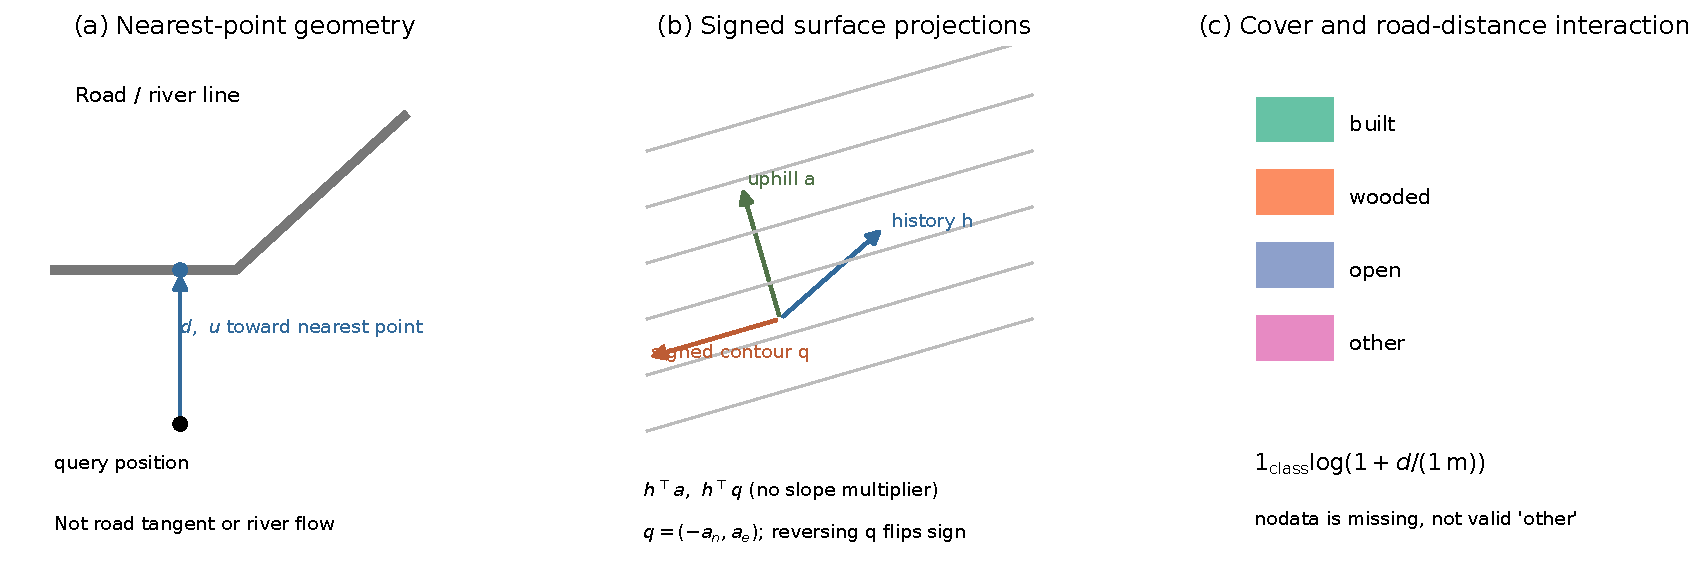
\includegraphics[width=\linewidth]{../figures/revision46-v1/revision46-geometry.pdf}
\caption{几何示意而非真实路线。左：道路／河流最近点、距离及指向该点的方向，不是切线或流向。
中：带符号历史$h$、上坡$a$、等高线$q$的不同点积与坡度大小。
右：覆盖类别和保留道路距离的组合；无效查询不是有效“其他”覆盖类。
正文列明排除的道路类别。图内英文标签与本题注逐项对应。}
\label{fig:terrain-geometry}\hypertarget{fig:terrain-geometry}{}\end{figure}
\begin{figure}[htbp]\centering
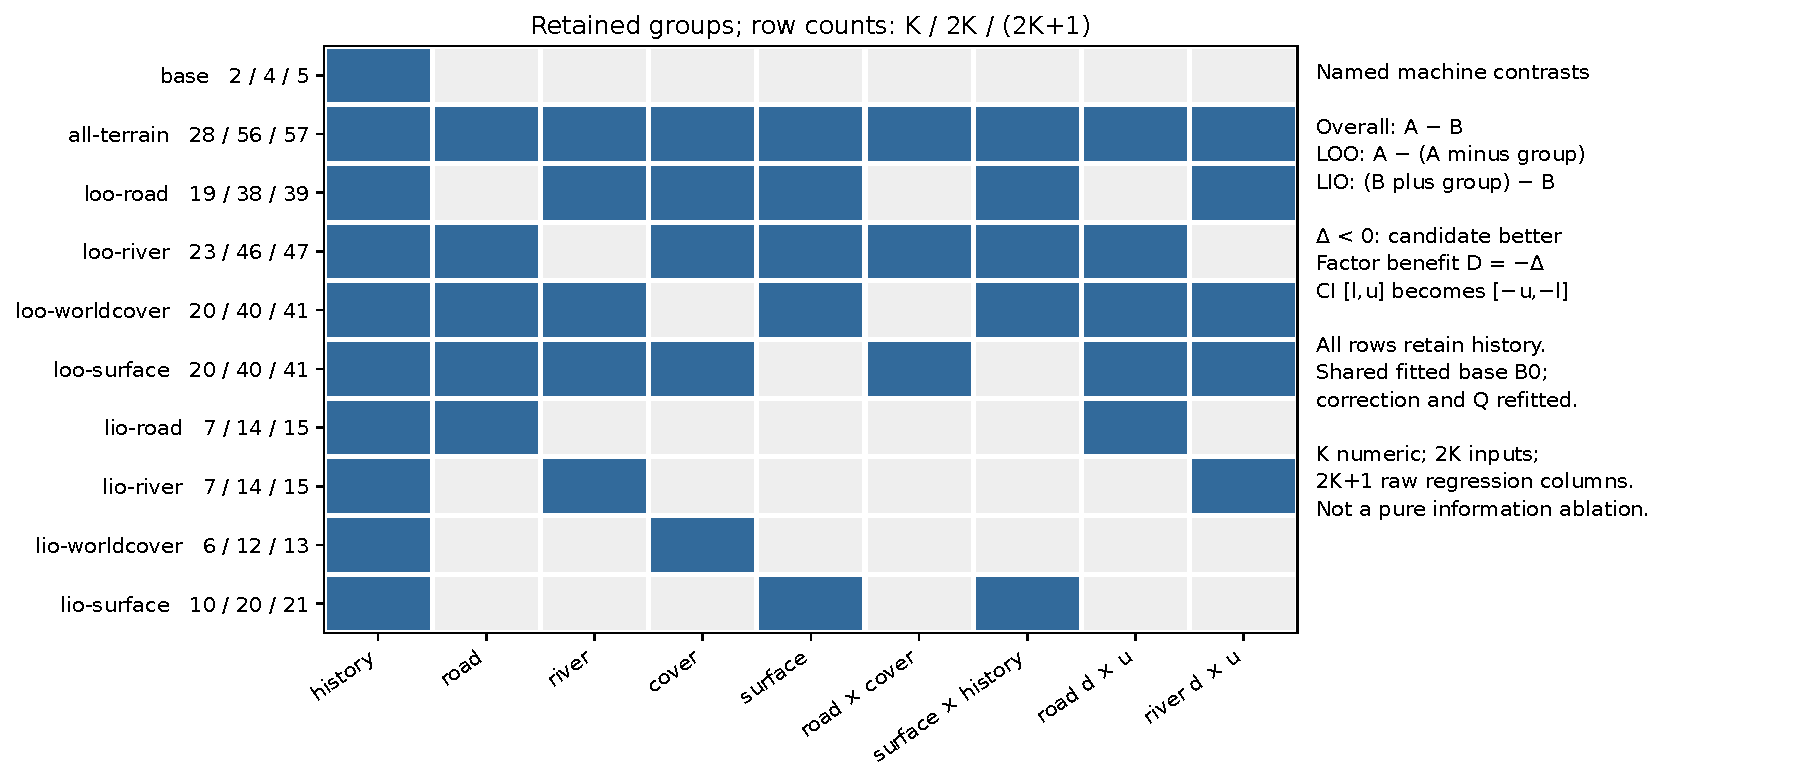
\includegraphics[width=\linewidth]{../figures/revision46-v1/revision46-design-matrix.pdf}
\caption{十个独立拟合配置。道路--覆盖交互依赖两个父组，坡面--历史在LIO-surface仍保留。
$K$为数值特征数，不是全部设计列数。LOO机器候选为all-terrain、对照为all-minus-group；
若写成移除损失的因素收益，需要反转符号和区间端点。
LIO比较history-plus-group与base。图示不改变家族或非加性交互定义。}
\label{fig:terrain-matrix}\end{figure}\FloatBarrier

\section{互补误差与不确定性视图}
\begin{figure}[htbp]\centering
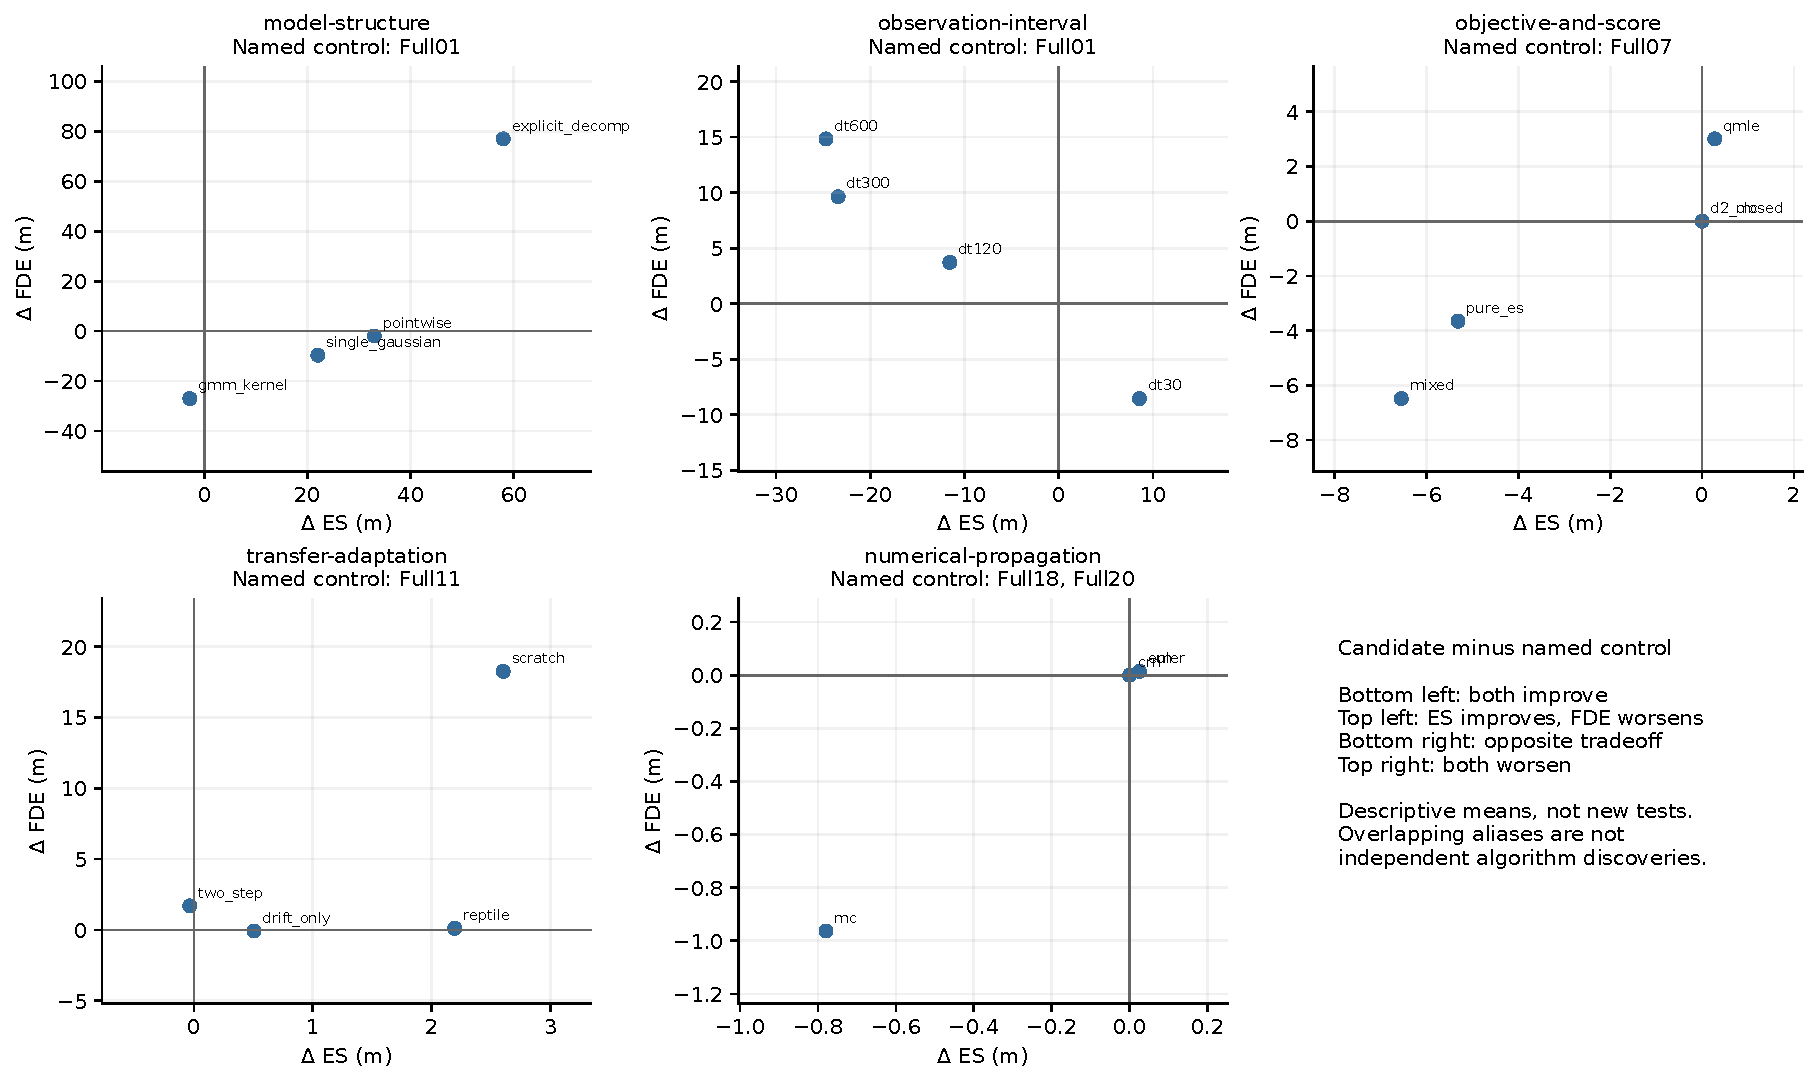
\includegraphics[width=\linewidth]{../figures/revision46-v1/revision46-score-error-tradeoff.pdf}
\caption{全部21项候选减具名对照：加权ES与均值位置FDE（米），两轴均负差有利。
分面保留原家族，各Full对照不合并。这是配对均值描述，不是新联合检验或Pareto排名。}
\label{fig:tradeoff}\end{figure}
\begin{figure}[htbp]\centering
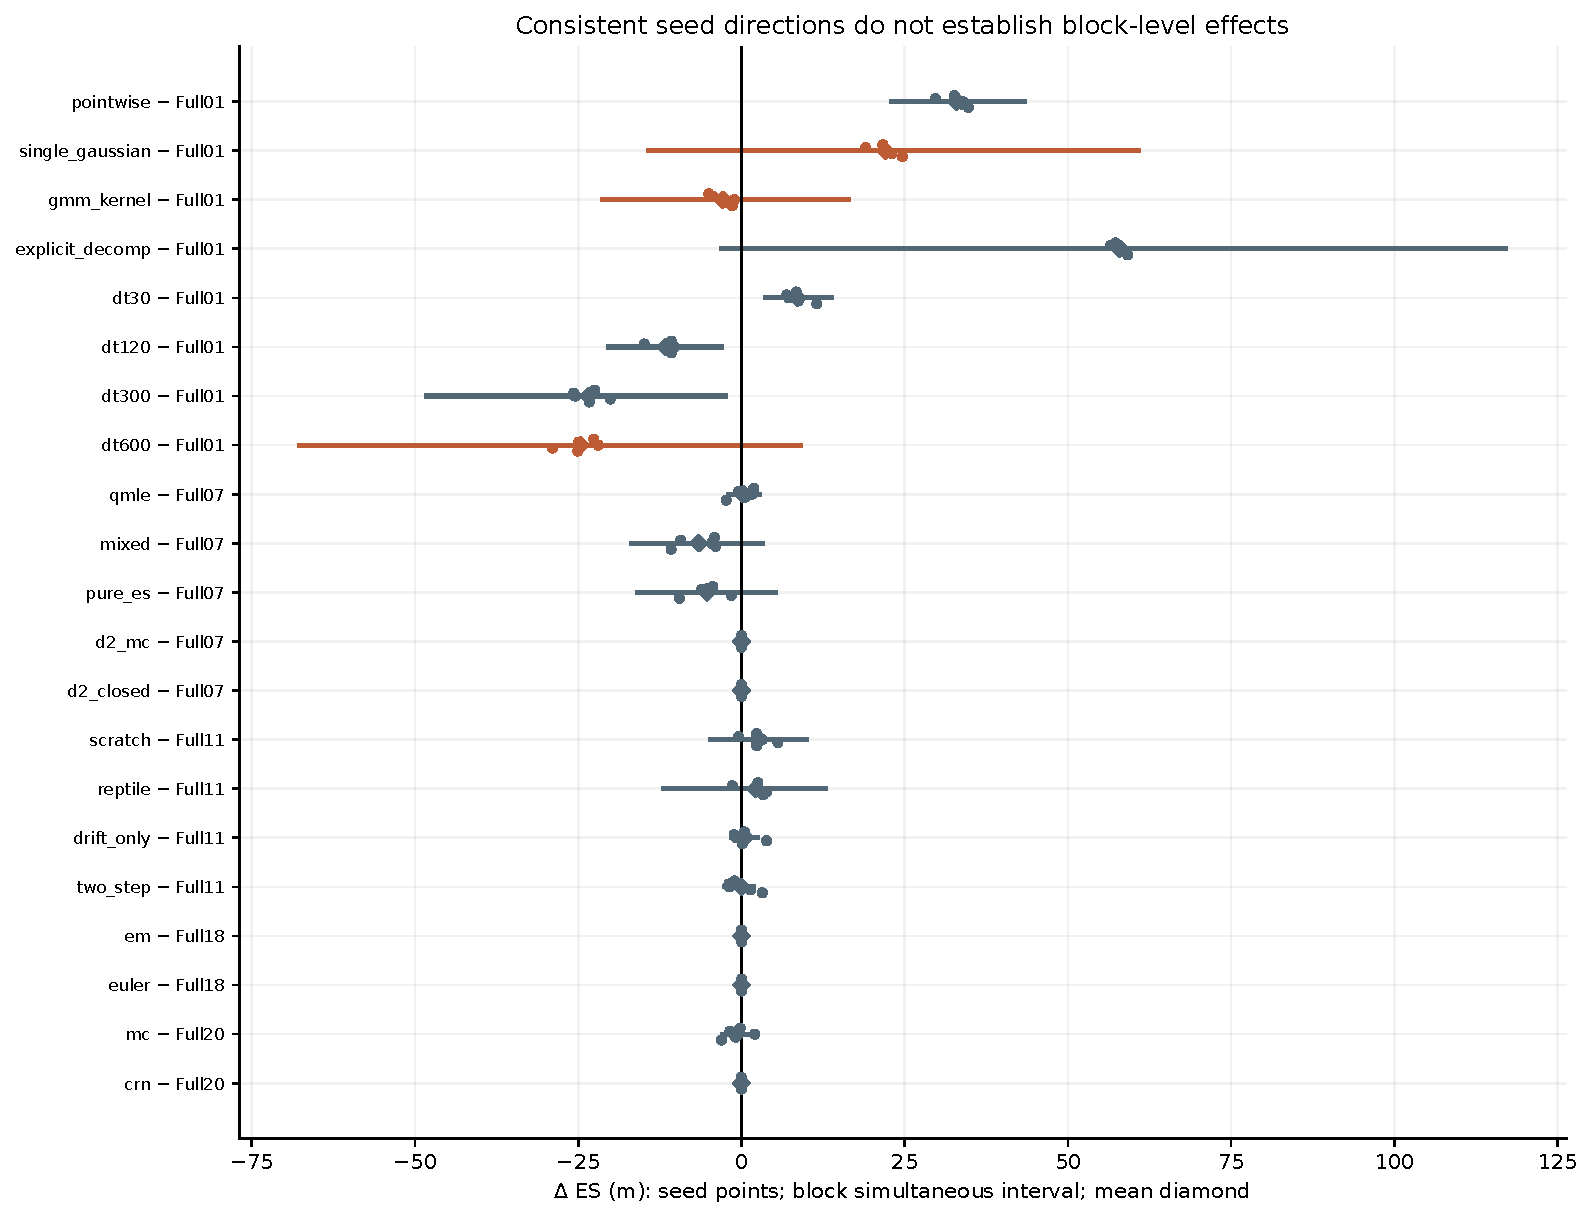
\includegraphics[width=\linewidth]{../figures/revision46-v1/revision46-seeds-and-blocks.pdf}
\caption{五保存种子差值与原记录块同时区间（米）。保留全部比较及种子同号但块区间跨零的例子。
种子只改变Monte Carlo模拟，不代表训练样本或独立参与者重复。}
\label{fig:seed-blocks}\end{figure}
\begin{figure}[htbp]\centering
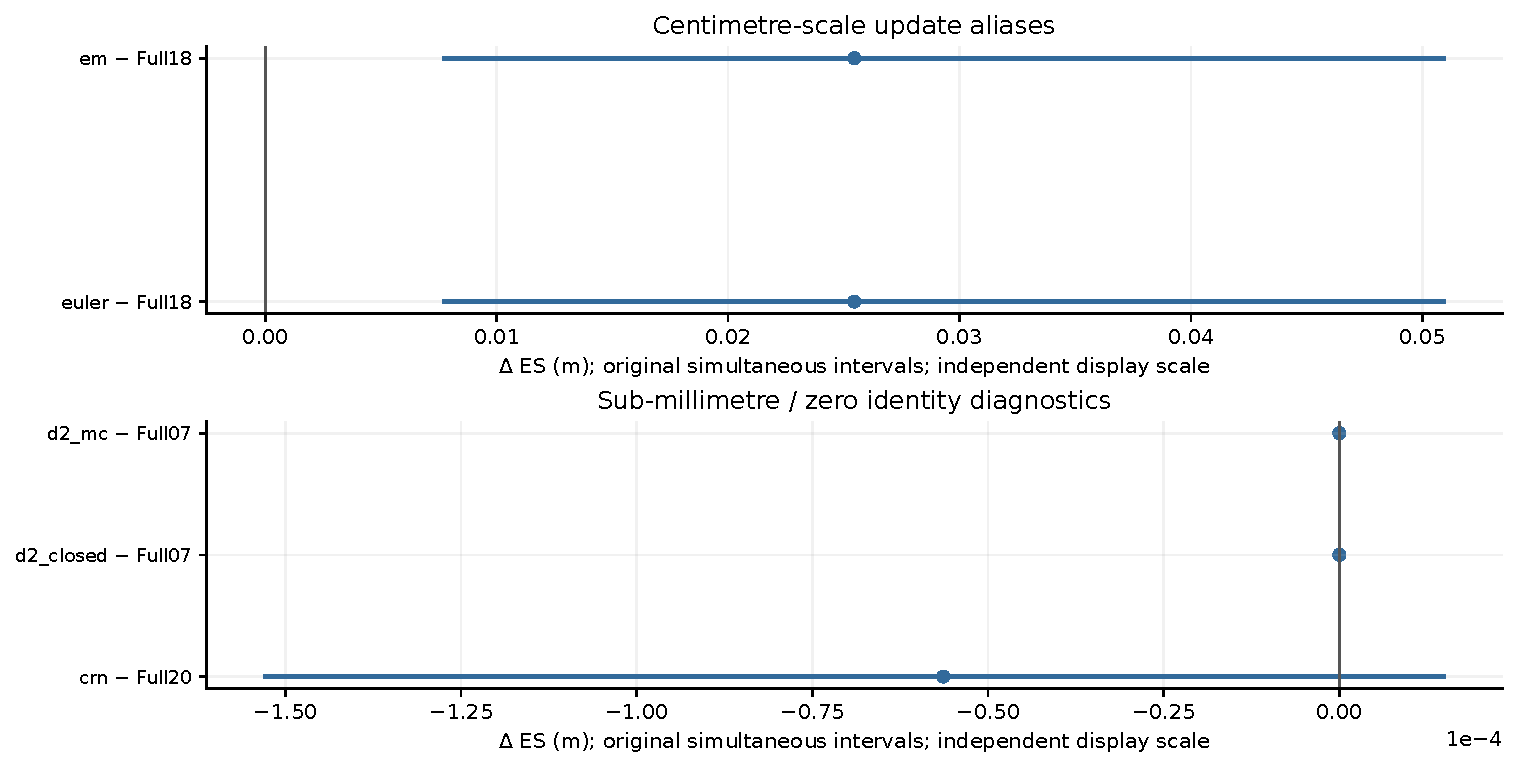
\includegraphics[width=\linewidth]{../figures/revision46-v1/revision46-identity-diagnostics.pdf}
\caption{微小实现一致性差值用明确标注的独立尺度显示，与正文实际效应森林图互补。
原估计和区间不变，零／近零差不提供独立功效证明。}\label{fig:micro-effects}\end{figure}
\FloatBarrier

\section{拟合、成本与完整方法概览}
\begin{figure}[htbp]\centering
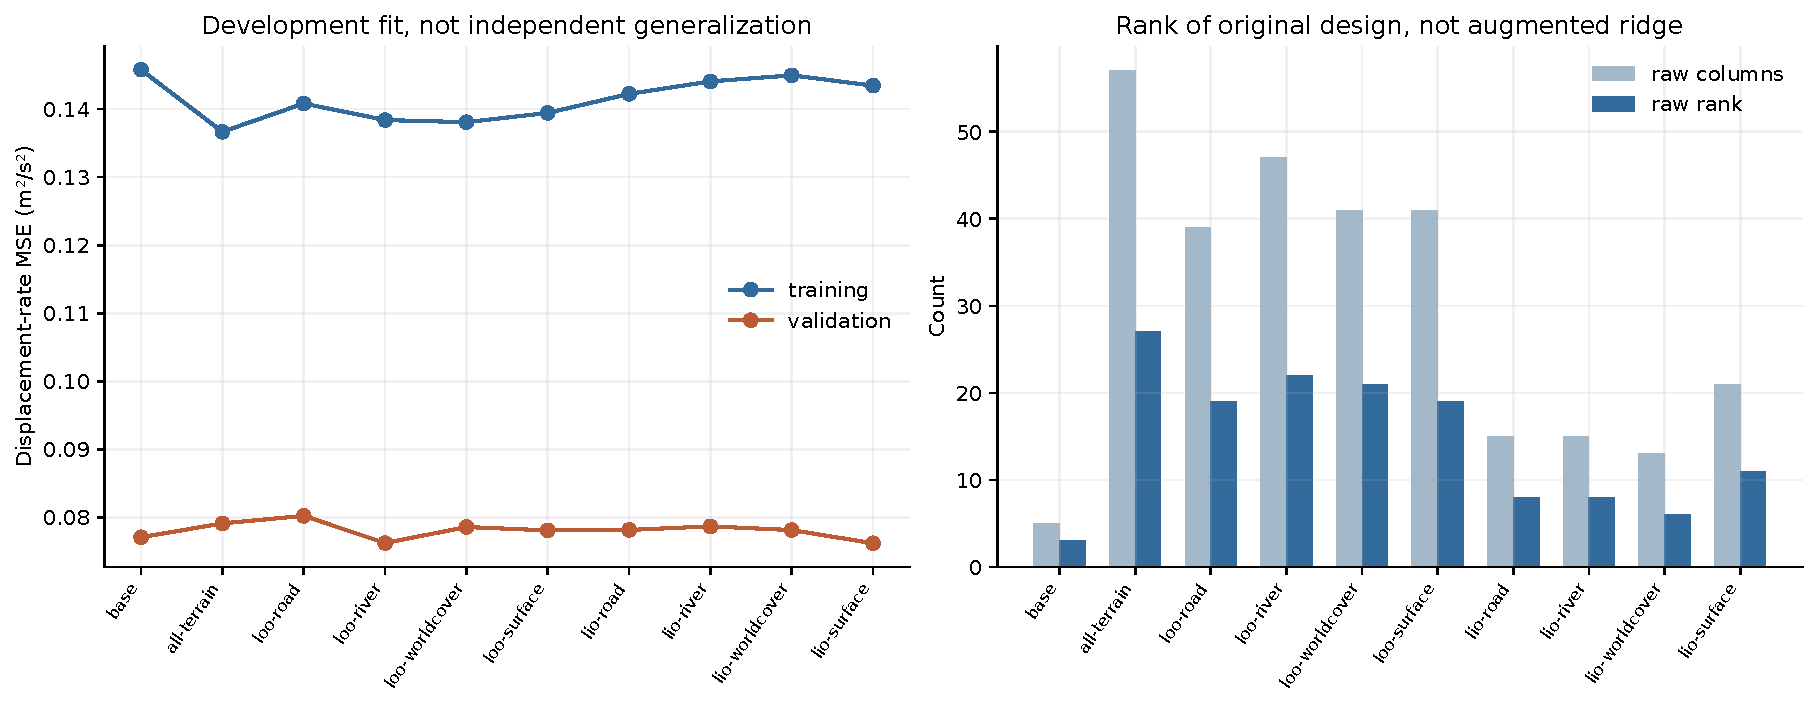
\includegraphics[width=\linewidth]{../figures/revision46-v1/revision46-development-fit.pdf}
\caption{十开发配置训练／验证位移率MSE（米$^2$/秒$^2$）、原始列数与秩。
拟合误差不是预测ES；原始缺秩、增广ridge满秩与样本外表现是不同事项。原行与正则化不变。}
\label{fig:fit-diagnostics}\end{figure}
\begin{figure}[htbp]\centering
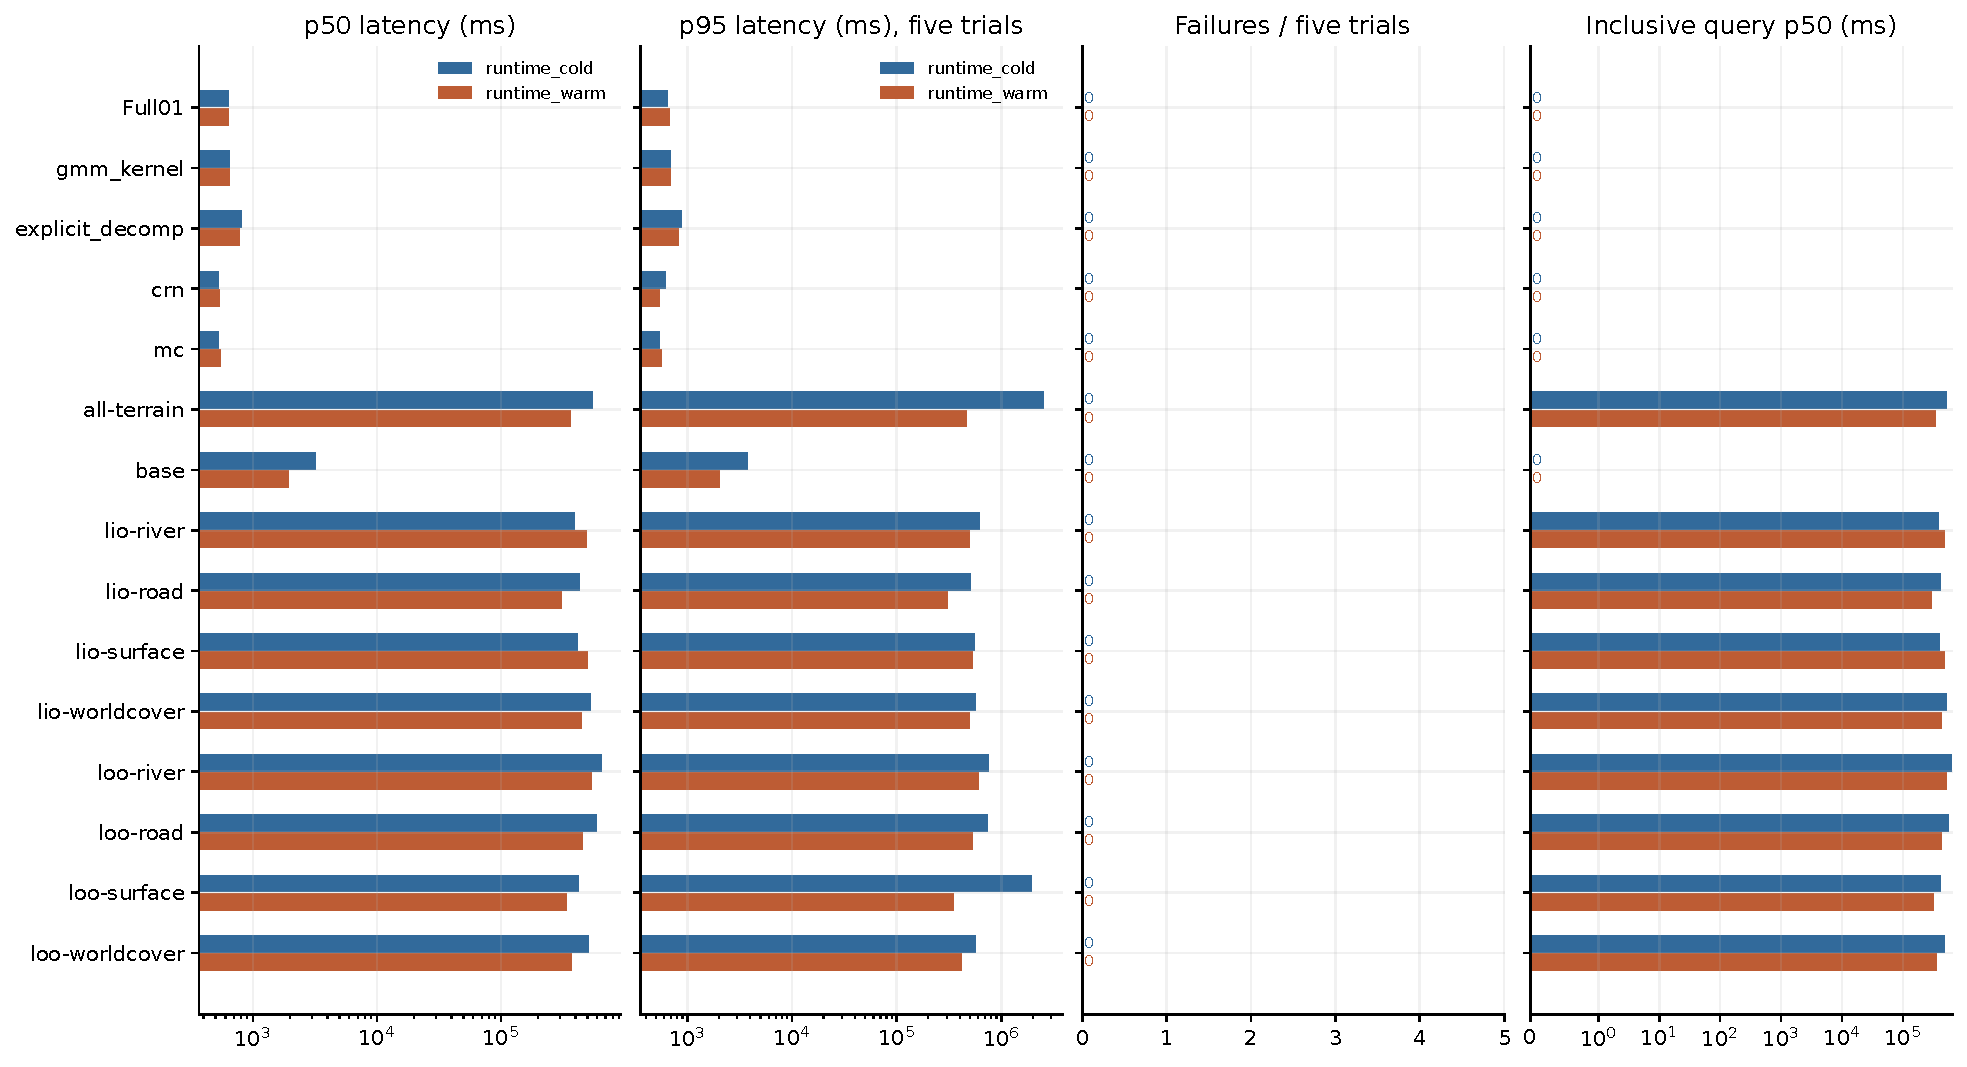
\includegraphics[width=\linewidth]{../figures/revision46-v1/revision46-recorded-runtime.pdf}
\caption{原15对象provider冷／热延迟p50/p95（毫秒）与失败数。
各条件五次，15次预热排除于分位数，而不是排除记录中断暴露试验。
provider冷不是OS缓存冷；查询包含于rollout，五次不估计稳定部署尾延迟。}
\label{fig:runtime}\end{figure}\FloatBarrier
\begin{figure}[p]\centering
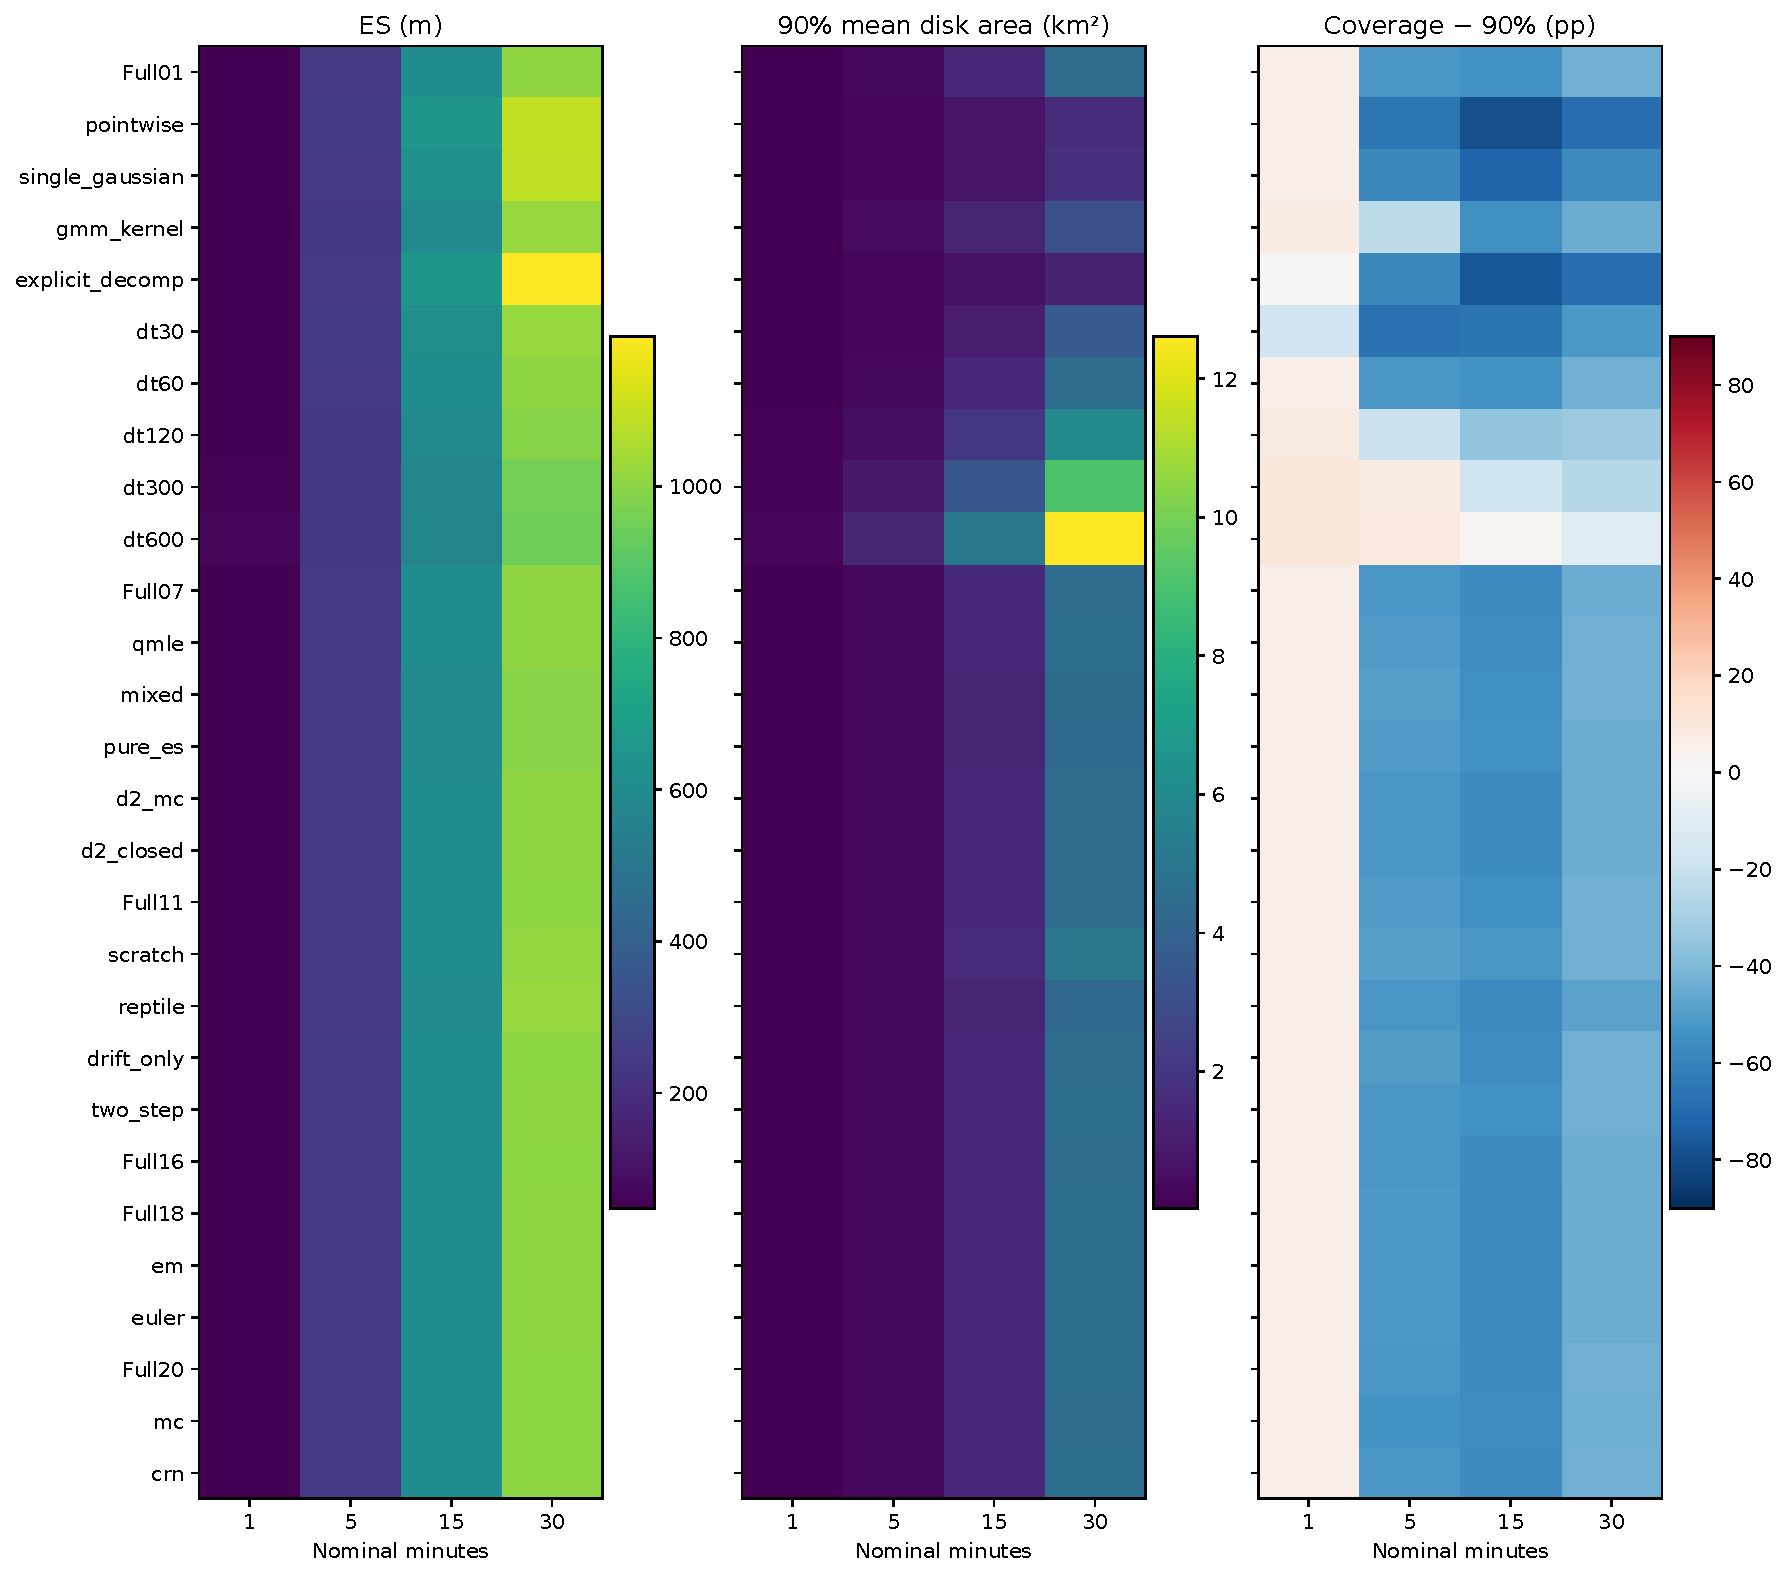
\includegraphics[width=\linewidth,height=.83\textheight,keepaspectratio]{../figures/revision46-v1/revision46-metric-overview.pdf}
\caption{28保存方法身份、四时域：ES（米）、90\%圆平均面积（平方千米）、实际覆盖减名义90\%
（百分点）。统一发散覆盖色阶以零偏差为中心，过覆盖与欠覆盖均可见。
全概率档表继续保留，不选赢家。}\label{fig:method-overview}\hypertarget{fig:method-overview}{}
\end{figure}\FloatBarrier

\section{家族可用性而非地形收益排行榜}
\begin{figure}[htbp]\centering
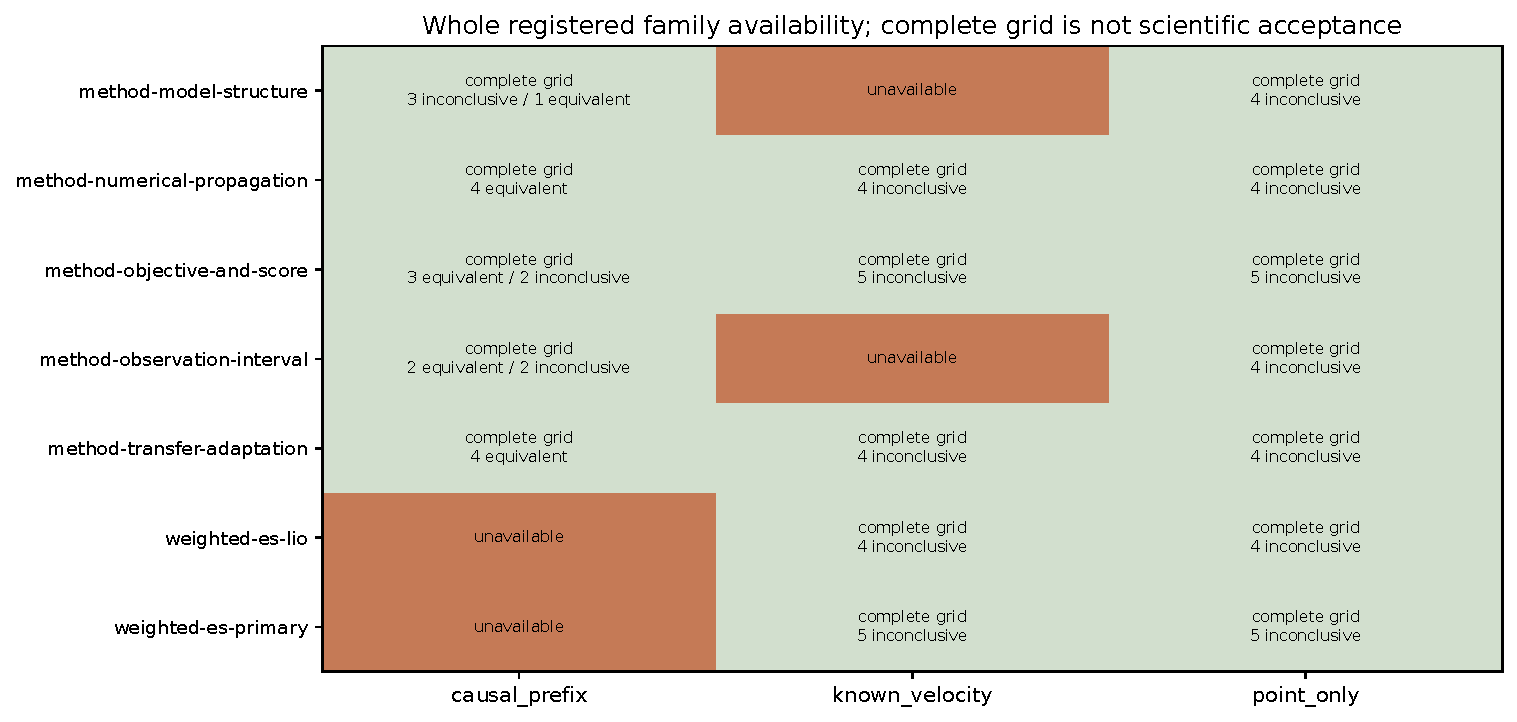
\includegraphics[width=\linewidth]{../figures/revision46-v1/revision46-family-availability.pdf}
\caption{原七家族与三起点模式。必需失败使完整登记家族不可用，成功配对不能替代新家族。
完整不等于接受、实际有益、机制合格或分辨率不变；原比较全表保留具体资格原因。}
\label{fig:availability}\hypertarget{fig:availability}{}\end{figure}\FloatBarrier

\section{缺失输入与历史反馈边界}
在线无效数值零填并加有效性掩码；冻结条件器内漂移变化
$\Delta b=\theta_{\rm num}\Delta f+\theta_{\rm mask}\Delta m$不必为零。
404/81有效开发起点没有覆盖这些缺失状态。
特征文件数、缓存查询数、要素不存在、几何无效和预测失败分别使用不同分母。
全预测早晚速度／漂移序列及逐因素无效率未保存，四位置快照不能恢复它们。
常噪声10秒割线重叠相关一半仅为局部计算，不是完整非线性反馈证据或已拟合观测噪声模型。
本次不重跑长模拟补诊断。

\section{保留的详细科学规格与全量表}
下面机械迁移的单元保留原公式、表格和来源身份。
逐单元哈希与旧标签去向见\path{revision46-source-migration.json}；
改前逐字源稿另以历史名称保留。
仅阅读结构、跨文档链接与计数单位说明改变；当前状态由论文本体说明，
不由旧快照中的等待语气决定。
\section{相关工作与研究范围}\label{sec:related-work}\hypertarget{sec:related-work}{}

\section{连续时间运动与切换动力学}
具有持续性的运动已有成熟的随机模型脉络。Johnson 等对 Ornstein--Uhlenbeck
速度过程积分，得到用于不规则动物遥测的连续时间相关随机游走，并纳入状态空间
观测模型\cite{johnson2008}。与本研究的联系是时间持续性与未来位置分布。
本稿推进的连续状态是位置；速度与方向摘要来自可见前缀，以及启用时的模拟历史，
并未估计相同的潜在速度与观测误差模型。动物遥测是方法上的先例，不是其研究人群
或观测过程与这些 GPX 记录相同的证据。

Ghahramani 与 Hinton 将离散状态和线性连续动力学结合为切换状态空间模型，
对难以精确计算的隐状态后验采用变分推断\cite{ghahramani2000}。
这说明局部高斯动力学不意味着整条轨迹服从单一高斯分布。本稿的拟合模式与条件
传播采用这一类建模思路，但普通方法的模式权重是保存的拟合参数，不是重新根据
当前前缀推断的后验。后文给出本稿具体的拟合、切换与传播规则；混合与切换机制
本身不作为新发明。


\section{环境条件与可学习动力学}
环境信息并不只能以地图图像进入模型。整合步长选择分析同时估计运动与资源选择
参数，将已观测步与可用候选步比较\cite{avgar2016}；其参数表达的勘误另有记录
\cite{avgar2017correction}。这里仅借助该框架定位研究问题，不使用其似然或系数公式。
本稿的道路、河流、覆盖与坡面特征则修正位置 SDE 的漂移；地形对比考察固定特征族
内重拟合后的增量预测信息，而不是栖息地偏好或地景对行为的因果效应。

神经 SDE 扩展了函数表示能力，但学习任务不同。Kidger 等以布朗运动为输入，经 SDE
求解器生成路径，用神经受控微分方程判别器进行 Wasserstein-GAN 训练\cite{kidger2021}。
Gao 等的 Langevin Graph Network Approach（LaGNA）则以恢复耦合网络动力学方程为目标，
用神经模块区分自身、相互作用与扩散贡献\cite{gao2024}。生成路径分布和恢复网络的
支配方程是不同目标。本稿的单记录 GPX 任务评价有限位置预测，不识别主体间相互作用
定律，也不以已知真实方程核验所恢复的动力学。Social GAN 结合循环运动历史、个体间信息汇聚与
对抗多样性\cite{gupta2018}；Trajectron++ 则结合概率性多主体预测、动力学与语义地图
等异构背景\cite{salzmann2020}。这些研究连接了多模态、动力学与环境，但数据、
交互结构和学习目标各有不同。

本研究保留此前选定的线性参数条件修正器，使特征定义与成对组件改动可以检查。
这是固定的表示选择，不是线性模型最优的证据。高斯混合模式、历史反馈和空间特征
也意味着系数线性并不等于整条路径全局线性或单一高斯。本稿的贡献是在同一可见前缀
GPX 任务内，系统比较方法组件和环境输入并报告局限，而不是提出新的神经网络架构。
上述外部模型没有作为本次执行基线；登记的简单惯性参考已有同人群描述性对比，
见第~\ref{sec:inertial-primary} 节。这不是独立核验后的优越性结论，
也不能证明优于所引用的外部模型。


\section{分布评价与有限计算证据}
预测器应作为分布评价，而不只比较均值与实际终点的距离。恰当评分规则提供了这一
基础\cite{gneiting2007,gneiting2008}。本稿将统一的 energy-score 估计器与均值位置误差、
经验覆盖率及区域大小并列报告：更大的区域可能覆盖更多结果，却不改善位置精度。
因此组件效果需要配对比较和明确的实际意义界，而不是对孤立分数排序。

数值积分与集合采样分别引入近似误差\cite{kloeden1992}；增加粒子不会增加记录块数量。
本稿将有限数值证据与块间不确定性分开报告。族内同时置信区间采用 studentized
块 bootstrap\cite{davison1997}，Holm 调整处理的则是零假设检验概率
\cite{holm1979}；适应过程按实际执行的一阶 Reptile 式更新描述\cite{nichol2018}。
这些区分界定了现有比较的支持范围，不能把有限检查写成收敛定理，把置信区间写成
检验概率，或把训练诊断写成留出预测性能。


\section{预测模型与地形归属}
图~\ref{fig:model-data-flow} 先区分实际执行的两套模型，再给出各自方程。
两者都预测未来位置，而不预测未来地图。静态地理特征进入地形分支；普通方法 Full 使用
局部位置、太阳高度及采样模式，并不是地形回归。共用评分协议不意味着它们是同一个
拟合模型，也不意味着其对照可以混用。
\begin{samepage}
\paragraph{术语约定。}
地形条件器（conditioner）指加性漂移修正 \(c_{\theta_g}(F_g)\)，不是独立似然或神经网络；
特征提供器（provider）返回地图或时钟特征；模拟集合（ensemble）是多条预测路径，
不是独立观测样本。裁定（verdict）是登记规则下的证据处置，不是模型排名。
\texttt{Full} 专指普通方法参考，\texttt{base} 与 \texttt{all-terrain} 专指地形配置，
其代码身份保留不译。\texttt{dt} 是观测间隔而非积分步长；
\texttt{two\_step} 与 \texttt{explicit\_decomp} 是两个不同实现，不能混称。
\par
\end{samepage}
\begin{figure}[p]
\centering
\begin{tikzpicture}[
  box/.style={draw=black!65,rounded corners=2pt,align=center,
    font=\small,inner sep=6pt},
  branch/.style={box,text width=7.05cm,minimum height=1.8cm},
  wide/.style={box,text width=15cm,minimum height=1.1cm},
  flow/.style={-{Stealth[length=2.3mm]},thick}]
\node[wide,fill=black!4] (origin) at (0,0)
  {\textbf{起点允许看到的信息}\par
  历史位置及保留时钟；起点模式决定初始运动信息的可用范围。};
\node[branch,fill=blue!5] (method) at (-4,-2.7)
  {\textbf{方法实验：28 个必需配置}\par
  已保存的模式拟合 $\Theta_m,Q_m,\pi_m$；普通 Full 特征
  $\psi=(1,X_e,X_n,S)$，$S$ 为太阳高度。\par
  分别比较结构、观测、拟合与传播策略。};
\node[branch,fill=green!5] (terrain) at (4,-2.7)
  {\textbf{地形实验：10 个配置}\par
  已保存的基线 $B_0$、条件器$\theta_g$、扩散 $L_g$。\par
  在每个当前预测位置查询静态道路、河流、覆盖及坡面；
  数值与有效性掩码共同组成 $F_g$。};
\node[branch,fill=blue!5,minimum height=2cm] (mdyn) at (-4,-5.8)
  {\textbf{模式条件下的位置动力学}\par
  $dX=\Theta_m^\top\psi\,dt+L_m\,dW$，$Q_m=\tau R_m$。\par
  模式策略和历史使用登记间隔 $\tau$；Full 的 $\tau=60$ 秒。
  速度特征只进入显式特征路线，不进入普通 Full。};
\node[branch,fill=green!5,minimum height=2cm] (tdyn) at (4,-5.8)
  {\textbf{历史加地形的位置动力学}\par
  $dX=\{b_0(Z)+c_{\theta_g}(F_g)\}\,dt+L_g\,dW$。\par
  $Z$ 是导出的因果历史，并非独立拟合的速度 SDE；
  历史缓冲区每 5 个模型时钟秒更新。};
\node[wide,fill=black!4] (output) at (0,-8.6)
  {\textbf{每个配置独立保存的预测集合}\par
  $N=512$ 条模拟路径；最大积分步长 $h=5$ 秒；名义预测时长
  $H=1800$ 秒；推进至最后实际目标，在约 1、5、15、30 分钟保存输出。};
\node[wide,fill=orange!7,minimum height=1.6cm] (score) at (0,-11.1)
  {\textbf{评分、聚合，再在登记比较族内配对比较}\par
  分布 ES、均值位置误差与覆盖率；每块先平均 5 个 RNG 种子，再比较记录块。\par
  方法主组阶段统计：$28\times46\times5=6440$ 项预测；
  全部起点模式的方法及地形清单共 $11020$ 项。};
\node[wide,fill=red!4] (truth) at (0,-13.6)
  {\textbf{保留的未来观测：只用于评估}\par
  按登记时钟容差匹配原目标位置；它们不进入预测历史或地形查询回调。};
\draw[flow] (origin.south) -- ++(0,-.25) -| (method.north);
\draw[flow] (origin.south) -- ++(0,-.25) -| (terrain.north);
\draw[flow] (method) -- (mdyn);
\draw[flow] (terrain) -- (tdyn);
\draw[flow] (mdyn.south) -- ++(0,-.25) -| (output.north);
\draw[flow] (tdyn.south) -- ++(0,-.25) -| (output.north);
\draw[flow] (output) -- (score);
\draw[flow] (truth) -- (score);
\end{tikzpicture}
\caption{实际模型及评估的数据流，不是新增实验或神经网络结构。两分支的拟合模型与对照
各自独立；未来观测的箭头只到评分端。$\tau$（观测／历史间隔）、$h$（积分步长）和
$H$（预测时长）不同；$N$ 和五个 RNG 种子是模拟资源，不是独立受试者。
名义时间轴以保留时钟的来源限制为前提。}
\label{fig:model-data-flow}\hypertarget{fig:model-data-flow}{}
\end{figure}

\section{因果地形动力学}
预测目标是给定可见起点后的未来位置分布，不是预测地形，也不是另行预测可观测的未来速度。
\(X_t=(X_{t,e},X_{t,n})^\top\in\R^2\) 是起点锚定的东西/南北位置，单位为米。
\(Z_t\) 包含因果位置历史缓冲、其割线速度 \(v_t\)（米/秒）、单位历史方向 \(h_t\)
及方向有效性 \(\eta_t\)。初始化依据可见位置，此后依据预测位置更新；
\(Z_t\) 并没有一套独立拟合的速度 SDE。
静态地图在当前预测 \(X_t\) 处查询，再与历史组合为包含数值和掩码的
\(F_g(X_t,Z_t)=\phi_g\in\R^{2K_g}\)。此处 \(g\) 表示选定地形配置，不是潜在运动模式。
位置动力学为
\begin{equation}
dX_t=\{b_0(Z_t)+c_\theta(F_g(X_t,Z_t))\}\,dt+L\,dW_t.
\label{eq:terrain-sde}\hypertarget{eq:terrain-sde}{}
\end{equation}
\(W_t\in\R^2\) 是分量独立的标准 Wiener 过程，增量协方差为
\(\operatorname{Cov}(W_{t+\Delta}-W_t)=\Delta I_2\)。漂移 \(b_0+c_\theta\) 单位为米/秒，
\(L\in\R^{2\times2}\) 是常数噪声幅度矩阵，单位为米/根号秒；
协方差是 \(Q=LL^\top\)，不是 \(L\) 本身。确定性部分明确写为
\begin{equation}
\begin{aligned}
r(Z_t)&=(1,v_{t,e},v_{t,n},\|v_t\|,h_{t,e},h_{t,n},\eta_t)^\top,\\
b_0(Z_t)&=B_0^\top r(Z_t),\qquad
c_\theta(\phi_g)=\theta^\top(\phi_g^\top,1)^\top.
\end{aligned}
\label{eq:drift-components}\hypertarget{eq:drift-components}{}
\end{equation}
\(B_0\in\R^{7\times2}\) 以强度 \(10^{-6}\) 的 ridge 拟合基线位移率；
历史方向无效时，两方向分量置零且 \(\eta_t=0\)。
令 \(R\) 的行为 \(r(Z_i)^\top\)，\(V_i=\Delta x_i/\Delta t_i\)，实际第一阶段为
\begin{equation}
B_0=\arg\min_B\{\|RB-V\|_F^2+\rho\|B\|_F^2\}
 =(R^\top R+\rho I_7)^{-1}R^\top V,\qquad\rho=10^{-6}.
\label{eq:baseline-fit}\hypertarget{eq:baseline-fit}{}
\end{equation}
这是未归一化的平方和目标，截距也受惩罚；\(\rho\) 不是均方损失下的惩罚强度。
两阶段依次求解，不联合优化 \(B_0\) 与 \(\theta\)。十个保存的地形拟合具有完全相同的
\(B_0\) 系数，各自的修正设计与扩散参数不同。此处只比较已有参数，没有重新拟合，
也不意味着修正项与历史特征正交。
\(\theta\in\R^{(2K_g+1)\times2}\) 包含截距，拟合基线留下的残差，而非直接以地形标签回归位置。
训练转移 \(i\) 的目标为 \(y_i=\Delta x_i/\Delta t_i-b_0(Z_i)\)，
设计行为 \(x_{{\rm aug},i}=(\phi_{g,i}^\top,1)\)。堆叠得到
\(Y\in\R^{n\times2}\)、\(X_{\rm aug}\in\R^{n\times(2K_g+1)}\)，求解
\begin{equation}
\min_\theta\frac{1}{2n}\|X_{\rm aug}\theta-Y\|_F^2
 +\frac{\lambda}{2}\|\theta\|_F^2,\qquad\lambda=10^{-4}.
\label{eq:conditioner-fit}\hypertarget{eq:conditioner-fit}{}
\end{equation}
第一项对 \(2n\) 个标量输出求均方残差，Frobenius 范数平方是各元素平方和；
第二项惩罚大系数以稳定相关特征设计，偏置也正则化。
\(\lambda\) 已冻结，并非根据最终结果选择。float64 增广最小二乘实现该目标，记录平稳性及条件数。
两个输出时，正规方程为
\((X_{\rm aug}^\top X_{\rm aug}+n\lambda I)\theta=X_{\rm aug}^\top Y\)。
\(n=404\) 时保存的对角惩罚为 \(0.0404\)，不是 \(10^{-4}\)。因此基线与修正项的
正则化具有不同损失归一化，不能直接比较两者数值强度。
每个合格开发窗口只提供起点到首未来观测的一个转移。两层回归对位移率行等权，
不按时长、逆噪声、记录块或参与者加权。实际间隔 \(\Delta t_i\) 可变，
既不是方法拟合间隔 \(\tau\)，也不是积分步长；表~\ref{tab:terrain-fit-intervals}
给出原开发分布，没有规则时间重采样。
这是固定工程特征上的线性参数模型，没有隐藏神经层；但漂移不一定对位置线性，
因为最近地图查询、对数距离、覆盖指示和历史更新依赖预测状态，可能非线性或不连续。
系数正负不受道路吸引等物理规律约束。消融检验的是此模型中的预测增量，不是地形普遍因果效应。
扩散协方差依据训练位移残差估计：
\begin{equation}
LL^\top=\frac1n\sum_{i=1}^{n}
\frac{(\Delta x_i-\widehat b_i\Delta t_i)(\Delta x_i-\widehat b_i\Delta t_i)^\top}{\Delta t_i}.
\label{eq:diffusion}\hypertarget{eq:diffusion}{}
\end{equation}
残差 \(e_i=\Delta x_i-\widehat b_i\Delta t_i\) 是未解释的位移。
冻结漂移的 Brownian 近似下，\(e_i\sim\mathcal N(0,Q\Delta t_i)\)，因此
\(e_i/\sqrt{\Delta t_i}\) 的协方差为 \(Q\)，单位平方米/秒，解释了上式除以时间的归一化。
这不是非线性历史依赖路径的全局似然证明。
等价地，令位移率残差 \(\zeta_i=\Delta x_i/\Delta t_i-\widehat b_i\)，则
\begin{equation}
Q=\frac1n\sum_{i=1}^n\Delta t_i\zeta_i\zeta_i^\top.
\label{eq:terrain-rate-Q}\hypertarget{eq:terrain-rate-Q}{}
\end{equation}
与等行权重的漂移回归不同，此位移率外积含时长因子。残差不再次中心化，分母为
\(n\)，不作自由度校正。这是拟合漂移后的代入二阶矩，不是无偏估计，
也不是漂移与扩散的联合最大似然拟合。
由 \(Q=U\operatorname{diag}(\lambda_1,\lambda_2)U^\top\)，取
\(L=U\operatorname{diag}(\sqrt{\max(\lambda_j,0)})\)。
保存地形模型的加载器拒绝最小特征值低于 \(-10^{-10}\) 平方米/秒或非对称误差
超过绝对容差 \(10^{-12}\) 平方米/秒的矩阵；仅容差内的负舍入在平方根中置零，
不加正值下限或 jitter。十个保存矩阵均对称且严格正定，未发生此截断。
这两个绝对阈值不同于方法分支的相对 PSD 规则；正定不代表预测校准。
每个地形配置保留相同的基线系数，拟合自己的修正列、条件器和扩散参数。
确定性拟合参数可以绑定到多个预测种子，但不因此成为五次独立训练。
断点继续使用保存的十个地形拟合和十六个方法拟合身份。

Euler--Maruyama 以最大 5 秒步长和 512 粒子推进式~\eqref{eq:terrain-sde}。
对单步 \(\Delta\) 及独立 \(\xi_k\sim\mathcal N(0,I_2)\)，实际位置更新为
\begin{equation}
X_{k+1}=X_k+\{b_0(Z_k)+c_\theta(F_g(X_k,Z_k))\}\Delta+\sqrt{\Delta}\,L\xi_k.
\label{eq:terrain-update}\hypertarget{eq:terrain-update}{}
\end{equation}
这将漂移对应到条件平均位移，将扩散对应到增量协方差 \(Q\Delta\)。
预测状态历史有独立的 5 秒模型节拍，每个节拍加入预测位置并重算割线速度。
节拍之间历史和速度固定，地形仍在当前预测位置查询。查询回调没有目标轨迹容器。
历史算子是模型的一部分，不是积分实现细节。地形节拍为起点后的 \(t_j=5j\) 秒。
粒子 \(p\) 追加新预测位置并至多保留三项后，其缓冲记为
\(\{(s_{j,r},x^{(p)}_{j,r})\}_{r=1}^{q_j}\)，\(2\le q_j\le3\)，速度更新为
\begin{equation}
v^{(p)}_{t_j}=\frac{x^{(p)}_{j,q_j}-x^{(p)}_{j,1}}
                        {s_{j,q_j}-s_{j,1}}.
\label{eq:terrain-history}\hypertarget{eq:terrain-history}{}
\end{equation}
初始缓冲只含起点模式允许的可见信息。早期更新可能同时保留非等间隔的原始前缀点
与预测节拍，分母采用实际保留的时间跨度，不能一律写成 5 秒。
当缓冲含三个等间隔节拍位置时，该割线跨越 10 秒。中间积分子步和评分输出本身
不追加历史；历史节拍之间缓冲与速度保持固定。
无效特征数值置零，同时添加有效性列，并保存无效查询数量。


\section{观测历史与模拟历史不是同一种输入}
\label{sec:history-feedback}\hypertarget{sec:history-feedback}{}
地形历史是三位置缓冲，先由观测位置初始化，再按每5秒模型时钟节拍加入生成位置。
若最后一个观测间隔为\(d\)，第一次更新保留最后两个观测点及新位置，割线跨度为\(d+5\)秒；
第二次更新保留起点及第5、10秒位置，之后跨度均为10秒。
因此固定点数并不等于固定割线时长，也不等于输入分布不变。
观测训练、验证及主组前缀的实际时序另列于第~\ref{sec:empirical-history-timings}~节：
它们描述时钟支持，不是测得的反馈速度，也不是改变节拍的实验。

\begin{samepage}
噪声分布也发生改变。仅以常数 \(b,L\) 的局部模型
\(dX_t=b\,dt+L\,dW_t\) 说明，对跨度 \(T>0\) 的割线有
\begin{equation}
\widehat v_t=\frac{X_t-X_{t-T}}{T}
=b+\frac{L(W_t-W_{t-T})}{T},\qquad
\operatorname{Cov}(\widehat v_t)=\frac{Q}{T},\quad Q=LL^\top .
\label{eq:secant-local-noise}\hypertarget{eq:secant-local-noise}{}
\end{equation}
\end{samepage}
重叠缓冲重复使用同一布朗增量。在此常系数示例中，间隔 \(s\ge0\) 的两割线满足
\begin{equation}
\operatorname{Cov}(\widehat v_t,\widehat v_{t+s})
=\frac{(T-s)_+}{T^2}Q .
\label{eq:secant-overlap}\hypertarget{eq:secant-overlap}{}
\end{equation}
因此 \(T=10\) 时，相邻 5 秒地形节拍在有非零方差的方向上相关系数为 \(1/2\)，
不是独立速度噪声。保存的基线与全地形拟合给出
\(\operatorname{tr}(Q)=2.7387,\ 2.5077\ \mathrm{m^2/s}\)，
对应二维局部速度扰动 RMS \(\sqrt{\operatorname{tr}(Q)/10}\)
为 \(0.5233,\ 0.5008\ \mathrm{m/s}\)。
这是现有扩散拟合的算术推论，不是测得的 rollout 速度离散程度，
也不是历史反馈模型的方差界。

GPX 观测坐标还可能带测量误差。若仅以协方差 \(R_{\rm obs}\) 的独立端点误差作说明，
并假定它独立于上述局部过程，则观测割线协方差为 \(Q/T+2R_{\rm obs}/T^2\)。
这不是拟合的传感器模型：本稿既未确定 \(R_{\rm obs}\)，也未证明观测无误差。
模拟则将生成的位置增量重新反馈至基线速度及历史相关特征。方向归一化、地图特征变化
和漂移反馈使常漂移方差式不能代表完整预测器。历史节拍没有速度截断或速度误差滤波。
六份展示案例的原预测档案只保留四个位置输出，没有完整的早期／晚期速度与漂移序列。
因此现有证据不能把历史反馈认定为长期欠覆盖的原因，也未认证异常速度率或改变节拍的
敏感性。方法矩阵使用另一种相邻 \(\tau\) 割线（式~\eqref{eq:method-history}）；
这里的 10 秒计算仅适用于地形缓冲。


\section{冻结地形特征编码}
\label{sec:feature-encoding}\hypertarget{sec:feature-encoding}{}
地形条件器使用冻结的逐点变换，不新增学习式嵌入表征，
也不以最终评估数据重新标准化。对道路、河流，设 \(d_g\) 为查询距离（米），
\(v_g\) 为从查询位置指向选定折线上最近点的东西/南北单位向量。
特征提供器在局部米制投影中确定最近点，并返回到该点的球面距离。
该向量不是道路切线、道路行进方向或河流流向；重合点没有可用方向。数值特征为
\begin{equation}
\ell_g=\log\{1+d_g/(1\,\mathrm{m})\},\qquad
u_g=v_g/\|v_g\|,\qquad g\in\{\mathrm{road},\mathrm{river}\}.
\label{eq:distance-encoding}\hypertarget{eq:distance-encoding}{}
\end{equation}
距离仅在非负时有效；单位向量变换要求范数大于 \(10^{-12}\)。
基线历史方向 \(h\) 使用相同单位向量变换，其可用性仍由因果历史与起点规则决定。
这些选定变换不拟合中心、尺度或截断参数。对数是已冻结的工程选择：保持距离排序、
零距离处有限，并压缩地图距离的大动态范围，导数为 \(1/(1\,\mathrm m+d_g)\)。
这些数学性质解释了表示，但不能证明它最优。当前消融既不确立物理对数响应律，
也没有比较出它优于原始距离；未选变换不属于本次实证结论。

WorldCover 四维指示向量 \(w\) 依次为建筑（代码 50）、植被
（10、20、30、40、95、100）、水体/湿地（80、90）和裸地/雪/其他
（60、70 或其他有限、未识别代码）。末类只适用于可用源值；缺失或 nodata 查询
不重编码成有效的“未知”覆盖。坡面保留提供的六分量
\(s=(\beta,\sin\alpha,\cos\alpha,n_e,n_n,n_u)\)：以弧度计的坡度、
下坡坡向的东西/南北分量及三维表面法向。这是恒等变换，不是另行拟合的地形表示。

对有效覆盖代码 \(k\)，明确定义
\begin{equation}
\begin{aligned}
w_j&=\mathbf1\{k\in\mathcal C_j\},\quad \mathcal C_1=\{50\},\\
\mathcal C_2&=\{10,20,30,40,95,100\},\quad\mathcal C_3=\{80,90\},\\
\mathcal C_4&=\R_{\rm finite}\setminus(\mathcal C_1\cup\mathcal C_2\cup\mathcal C_3).
\end{aligned}
\label{eq:cover-indicators}\hypertarget{eq:cover-indicators}{}
\end{equation}
合并类别不允许分别裁定建筑、各植被类、湿地或雪的效果。
绝对高程 \(H\) 用于导出坡面，不是已选条件器输入列。
设 DEM 东西/南北梯度为 \(\gamma=(\partial_eH,\partial_nH)\)，则
\begin{equation}
\begin{aligned}
\beta&=\arctan\|\gamma\|,\quad (\sin\alpha,\cos\alpha)=-\gamma/\|\gamma\|,\\
(n_e,n_n,n_u)&=(-\gamma_e,-\gamma_n,1)/\sqrt{1+\|\gamma\|^2}.
\end{aligned}
\label{eq:surface-geometry}\hypertarget{eq:surface-geometry}{}
\end{equation}
特征提供器用 DEM 邻点的中心差分估计梯度。\(\alpha\) 从正北顺时针计，指向下坡。
平地没有几何定义的坡向，特征提供器明确使用 \((0,0)\) 坡向向量，不能将其解释为朝北。
因此平地的方向组合可为零，并不证明真实运动与坡向垂直；掩码仍依据源有效性。

四个选定组合严格为
\begin{align}
c_{\rm road}&=\ell_{\rm road}u_{\rm road},&
c_{\rm river}&=\ell_{\rm river}u_{\rm river},\notag\\
c_{\rm cover}&=\ell_{\rm road}w,&
c_{\rm surface}&=(h^\top a,\ h^\top q),
\label{eq:feature-compositions}\hypertarget{eq:feature-compositions}{}
\end{align}
其中 \(a=-(\sin\alpha,\cos\alpha)\) 是上坡方向，
\(q=(-a_n,a_e)\) 是在东西/南北坐标中将上坡方向正向旋转 90 度的等高线方向。
上坡只有一个方向，反向是下坡，不是第二种登高方向。
等高线有两个朝向，选定 \(q\) 固定符号约定，换成 \(-q\) 会改变 \(h^\top q\) 的正负。
\(h^\top a>0\) 表示向上坡对齐，负值表示向下坡；带符号的等高线投影区分两个朝向，
不意味着其中一个有先验物理优势。坡面组合因此只增加两个方向投影，
不是六维坡面与二维历史的全部十二个乘积，也不再将投影乘以坡度大小。
道路、河流、覆盖和坡面组合分别增加 2、2、4、2 列，加上 18 个选定基础变体列，
全地形模型共 28 个数值列。

一个变体只有在所需规范输入均有限且源状态为 \texttt{valid} 时可用，
并须满足上述距离域和向量范数条件。组合掩码要求贡献输入均可用；坡面投影使用
坡向和历史掩码。在线规范数值先表示为 float32，以匹配保存的快照值，再使用
相同变换内核。对数值 \(f_j\) 和布尔掩码 \(m_j\)，条件器输入为
\begin{equation}
\phi=(\widetilde f_1,\ldots,\widetilde f_K,m_1,\ldots,m_K)^\top,
\qquad \widetilde f_j=
\begin{cases}f_j,&m_j=1,\\0,&m_j=0,\end{cases}
\label{eq:feature-masks}\hypertarget{eq:feature-masks}{}
\end{equation}
全地形的 \(K=28\)。无效值通过掩码保留，不丢弃，也不解释为实测零值。
全部 LOO/LIO 配置复用这些冻结变换，仅改变选取列和独立拟合的动力学。


\section{方法动力学与登记备选模型}
\label{sec:method-model}\hypertarget{sec:method-model}{}
方法矩阵是另一个模型族，不是仅给地形回归换列名。给定模式 \(M_t=m\)，局部动力学为
\begin{equation}
\begin{aligned}
dX_t&=b_m(X_t,Z_t,S_t)\,dt+L_m\,dW_t,\\
b_m&=\Theta_m^\top\psi(X_t,Z_t,S_t),\quad L_mL_m^\top=Q_m=\tau R_m.
\end{aligned}
\label{eq:method-sde}\hypertarget{eq:method-sde}{}
\end{equation}
\(S_t\) 为几何太阳高度角，\(\psi\) 通常包含 \((1,X_{t,e},X_{t,n},S_t)\)，
\(\Theta_m\) 是模式专属 ridge 系数，\(R_m\) 为拟合的速度率残差协方差，\(\tau\) 为观测/训练间隔。
冻结系数的 Euler 单步条件分布为 \(\mathcal N(X_t+b_m\Delta,Q_m\Delta)\)。
以三个模式概率 \(\pi_m\) 初始化未观测模式，第一步给出混合
\(\sum_{m=1}^3\pi_m\mathcal N(X_t+b_m\Delta,Q_m\Delta)\)。
段内固定模式保留该抽样；pointwise-mixture 与 GMM-kernel 路线在 \(\tau\) 节拍重新抽样。
single-Gaussian 和显式特征路线只有一个模式；后者向 \(\psi\) 添加速率和径向方向两分量。
太阳条件非线性和采样模式历史意味着多步预测并不保证是精确的三高斯密度。
所有执行拟合仍对特征系数线性，没有执行神经网络基线；混合模型名称与实际训练划分规则如下区分。

\paragraph{哪些可见输入实际影响预测？}
普通 Full、逐点混合、单高斯及 GMM-kernel 路线使用
\(\psi=(1,X_e,X_n,S)\)，不使用给定速度或带符号的历史方向作为特征。
基础拟合中 \(\pi_m=n_m/\sum_k n_k\)，其中 \(n_m\) 是分配到模式 \(m\) 的训练转移数。
Full 保存混合后的参数
\(\pi_m=0.35\pi_m^{\rm pretrain}+0.65\pi_m^{\rm adapt}\)。
预测读取保存的概率，不依据新的可见前缀估计
\(\Pr(M_0=m\mid\text{新可见前缀})\) 后验，也不从最终评估前缀重拟合系数或概率。
因此，固定数值位置、时钟、条件场、保存参数及随机流身份后，仅改变初始速度，
上述普通路线的预测不变。更新速度缓冲并不能证明普通 Full 使用了速度特征。

这条依赖关系不等于丢弃全部可见位置。主要方法模式的坐标系以首个可见点为锚，
决定数值起点 \(X_0\) 及太阳条件场使用的地理转换；两个次要模式改用预测起点坐标系，
避免给 point-only 带入隐藏前缀。因此，即使最后地理位置固定，改变前缀仍可能改变
数值位置或坐标系；不同起点身份还选择不同随机流。
次要模式比较不能隔离上述固定输入条件下的速度敏感性。
显式特征路线增加速率 \(\|v\|\) 和位置径向方向
\(X/\max(\|X\|,10^{-9})\)，在 \(X=0\) 时方向为零；单独反转速度不改变速率。
地形模型则通过 \(b_0\) 和保留特征直接使用速度及历史方向。
固定坐标系与随机流的合成反向前缀测试在四个短时输出检查上述区别，
不是新增实证预测，也不是最终矩阵的独立审计。
必需配置比较模式结构、显式分解、观测间隔、学习目标、训练/适应和数值推断。
必需 Full 模型保留太阳条件，但替代条件 arm 已豁免，不能据此裁定太阳条件的效果。
方法噪声使用速度率残差协方差 \(R\)，保留时间坐标下的增量协方差为 \(Q=R\tau\)，
其中 \(\tau\) 为登记训练/观测间隔，不能替换为积分步长。方法历史也跟随登记间隔。
重复 Full 锚点保留配置身份，但不当成新的独立重复。
具体而言，方法历史节拍 \(t_j=j\tau\) 上逐路径的速度更新为
\begin{equation}
v^{(p)}_{t_j}=\frac{U^{(p)}_{j\tau}-U^{(p)}_{(j-1)\tau}}{\tau},\qquad
U^{(p)}_t=\begin{cases}
X^{(p)}_t,&\text{MC 或 CRN},\\
\mu^{(p)}_t,&\text{条件高斯矩传播}.
\end{cases}
\label{eq:method-history}\hypertarget{eq:method-history}{}
\end{equation}
位置及条件中心 \(\mu^{(p)}_t\) 均使用方法自身坐标系；中心以该抽样模式路径为条件，
不是集成均值。首次更新以起点作为 \(U^{(p)}_0\)，此前保留起点给定的速度。
这采用相邻节拍割线，不同于式\eqref{eq:terrain-history}的地形历史缓冲。
Full 的节拍为 60 秒，观测间隔变体使用各自的 \(\tau\)。速度通道提供显式特征路线
的速率特征，并非另一条拟合的速度 SDE，也不是普通 Full 漂移的额外输入列。

Full 方法使用三个段内固定模式、太阳高度角、全局预训练和目标适应、energy-score
协方差校准、split 积分及条件高斯矩传播，参考观测间隔为 60 秒。
五个登记家族包含 21 个候选与 Full 比较（表\ref{tab:method-families}）；另六个
Full 锚点和相同的 60 秒 replay 构成其余七个必需槽，不增加独立对照数量。

\begin{table}[htbp]
\centering\small
\caption{登记的主要方法比较；不包含最终实证裁定。数量为候选配置数，不是记录块数。}
\label{tab:method-families}\hypertarget{tab:method-families}{}
\begin{tabular}{p{.21\linewidth}p{.63\linewidth}r}
\hline
家族 & 模型变体及对应 Full 参考 & 数量\\
\hline
模型结构 & 逐点混合、单高斯、残差混合、显式特征；Full01 & 4\\
观测间隔 & 30/120/300/600 秒；Full01 & 4\\
目标与评分 & QMLE、mixed、pure energy、二维 MC/闭式评分；Full07 & 5\\
训练及适应 & scratch、Reptile、drift-only、two-step；Full11 & 4\\
数值传播 & 两个 Euler 标签（Full18）、MC/CRN 传播（Full20） & 4\\
\hline
\end{tabular}
\end{table}

\noindent 附录~\ref{sec:method-implementation-map} 将科学名称映射到完整配置清单。
\texttt{dt} 标签为以秒计的观测/训练及历史间隔，不是积分步长或预测时长。
太阳条件、动物迁移及桥过程变体不属于本研究的效果结论；
另行拟合的十配置地形实验仍保留。

\paragraph{模式拟合及特征。}
训练模式按段位移方向排序分为三等份，同值按段身份排序，并非用混合似然 EM 推断的
行为状态。各模式分别拟合含截距、局部位置和太阳高度角的岭回归。
残差混合按 pooled 残差的 east、north、\(-({\rm east}+{\rm north})\) 三项中的最大项分组；
单高斯使用全部转移。显式特征路线也是单模式，增加速度及径向方向的两个分量，
并非单独拟合径向/切向动力学分解。预测时段内模式保持固定，切换路线在参考间隔时钟
重抽模式，不在每个积分子步重抽。太阳高度角由预测位置与保留时钟按模型的 UTC 解释及 NOAA
fractional-year 近似重算\cite{noaa}；采集时钟的 UTC 来源未获独立认证
（第~\ref{sec:clock-and-map-provenance}~节），这里是几何高度角，不是天气测量或折射模型。

\Needspace{14\baselineskip}
\paragraph{基础回归及协方差估计。}
\label{sec:method-base-fit}\hypertarget{sec:method-base-fit}{}
对一个准备批次和分量\(m\)，\(D_m\)含\(n_m\)个特征行，\(Y_m\)为对应二维位移率目标。
基础回归最小化
\(\tfrac12\|D_m\Theta-Y_m\|_F^2+\tfrac\rho2\|\Theta\|_F^2\)，取\(\rho=10^{-6}\)。
全部系数包括截距均受惩罚，数据项不除以\(n_m\)。拟合残差为
\(e_{mi}=y_i-\widehat\Theta_m^\top\psi_i\)，其均值为\(\bar e_m\)，实际基础参数为
\begin{align}
 \widehat\Theta_m&=(D_m^\top D_m+\rho I_d)^{-1}D_m^\top Y_m,
 \label{eq:method-base-ridge}\hypertarget{eq:method-base-ridge}{}\\
 \widehat R_m&=\frac1{n_m-1}\sum_{i=1}^{n_m}
 (e_{mi}-\bar e_m)(e_{mi}-\bar e_m)^\top+\epsilon I_2,
 \qquad \epsilon=10^{-8}.
 \label{eq:method-base-covariance}\hypertarget{eq:method-base-covariance}{}
\end{align}
实现求解线性方程，不显式计算逆矩阵；\(d\)是特征数。样本协方差先对称化，
再添加量纲为\(\mathrm{m}^2/\mathrm{s}^2\)的jitter。方法协方差经过中心化并使用\(n_m-1\)，
不同于地形位移率残差二阶矩；这不是回归自由度修正，也不证明SDE扩散估计无偏。
基础比例为\(\widehat\pi_m=n_m/\sum_k n_k\)。每个分量至少需要两个转移，否则拟合失败，
不合并、删除或替换该分量。这些是基础拟合，不是后续适应／校准参数。
若写成平均损失目标，基础惩罚为\(\rho/n_m\)；归一化Reptile内目标使用的则是\(\rho\)
（式~\eqref{eq:meta-inner}）。相同符号不表示两种程序具有相同的样本数缩放惩罚。

\paragraph{残差混合标签究竟表示什么。}
\label{sec:residual-mixture-fit}\hypertarget{sec:residual-mixture-fit}{}
GMM-kernel路线先在本批次全部转移上拟合同一岭回归，再计算
\(r_i=y_i-\widehat\Theta_{\rm pool}^\top\psi_i\)。分量标签为
\begin{align}
 g_i=1+\underset{j\in\{0,1,2\}}{\operatorname{argmax}}\,
       (r_{i,e},r_{i,n},-r_{i,e}-r_{i,n})_j .
 \label{eq:gmm-residual-partition}\hypertarget{eq:gmm-residual-partition}{}
\end{align}
并列时选上述顺序中首个最大项，零残差因此属于分量1。
随后各组分别按式~\eqref{eq:method-base-ridge}--\eqref{eq:method-base-covariance}
拟合回归及中心化协方差。pooled系数仅用于产生标签，不保留为叠加残差中心的共同漂移。
每个基础拟合批次仅分组一次，训练与适应分别处理；没有迭代似然优化、responsibility或
expectation--maximization。这里GMM指最终高斯混合转移路线，不是标准潜在高斯混合似然拟合。
预测使用保存的混合后概率，在\(\tau\)时钟重抽分量，而非随状态变化的后验responsibility。
原分组成员及转移频数未保存，算法规格不提供其经验频数，也不证明跨批次行为状态匹配。

\paragraph{段方向排序标签。}
具体地，对一个含 \(K\) 段的批次，先按
\(\operatorname{atan2}(X_{\rm end,n}-X_{\rm start,n},
X_{\rm end,e}-X_{\rm start,e})\) 排序，再按段身份处理并列。
以零起算排序位置 \(r_s\)，标签为
\begin{equation}
m_s=\min\{2,\lfloor 3r_s/K\rfloor\},\qquad r_s=0,\ldots,K-1.
\label{eq:segment-rank-mode}\hypertarget{eq:segment-rank-mode}{}
\end{equation}
实现标签 0、1、2 对应前文混合分量序号 1、2、3，即 \(m=m_s+1\)。
排序角以弧度计，采用 \([-\pi,\pi]\) 分支，切口位于向西轴；实现使用
\texttt{math.atan2}，包括其带符号零约定，不做圆周解缠或零位移方向过滤。
该标签是排序划分，不是观测到的运动状态。
同一段的各转移继承该标签。十六份原拟合的角色记账均保留相同的 328 个训练段、
76 个适应段及 81 个验证段。表~\ref{tab:mode-rank-cardinality} 给出该规则在完整角色
批次上确定的段数；不重建方向、残差或拟合。段长不同，所以这些段数不提供逐模式转移数
\(n_m\) 或概率 \(\pi_m\)，也不描述残差混合的分组。各批次独立重新排序，
包括 Reptile 的合格地区任务；本表不是逐地区任务清点，相同模式序号不证明相同物理方向
或行为状态。

\begin{table}[htbp]
\centering\small
\caption{完整准备角色批次的确定性方向排序段数；不是逐模式转移频数、最终混合概率、
GMM 残差组数或 Reptile 地区任务组数。}
\label{tab:mode-rank-cardinality}\hypertarget{tab:mode-rank-cardinality}{}
\begin{tabular}{lrrrr}
\toprule
准备角色 & 段数 & 模式 0 & 模式 1 & 模式 2\\
\midrule
训练 & 328 & 110 & 109 & 109\\
适应 & 76 & 26 & 25 & 25\\
验证 & 81 & 27 & 27 & 27\\
\bottomrule
\end{tabular}
\end{table}

\FloatBarrier
\paragraph{拟合与适应范围。}
训练观测按登记间隔重采样，最多移除一个末端不完整间隔，不改变评分目标。
全局拟合和适应拟合的混合使用 0.65 的适应权重。drift-only 在该混合阶段保留预训练
协方差，而 \texttt{all} 和 \texttt{two\_step} 使用相同的协方差混合；后续验证校准
仍可缩放协方差。因此 two-step 保留执行身份，不代表独立的顺序优化算法。
scratch 只使用适应拟合。Reptile 按适配器的来源地点标签组织开发段，至少两个任务，每任务至少
三段，在相同目标适应混合前执行四个外循环 epoch 和五个内循环梯度步。

任务按来源地点的精确字符串分组，不含国家键、不统一大小写；
这些采集标签不是已核实城市、行政区或独立参与者。
84个标签组中，30组满足至少三段，包含258段、每遍全部合格任务共20,029个转移；
另54组的70段、5,980个转移仍参与全局初始化，但不进入任务访问循环。
附录~\ref{sec:reptile-task-accounting} 给出精确来源字段规则、完整任务表和保存暴露量记账。

\paragraph{实际有限 Reptile 更新。}
初始化为全局训练岭回归。合格标签组按字典序在每个 epoch 各访问一次，不随机抽任务或打乱。
方向三等份在每个标签任务内重新计算，跨任务模式序号不是匹配的行为标签。
任务 \(r\)、模式 \(m\) 的特征、位移率目标和转移数分别记作
\(D_{rm}\)、\(Y_{rm}\)、\(n_{rm}\)。取 \(\rho=10^{-6}\)，五个内步各为
\begin{equation}
\begin{aligned}
L_{rm}&=\|D_{rm}\|_2^2/n_{rm}+\rho,\\
\Theta_m^{k+1}&=\Theta_m^k-\frac{0.5}{L_{rm}}
\left\{\frac{D_{rm}^{\top}(D_{rm}\Theta_m^k-Y_{rm})}{n_{rm}}
                 +\rho\Theta_m^k\right\}.
\end{aligned}
\label{eq:meta-inner}\hypertarget{eq:meta-inner}{}
\end{equation}
这是归一化任务 ridge 目标的全批量梯度下降，不是闭式重求解或 Adam。
初始化 base ridge 使用未归一化平方损失，相同 \(\rho\) 不表示相同有效惩罚。
不足两个转移的模式跳过系数更新并保留原协方差；否则使用更新后中心化残差、分母
\(n_{rm}-1\) 的样本协方差加 \(10^{-8}I\)，模式概率取任务转移比例。
epoch \(e=0,1,2,3\) 每次任务访问后为
\begin{equation}
\xi\leftarrow\xi+\frac{0.35}{\sqrt{e+1}}(\xi_r^{\rm inner}-\xi),
\qquad\xi=(\{\Theta_m\},\{R_m\},\pi).
\label{eq:meta-outer}\hypertarget{eq:meta-outer}{}
\end{equation}
概率重新归一化。任务访问次数相同、外步相同，不按转移数做 pooled 外更新。
协方差和概率插值属于本有限实现，不声称它们是原 Reptile 目标的梯度参数。
目标适应拟合独立求解后混合：
\begin{equation}
\Theta_m^{\rm final}=0.35\Theta_m^{\rm meta}+0.65\Theta_m^{\rm target}.
\label{eq:target-blend}\hypertarget{eq:target-blend}{}
\end{equation}
\texttt{all} 对 \(R_m\)、\(\pi\) 同样混合，再做验证协方差校准。
因此不是从该初始化完全重求目标最优解而抹去其影响。

原保存 Reptile 拟合报告 30 个合格任务，任务访问残差 MSE 内更新前后均值为
1.595 / 1.260，单位平方米/平方秒。这是重复训练任务诊断，不是留出性能或 120 个
独立观测。最终保存的系数、协方差和概率分别与普通 Full 不同。
原结果未保存元更新前及目标混合前的中间参数快照，不通过新增拟合重建。
这些证据说明实际参数流，不证明元学习普遍获益。
保存来源对应与任务记账统一见附录~\ref{sec:reptile-task-accounting}。

\paragraph{有限拟合目标比较实际改变了什么。}
\label{sec:estimator-calibration}\hypertarget{sec:estimator-calibration}{}
以 \(\Theta_m^0,R_m^0,\pi_m^0\) 表示训练和目标适应后、验证校准前的模型。
这里四条路线均在 \(\tau=60\) 秒下使用 26009 个训练、5762 个适应、6149 个验证转移，
分别来自 328、76、81 个窗口。只有 mixed 与 pure-ES 再在验证转移上做一次 ridge 拟合，
得到 \(\Theta_m^V\)，模式标签使用该角色自身的确定性方向三等份。
按相同模式序号混合不证明两次拟合的行为状态匹配。候选参数为
\begin{equation}
\Theta_m(\eta)=(1-\eta)\Theta_m^0+\eta\Theta_m^V,\qquad
R_m(s)=s^2R_m^0,\qquad \pi_m=\pi_m^0 .
\label{eq:estimator-drift-grid}\hypertarget{eq:estimator-drift-grid}{}
\end{equation}
尺度网格为 \(\mathcal S=\{0.55,0.75,1,1.3,1.7\}\)，
漂移混合网格为 \(\mathcal A=\{0,0.1,0.25,0.5\}\)。
不把验证拟合的协方差或模式概率替换到候选中。

验证速度率目标、特征与确定性标签分别为 \(y_i,\psi_i,\ell_i\)，令
\(r_i(\eta)=y_i-\psi_i^\top\Theta_{\ell_i}(\eta)\)。
三分量模型的\(\ell_i=m_{s(i)}+1\)为验证段自身的方向排序标签；单分量模型总选分量1。
残差混合路线的验证代理也使用这些段方向标签，而非残差组标签\(g_i\)：
验证残差程序没有重新分配GMM组或推断混合responsibility。
这个保留的标签不匹配是实现边界，不是匹配分量的混合似然校准。
这里只如实披露，不重新拟合、重标记或修改任何保存预测。
校准使用未按 \(\pi_m^0\) 加权的平均协方差
\(\overline R^0=M^{-1}\sum_mR_m^0\)，并令
\(S_s=s^2\overline R^0+\epsilon I_2,\ \epsilon=10^{-8}\)；
这次 jitter 是各原拟合 \(R_m^0\) 已含 jitter 之外的额外项。
对独立 \(U,U'\sim\mathcal N(0,S_s)\)，两个验证替代目标为
\begin{equation}
\begin{aligned}
E(\eta,s)&=\frac1{n_V}\sum_i
 \left\{\mathbb E\|U-r_i(\eta)\|-\tfrac12\mathbb E\|U-U'\|\right\},\\
N(\eta,s)&=\tfrac12\left\{2\log(2\pi)+\log\det S_s
 +\frac1{n_V}\sum_i r_i(\eta)^\top S_s^{-1}r_i(\eta)\right\}.
\end{aligned}
\label{eq:estimator-validation-surrogates}\hypertarget{eq:estimator-validation-surrogates}{}
\end{equation}
代码二次项使用伪逆；jitter 后协方差为正定。
\(E\) 用每轴 10 阶的张量积 Gauss--Hermite 求积近似。
若 \(g_k,w_k\) 为 100 个二维节点及归一化乘积权重，\(C_sC_s^\top=S_s\)，
两个期望分别用 \(\sum_kw_k\|\sqrt2C_sg_k-r_i\|\) 和
\(\sum_kw_k\|2C_sg_k\|\) 近似。总体式是该高斯速度率替代分布的 energy score
（式~\eqref{eq:population-es}），有限求积本身不证明严格 proper。
它不是最终多模式位置预测或联合路径评分。\(N\) 是固定速度率单位下 pooled 高斯
密度的负对数，不是混合似然或连续时间 SDE 的似然。

记 \(E_0=E(0,1),N_0=N(0,1)\)，实际选择为
\begin{equation}
\begin{aligned}
\text{Full: }&\min_{s\in\mathcal S} E(0,s),\\
\text{pure-ES: }&\min_{\eta\in\mathcal A,s\in\mathcal S}E(\eta,s),\\
\text{mixed: }&\min_{\eta\in\mathcal A,s\in\mathcal S}
 \left\{\frac{E(\eta,s)}{2\max(E_0,10^{-12})}
       +\frac{N(\eta,s)}{2\max(N_0,10^{-12})}\right\}.
\end{aligned}
\label{eq:estimator-objectives}\hypertarget{eq:estimator-objectives}{}
\end{equation}
QMLE 不改变适应后的 ridge 参数，仅记录 \(N_0\)，没有另做一次似然优化。
mixed 使用登记权重 0.5；pure-ES 配置的 \texttt{infinity} 权重标记被 energy-only
分支忽略，不做无穷数算术。并列时按目标值、漂移比例、尺度依次取最小；
Full 按目标值、尺度排序。这是有限开发程序，不是无约束端到端评分优化。

\begin{table}[htbp]
\centering\small
\caption{原保存校准选择与目标值。各行目标不同，前后数值不能跨行直接比较；
此处 ES 单位为 m/s，mixed 已归一化。}
\label{tab:estimator-calibration}\hypertarget{tab:estimator-calibration}{}
\begin{tabular}{lrrrl}
\toprule
路线 & 候选数 & \(\eta\) & \(s\) & 保存目标：之前 \(\to\) 之后\\
\midrule
Full & 5 & 0 & 1 & ES：\(0.7317\to0.7317\)\\
QMLE & 0 & 0 & 1 & 高斯 NLL：\(2.4534\to2.4534\)\\
mixed & 20 & 0.5 & 1 & 归一化：\(1.0000\to0.9885\)\\
pure-ES & 20 & 0.5 & 1 & ES：\(0.7317\to0.7214\)\\
\bottomrule
\end{tabular}
\end{table}

保存的系数、协方差和模式概率在 Full/QMLE 之间完全相同，在 mixed/pure-ES
之间也完全相同；后一对相对 Full 仅有这些参数数组中的系数发生改变。
两者均取允许的最大验证混合比例，不证明 0.5 是全局最优。
验证改善是选择后的样本内数值，不是无偏外部性能。比较同时改变数据使用与候选选择，
最终差异不能归因于单独的损失函数。描述收据为
\path{paper/pirc17/estimator-calibration-description-v1.json}，
未重建完整候选目标面，也未验证保存的预测数组。

\paragraph{数值与诊断身份。}
高斯矩传播抽样模式历史，在条件均值上计算非线性条件；MC/CRN 在个体路径上计算。
仿射核只在固定系数的局部步内精确。EM 与 Euler 标签实现相同更新。
闭式/MC 评分和 MC/CRN 配对有各自的估计量诊断，而预测比较两侧始终采用共同集合评分。
共享随机流本身不证明方差减小，不同积分网格也不是耦合布朗细化参照。
预测或机制检查成功不能消除这些范围限制。

\paragraph{实际局部核与共同输出路径。}
步起点 \(t_n\) 写作 \(b_m(x)=\mathsf A_m x+a_{n,p}\)，其中
\(\mathsf A_m\) 是 \(\Theta_m\) 两个位置行的转置。偏移含截距和其余非位置特征，
FP 在步初条件中心、MC/CRN 在带噪路径位置求值。太阳、速度/径向项在 split 两个半步
中保持固定，不在半步间重算。记 \(Q_m=\tau R_m\)、
\(H=\exp(\Delta\mathsf A_m/2)\)、
\(J_{1/2}=\int_0^{\Delta/2}\exp(u\mathsf A_m)\,du\)，实际核为
\begin{equation}
\begin{aligned}
(F,J,\Omega)_{\rm EM}&=(I+\Delta\mathsf A_m,\Delta I,\Delta Q_m),\\
(F,J,\Omega)_{\rm split}&=(H^2,(I+H)J_{1/2},H(\Delta Q_m)H^\top).
\end{aligned}
\label{eq:method-kernels}\hypertarget{eq:method-kernels}{}
\end{equation}
split 顺序是精确半漂移、加性噪声、精确半漂移。仿射参照使用
\begin{equation}
\begin{aligned}
F&=\exp(\Delta\mathsf A_m),\qquad
J=\int_0^\Delta\exp(u\mathsf A_m)\,du,\\
\Omega&=\int_0^\Delta\exp(u\mathsf A_m)Q_m\exp(u\mathsf A_m)^\top\,du.
\end{aligned}
\label{eq:method-affine-exact}\hypertarget{eq:method-affine-exact}{}
\end{equation}
增广矩阵指数求 \(J\)，不要求 \(\mathsf A_m\) 可逆；分块矩阵指数求 \(\Omega\)。
特征因子 \(G=V\operatorname{diag}(\sqrt{\max(\nu,0)})\) 满足 \(GG^\top=\Omega\)，
仅移除负特征值舍入误差；实质不定或非有限结果记失败，不自动回退。
每粒子的持续路径与 FP 矩满足
\begin{equation}
\begin{aligned}
X_{n+1}^{(p)}&=F X_n^{(p)}+J a_{n,p}+Gz_{n,p},\\
\mu_{n+1}^{(p)}&=F\mu_n^{(p)}+J a_{n,p},\\
C_{n+1}^{(p)}&=F C_n^{(p)}F^\top+\Omega,
\qquad z_{n,p}\sim\mathcal N(0,I_2).
\end{aligned}
\label{eq:method-joint-propagation}\hypertarget{eq:method-joint-propagation}{}
\end{equation}
初始 \(X_0^{(p)}=\mu_0^{(p)}=X_0\)、\(C_0^{(p)}=0\)，矩方程仅用于 FP。
给定抽样模式历史及初速度，四个保存位置来自同一持续带噪路径，不是四个高斯边际的
独立抽样。若 \(P_{s,t}\) 为其间各 \(F\) 按时间顺序的乘积，跨时协方差为
\(C_sP_{s,t}^{\top}\)。因此八维路径评分跨时保持相同粒子索引。
位置非线性特征下这是假定密度近似，不是全程精确的非线性转移律。

事件网格为绝对数值 tick（最大步长 5 秒）、历史 tick、模式 tick 与四个实际评分时刻
的并集。边界处理顺序为：按旧模式推进；更新到期历史割线；保存到期输出；为下一步
重抽切换模式。末输出后不重抽，Full 保持初抽模式。随机流分别索引初速度、模式 tick
的均匀数及高斯增量；增量用区间两端浮点数的十六进制表示索引。
FP/CRN 的配对流共享起点、pair 身份和种子，普通 MC 使用独立的传播/run 身份。
这些是同网格耦合，不证明方差减小，也不保证改网格后的布朗一致性。
上述来源绑定描述标识冻结算法，不生成另一条 rollout。

\paragraph{模式概率与扩散。}
普通 Full 的最终模式概率为 0.3350、0.3302 和 0.3348，对应序号 0--2。
这些是适应后的模型参数，不是新前缀后验权重或已观测的模式频数。
普通适应以 0.35 和 0.65 混合分别归一化的训练与适应比例；Reptile 还插值任务局部比例。
因此，最终概率乘以训练暴露标签不能恢复逐角色模式计数。保存记录没有保留这些计数，
表~\ref{tab:method-noise-parameters} 列出十六个拟合的已有参数，不补造频数。

令 $\widetilde R_m$ 为训练与适应后的模式位移率残差协方差，$s$ 为选定验证倍率。
保存协方差已经完成缩放：
\begin{equation}
R_m=s^2\widetilde R_m\quad(\mathrm{m}^2/\mathrm{s}^2),\qquad
Q_m=\tau R_m\quad(\mathrm{m}^2/\mathrm{s}),\qquad
\lambda_j(Q_m)=\tau\lambda_j(R_m).
\label{eq:saved-method-noise}\hypertarget{eq:saved-method-noise}{}
\end{equation}
连续时间嵌入不再乘一次 $s^2$，$\tau$ 也不是积分步长 $h$。
Full 三个 $Q_m$ 的特征值对为 $(44.133,53.105)$、$(44.163,53.470)$ 和
$(35.195,47.111)$，单位平方米/秒。GMM 的 $s=1.7$ 表示 2.89 倍，
已计入保存的 $R_m$，不是模拟时额外乘入的倍率。不同 $\tau$ 拟合同时改变残差协方差
及该嵌入，不能把差异归为积分步长效应。

位移率回归在验证缩放前加入 $10^{-8}I$，与预测绑定时的数值 PSD 规则不同：
小于 $-128\epsilon_{\rm mach}\max(1,\|R_m\|_2)$ 的负特征值拒绝，
仅将更小量级的负舍入误差置零，不设正下限。
保存的 44 组方法模式协方差均对称且严格正定，无一需要该负舍入修正。
这不证明协方差校准或长期预测稳定；混合分布的预测协方差还含模式均值之间的离散及动态演化，
表中谱不是预测区域大小。逐模式完整数值与来源绑定见
\path{paper/pirc17/method-noise-description-v1.json}。


\section{十个地形配置}
令 \(B\) 为包含 \texttt{history.direction} 的基线，\(A\) 为加入道路、河流、WorldCover
和 surface 四组的完整模型。十配置为 \(B\)、\(A\)、四个 \(A-g\)、四个 \(B+g\)。
移除一组时移除全部依赖该组的特征和组合。跨组组合具有共同归属，缺少额外登记交互实验时
不能唯一归因给其中一组。

表~\ref{tab:terrain-factors} 将因素名称、符号和表达式与表~\ref{tab:terrain-design}
的归属和维度对应；前者不是另外的实验。
{\footnotesize
\begin{longtable}{p{.16\linewidth}p{.16\linewidth}p{.44\linewidth}p{.12\linewidth}}
\caption{实际考虑因素与冻结表达式。18 个基础数值列加 10 个组合列为 28 列，每列另带有效性列。
速度属于独立基线回归，高程仅用于派生，均不计入这 28 列。覆盖子类不能由组级消融分别裁定。}
\label{tab:terrain-factors}\hypertarget{tab:terrain-factors}{}\\
\toprule 因素 & 符号 & 表达式或方向含义 & 输入角色\\\midrule
\endfirsthead
\multicolumn{4}{l}{表~\thetable\ （续表）}\\
\toprule 因素 & 符号 & 表达式或方向含义 & 输入角色\\\midrule
\endhead
运动 & \(v_t,\|v_t\|\) & 因果割线速度；范数为速率。 & 基线\\
历史 & \(h_t,\eta_t\) & 因果历史单位方向及有效性，保留东西/南北分量。 & 2 数值\\
道路距离 & \(\ell_{\rm road}\) & \(\log(1+d_{\rm road}/(1\,{\rm m}))\)，到最近道路点距离。 & 1 数值\\
道路方向 & \(u_{\rm road}\) & 指向最近道路点的单位向量，不是切线。 & 2 数值\\
河流距离 & \(\ell_{\rm river}\) & \(\log(1+d_{\rm river}/(1\,{\rm m}))\)，到最近河流点距离。 & 1 数值\\
河流方向 & \(u_{\rm river}\) & 指向最近河流点的单位向量，不是流向。 & 2 数值\\
建筑覆盖 & \(w_1\) & \(\mathbf1\{k=50\}\)。 & 1 数值\\
植被覆盖 & \(w_2\) & \(\mathbf1\{k\in\mathcal C_2\}\)，合并六类代码。 & 1 数值\\
水体/湿地 & \(w_3\) & \(\mathbf1\{k\in\{80,90\}\}\)。 & 1 数值\\
裸地/雪/其他 & \(w_4\) & 有效有限代码的 \(\mathbf1\{k\in\mathcal C_4\}\)。 & 1 数值\\
绝对高程 & \(H\) & DEM 值用于导出坡面，不是选定直接输入列。 & 仅用于派生\\
坡度 & \(\beta\) & \(\arctan\|\gamma\|\)，弧度。 & 1 数值\\
下坡坡向 & \(\sin\alpha,\cos\alpha\) & 东西/南北下坡单位向量，平地约定为零。 & 2 数值\\
坡面法向 & \(n_e,n_n,n_u\) & 向上的三维单位法向，见式~\eqref{eq:surface-geometry}。 & 3 数值\\
道路/河流组合 & \(\ell_g u_g\) & 对数距离乘指向要素的方向，每组两列。 & 2 + 2\\
覆盖--道路组合 & \(\ell_{\rm road}w\) & 四个乘积，归属道路与覆盖两组。 & 4 数值\\
上坡投影 & \(h^\top a\) & 正值上坡，负值下坡；不额外乘坡度。 & 1 数值\\
等高线投影 & \(h^\top q\) & 对固定旋转后的等高线向量作带符号投影。 & 1 数值\\
\bottomrule
\end{longtable}
}

表~\ref{tab:terrain-design} 记录声明的条件器输入。每个数值列配一个独立有效性列，
因此总输入宽度为 \(2K\)。宽度不包含岭回归的截距和单独的基础漂移回归项，
不是参数数目或拟合成功的证据。十配置均保留历史，分别使用自己的登记拟合，
不是只屏蔽同一个已拟合完整模型的输入。

\begin{table}[htbp]
\centering\small
\caption{冻结地形设计。\(K\) 为数值列数，并保留相同数量的有效性列。
组列只列地形组，历史在每行均保留。声明宽度不代表预测效果。}
\label{tab:terrain-design}\hypertarget{tab:terrain-design}{}
\begin{tabular}{p{.24\linewidth}p{.35\linewidth}rrr}
\toprule
配置 & 保留地形组 & 数值 & 有效性 & 输入\\
\midrule
\texttt{base} & 无 & 2 & 2 & 4\\
\texttt{all-terrain} & 道路、河流、WorldCover、surface & 28 & 28 & 56\\
\texttt{loo-road} & 河流、WorldCover、surface & 19 & 19 & 38\\
\texttt{loo-river} & 道路、WorldCover、surface & 23 & 23 & 46\\
\texttt{loo-worldcover} & 道路、河流、surface & 20 & 20 & 40\\
\texttt{loo-surface} & 道路、河流、WorldCover & 20 & 20 & 40\\
\texttt{lio-road} & 道路 & 7 & 7 & 14\\
\texttt{lio-river} & 河流 & 7 & 7 & 14\\
\texttt{lio-worldcover} & WorldCover & 6 & 6 & 12\\
\texttt{lio-surface} & Surface & 10 & 10 & 20\\
\bottomrule
\end{tabular}
\end{table}

选定组合为道路对数距离乘方向、河流对数距离乘方向、分组 WorldCover 乘道路对数距离、
surface 方向乘历史方向。WorldCover--道路组合在 \texttt{loo-road} 和
\texttt{loo-worldcover} 中都会删除，在相应两个单独加入配置中均不存在。
因基线历史保留，surface--历史组合在 \texttt{lio-surface} 中仍存在。
因此 LIO 表示将一组加入已有历史条件的基线，不是无上下文的组效应；
相互重叠的 LOO 删除不能相加为可独立归因的特征贡献。

主要 LOO 问题是完整模型中的增量价值，LIO 是加入基线的支持性信息。
对损失 \(\ell\)，采用正数表示有益的展示约定：
\begin{align}
D_{\rm all}&=\ell(B)-\ell(A),\\
D_g&=\ell(A-g)-\ell(A),\\
D_{\rm in,g}&=\ell(B)-\ell(B+g).
\end{align}
机器推断台账保存 candidate 减 control，负数表示有益。转换为上述展示时必须同时取反
点估计和区间，并交换端点，不能只翻转数字符号。

\begin{table}[htbp]
\centering\small
\caption{实际登记的地形比较角色。\(A\) 为全地形，\(B\) 为基线；
\(\Delta=\ell(\mathrm{candidate})-\ell(\mathrm{control})\)。
符号转换由具名角色决定，不能仅凭 LOO 名称判断。}
\label{tab:terrain-sign-roles}\hypertarget{tab:terrain-sign-roles}{}
\begin{tabular}{llll}
\toprule 比较 & 候选 & 对照 & 正数表示因素有益\\\midrule
整体 & \(A\) & \(B\) & \(D_{\rm all}=-\Delta\)\\
LOO & \(A\) & \(A-g\) & \(D_g=-\Delta\)\\
LIO & \(B+g\) & \(B\) & \(D_{\rm in,g}=-\Delta\)\\
\bottomrule
\end{tabular}
\end{table}
例如 \(\ell(A)=100\)、\(\ell(A-g)=160\) 时，机器差为 \(\Delta=-60\)，
因素价值 \(D_g=60\)。各种子差也必须使用相同角色，
机器区间 \([l,u]\) 转为 \([-u,-l]\)。
若以删除模型作为候选，才有 \(D_g=+\Delta\)，但这不是当前登记方向。
合成回归测试覆盖有益、有害、实际等价及跨实际界的情形，检查方向与端点顺序，
不授予实证资格。
公共比较表及当前森林图仍采用机器约定，负数表示候选更好。上述正数有益的 \(D\) 必须
单独标明，不能重新解释未改变轴标签的负向图。配置级描述曲线也不能在比较族存在
失败或缺项时替代完整配对比较。


\section{实验设置}

\section{队列和开发样本}
实验使用冻结轨迹队列、特征规范及选定表示/容量；其内部记录名称集中映射于
附录~\ref{sec:method-implementation-map}。拟合与适应只使用登记开发样本。
符合当前任务资格的开发集包含 404 个外层训练窗口和 81 个验证窗口；方法矩阵进一步将前者
划分为 328 个训练窗口和 76 个适应窗口。地形拟合每个训练起点只使用原始首个未来转移，
验证转移仅用于诊断，不成为最终评估拟合数据。

\paragraph{记录块究竟是什么。}
release 中名为 \texttt{independent\_block\_id} 的字段是记录哈希，不是参与者编号或地理区域。
构建器将原始坐标字符串的 UTF-8 字节、NUL 分隔符、原始速度字符串的 UTF-8 字节及另一个
NUL 分隔符串接后计算 SHA256。不同文件名下完全相同的字符串获得同一个块；
但格式不同的等价坐标、近似重复路线、重复到访及同一个人的多次记录不会因此被识别。
保留的采集档案没有用户标识；R1 segment 是清洗派生单位，不是保留的原 GPX track-segment
边界。因此本文称其为\emph{记录哈希块}（简称记录块），不声称为独立参与者或未见路线。

给定块哈希 \(g\)，release 以
\[
u_g=\operatorname{uint64}_{\rm BE}
(\operatorname{SHA256}(\texttt{20260912:}\Vert g)[0:8])/2^{64}
\]
划分：\(u_g<0.70\) 为训练，\(0.70\leq u_g<0.85\) 为验证，其余为最终评估。
共享 \(g\) 的所有文件继承同一划分。文件、记录哈希、segment 和窗口身份的跨发布划分交集均为零；
完整身份核对见附录~\href{audit-notes.pdf\#sec:source-reconciliation-details}{审查记录}，
它不证明参与者、近似路线或物理时间独立。

\begin{table}[htbp]
\centering\small
\caption{发布的身份与采样窗口。已分配文件／块包含没有合格 midpoint 窗口的记录；计数不是人数。}
\label{tab:release-partition-identities}\hypertarget{tab:release-partition-identities}{}
\begin{tabular}{@{}p{.45\linewidth}rrr@{}}
\toprule
身份单位 & 训练 & 验证 & 最终评估\\
\midrule
已分配记录文件 & 5,373 & 1,120 & 1,125\\
已分配记录哈希块 & 5,254 & 1,101 & 1,094\\
发布的细分 segment & 52,176 & 10,236 & 12,849\\
有 midpoint 窗口的文件 & 5,370 & 1,118 & 1,125\\
有 midpoint 窗口的记录块 & 5,251 & 1,099 & 1,094\\
Midpoint 窗口 & 49,845 & 9,831 & 12,370\\
\bottomrule
\end{tabular}
\end{table}

每个细分 segment 提供一个 midpoint 窗口，历史与目标索引不重叠。
训练／适应角色在任务筛选前按记录哈希分配；实际训练／适应／验证
328／76／81 个窗口分别来自 259／62／62 个记录块。
精确索引及分配规则见附录~\href{audit-notes.pdf\#sec:source-reconciliation-details}{审查记录}。

\paragraph{源记录完整序列的精确重复检查。}\label{sec:source-sequence-screen}\hypertarget{sec:source-sequence-screen}{}
表~\ref{tab:source-sequence-screen} 清点所选窗口对应的完整源记录，而非仅实际拟合转移。
训练—适应、训练—验证、训练—最终评估、适应—验证、适应—最终评估、验证—最终评估
六组分别有 17,290、17,556、12,236、4,290、2,990、3,036 个可能文件对；
完整坐标序列、完整坐标加时钟序列的跨角色相等文件对均为零。
检查将行数与保持原顺序的 float64 经度／纬度序列散列，第二种比较再加入保留的整数纳秒时钟。
带符号零与 NaN 表示显式规范化，缺失时钟使用独立标记；
不进行坐标舍入、容差匹配、排序、反转、平移、删点或重采样。
所读坐标全部有限，保留时钟无缺失。角色内的相等文件对均已位于同一原记录哈希块，
因此未发现新增跨块匹配；未据此删除文件或修改拟合权重、参数。
本检查不检索近似路线、局部重叠或重复访问，不识别参与者，也不认证物理 UTC 或坐标来源。
跨角色精确匹配为零不能证明参与者或路线独立。
脱敏汇总保存于 \texttt{source-sequence-description-v1.json}。

\begin{table}[htbp]
\centering\small
\caption{所选窗口及其完整源记录。相等文件对（组）统计角色内完全相同的文件，
仅坐标与坐标加时钟两种检查计数相同。源行数包含重复文件与未使用部分，
不是拟合转移数、唯一观测数或独立参与者数。}
\label{tab:source-sequence-screen}\hypertarget{tab:source-sequence-screen}{}
\begin{tabular}{@{}lrrrr@{}}
\toprule
角色 & 窗口 & 文件 & 源行数 & 相等文件对（组）\\
\midrule
训练 & 328 & 266 & 1,407,171 & 9 (5)\\
适应 & 76 & 65 & 388,784 & 4 (2)\\
验证 & 81 & 66 & 360,616 & 4 (4)\\
最终评估 & 46 & 46 & 342,836 & 0 (0)\\
\bottomrule
\end{tabular}
\end{table}

\paragraph{评估数据的既往使用。}
这个评估队列在既往工作中已被使用，不是首次使用或对设计完全盲的留出集。
当前角色隔离不能抹除既往接触。历史队列数量、旧目录划分与当前分配的区别
见附录~\href{audit-notes.pdf\#sec:source-reconciliation-details}{审查记录}。

表~\ref{tab:cohort-denominators} 区分已发布的开发划分与更窄的当前任务合格子集。
冻结开发审查要求原始窗口完整、至少两个历史点、时间间隔为正且不超过 60 秒，
以及至少 1800 秒的后续观测。共同有效性进一步要求从起点到登记目标末点的
每个原始点均具备有效坡面、道路、河流、覆盖和历史运动特征。
这是开发人群筛选，既不保证未来预测位置的特征有效，也不替代单独的最终输入规则。

\begin{table}[htbp]
\centering\small
\caption{冻结开发筛选分母：窗口数（记录块数）。各行是嵌套筛选，不是独立队列或预测成功数。}
\label{tab:cohort-denominators}\hypertarget{tab:cohort-denominators}{}
\begin{tabular}{@{}p{.46\linewidth}rr@{}}
\toprule
人群阶段 & 外层训练 & 验证\\
\midrule
已发布开发划分 & 49,845 (5,251) & 9,831 (1,099)\\
30 分钟时间支持 & 509 (395) & 100 (76)\\
再满足共同特征有效性 & 404 (321) & 81 (62)\\
\bottomrule
\end{tabular}
\end{table}

\paragraph{最终评估筛选。}\label{sec:final-cohort-funnel}\hypertarget{sec:final-cohort-funnel}{}
表~\ref{tab:final-cohort-funnel} 描述全部已发布最终评估窗口的原保存处置，不是开发漏斗。
身份和索引完整后检查时间支持：可见前缀、正且不超过 60 秒的间隔、至少 1800 秒后续观测，
以及容差内四个互异原始评分目标。共同有效性再要求起点至原目标末点的五类特征均有效。
这是依据实际未来观测路线的特征有效性事后限定评估人群，
不是部署时仅凭可见前缀即可判定的资格条件；未来路线有效性只用于入选，不传入预测器。
这里仅归类已记录的原因，不重新执行原始资格检查，也不更改资格决定。

\begin{table}[htbp]
\centering\small
\caption{原最终评估筛选漏斗。窗口和记录哈希块是不同分母；嵌套各行不重复计预测次数。}
\label{tab:final-cohort-funnel}\hypertarget{tab:final-cohort-funnel}{}
\begin{tabular}{@{}lrr@{}}
\toprule
阶段 & 窗口数 & 记录哈希块数\\
\midrule
已发布最终评估 & 12,370 & 1,094\\
时间支持合格 & 127 & 89\\
再满足共同特征有效性 & 106 & 73\\
主要选中起点 & 46 & 46\\
\bottomrule
\end{tabular}
\end{table}
全部 12,370 项处置的身份和索引元数据完整。时间条件排除 12,243 窗口；剩余 127 窗口中，
特征有效性再排除 21 项。按\emph{首个记录原因}互斥计数为非正间隔 106、后续时长不足
12,137、道路有效性 21；首因只是计数约定，不是唯一物理根因。多项标记存在重叠：
例如总体有 1,497 窗口带道路无效标记，但时间条件后只额外排除 21 项，不能相加。
73 个合格块中，53 块各有一个合格窗口、15 块各两个、四块各三个、一块有十一个。
每个选中块只保留一个起点；27 个合格块和 60 个合格窗口没有作为主要起点使用。
这是冻结设计，不是 60 个预测失败。资格处置本身不含地理、速度和时长分布；
下文补保存时钟的时长、源表保存区间速率与采集标签地理分布。汇总与原来源绑定见
\path{paper/pirc17/final-cohort-description-v1.json}。

时长与地图覆盖在性能计算前进入资格判断。记录块按固定域
\texttt{pirc17-final-block-order-v1} 与块身份的哈希排序（哈希同值时按身份）；
每块选字典序最小的合格样本作为一个起点，
不按预测误差挑选。冻结最终选择记录 73 个合格记录块，主要设计从中选择 46 块。
两种次要模式均复用该有序主选择的前六块。因此 58 个起点--模式案例不是 58 个不同记录块。
这里的块是身份分组单位，不是已核实的参与者人数或独立路线数。
这种资格筛选定义了当前任务人群，不能把其结果推广至全部原始轨迹或全球区域。

\paragraph{入选人群的支持与选择限制。}\label{sec:population-support-summary}\hypertarget{sec:population-support-summary}{}
原选择定义的是后续记录较长、地图支持完整的受限任务，不是一般部署人群的代表样本。
12,370 个已发布窗口的保存时钟后续时长中位数为 69.8s，46 个入选起点为 2,323s；
已发布窗口中只有 130 项具有至少 1,800s 后续记录。原时间与地图有效性条件决定资格，
不能仅以记录长度代替这些条件（表~\ref{tab:final-cohort-funnel}）。
按保留构建脚本，已发布和入选窗口的保存区间速率窗口内中位数，
再作窗口间描述，分别为 1.621 和 1.486m/s。
这项事后描述包含完整窗口及未来观测，但不成为预测器输入或重定资格。
它不是在线割线或模拟速度分布；保存时钟差及源速率标量也不认证物理采集历时或速度。

来源国家标签覆盖从已发布的 63 个国家缩至入选的 12 个；
GB、BE、LU 共占入选起点的 33/46（71.7\%）。
这些标签不是独立核实的逐点位置或参与者身份，计数不证明主体、近似路线或物理时间独立。
全部原阶段分母保留，不移除窗口，也不以成功子集替代原分布。
完整各阶段分布与排除情况保留在附录~\ref{sec:population-description-construction}
的表~\ref{tab:final-cohort-durations}、\ref{tab:final-cohort-speeds}
及~\ref{tab:final-cohort-geography}；源速率标量和时钟对应限制仍见
附录~\href{audit-notes.pdf\#sec:source-reconciliation-details}{审查记录}。

46 块来自开发方差下登记地形比较的功效规划，假定真实改善为实际意义界的两倍。
开发方差只依据三个块，标准差翻倍的敏感性分析需要更多块。因此样本规模是一项事前规划，
并不保证每个地形或方法比较都具备足够功效。


\section{开发数据与拟合检查}
\label{sec:development-fit-summary}\hypertarget{sec:development-fit-summary}{}
各方法观测间隔使用相同的 328 个训练、76 个适应和 81 个验证窗口。
16 个保存参数拟合支持 28 个预测配置；改变观测间隔会改变转移数，不增加窗口数。
十个地形模型各使用 404 个首未来训练转移和 81 个验证转移。
完整转移数、拟合误差及数值检查集中于附录~\ref{sec:saved-fit-diagnostics}。

其中两点直接影响解释。开发起点的全部入选地形输入有效，因此常数为一的掩码
与受惩罚截距同时存在。全地形原始设计宽度为 57，训练/验证秩为 27/25。
增加特征既改变信息，也改变正则化表示；式~\eqref{eq:constant-mask-penalty}
给出常数子空间的惩罚。开发起点有效不保证预测位置仍有地图支持。
此外，全地形训练位移率 MSE 为 0.136666，低于基线的 0.145796；
验证 MSE 则为 0.079117，高于基线的 0.077077，单位为平方米/平方秒。
训练拟合改善本身不是预测改善的证据；位置分布结果另见
第~\ref{sec:method-results}、\href{audit-notes.pdf\#sec:terrain-results}{审查记录}~节。


\section{观测历史支持与模型时钟差异}
\label{sec:empirical-history-timings}\hypertarget{sec:empirical-history-timings}{}
缓冲规则和局部噪声模型定义见第~\ref{sec:history-feedback}~节。
这里报告原开发和主要评估输入的观测时钟支持。

46 份保存的主组因果前缀均保留三个观测点。起点割线跨度为 2--61 秒，中位数 7 秒，
没有一份恰为 10 秒。若最后一个观测间隔为 \(d\)，首个 5 秒更新保留最后两个观测点
和新模拟位置，跨度为 \(d+5\)；第二次更新保留起点及第 5、10 秒位置，
之后跨度均为 10 秒。表~\ref{tab:history-spans} 汇总这些保存的最终输入时序，
不是训练前缀的分布，也不是敏感性实验。

\begin{table}[htbp]
\centering\small
\caption{全部 46 份保存主前缀的割线跨度，单位为秒。
首节拍由不变的缓冲规则推得；末行是模型时钟安排，不是测得的轨迹持续时间。}
\label{tab:history-spans}\hypertarget{tab:history-spans}{}
\begin{tabular}{lrrr}
\toprule
地形历史阶段 & 最小 & 中位数 & 最大\\
\midrule
观测起点 & 2 & 7 & 61\\
首个 5 秒节拍后 & 6 & 8 & 36\\
第二节拍及之后 & 10 & 10 & 10\\
\bottomrule
\end{tabular}
\end{table}

另从同一组 397 个入选特征文件的时钟列，恢复原地形开发组全部 404 个训练前缀和
81 个验证前缀。每个保留前缀均含三个观测点，即登记窗口内最后三个可见点。
表~\ref{tab:development-history-spans} 给出实际割线跨度；它不是首未来拟合间隔，
也不是方法分支的重采样间隔 \(\tau\) 或积分步长。训练跨度中位数为 6 秒，
四分位区间 2--12 秒；验证为 4 秒，四分位区间 2--11 秒。
404 个训练跨度中，254 个短于 10 秒、13 个等于 10 秒、137 个长于 10 秒；
验证对应为 54、3、24 个。这些是窗口起点数，不是独立参与者数。

\begin{table}[htbp]
\centering\small
\caption{原地形开发组的割线跨度，单位为秒，只读取保存的时钟元数据。
首节拍行按不变缓冲规则将最后一个观测间隔加 5 秒，不是模拟输出或敏感性实验。
四分位数使用线性插值。}
\label{tab:development-history-spans}\hypertarget{tab:development-history-spans}{}
\begin{tabular}{lrrrrrr}
\toprule
数据角色与历史阶段 & \(n\) & 最小 & Q25 & 中位数 & Q75 & 最大\\
\midrule
训练：观测起点 & 404 & 2 & 2 & 6 & 12 & 62\\
验证：观测起点 & 81 & 2 & 2 & 4 & 11 & 61\\
训练：首节拍（推导） & 404 & 5.992 & 6 & 8 & 11 & 36\\
验证：首节拍（推导） & 81 & 6 & 6 & 7 & 11 & 35\\
\bottomrule
\end{tabular}
\end{table}

可见，观测训练历史、观测最终历史与稳定模拟历史的时间支持不同：保留三个点并不
保持割线时长不变。仅凭时钟统计既不能重建坐标测量误差，也不能测得反馈之后的速度、
方向或漂移分布；它不证明训练与预测分布等价，也不识别历史节拍的影响。


\section{缺失输入外推与保存的查询计数}
\label{sec:missing-input-scope}\hypertarget{sec:missing-input-scope}{}
有效性列记录输入状态，本身不意味着模型学到了该状态的响应。上文 404 个训练和
81 个验证起点的全部选定掩码均为一。将修正写为
\(c_\theta=a_0+\sum_j(a_j\widetilde f_j+\gamma_jm_j)\)，其中各系数为二维向量，
这些行仅以常数合量 \(a_0+\sum_j\gamma_j\) 的形式包含这些系数，而不是分别估计缺失输入效应。
正则化选定一种系数分配，却没有提供缺失输入观测。

固定历史、其他特征对和系数，将集合 \(J\) 中的特征对从 \((f_j,1)\)
改为实际的零填补 \((0,0)\)，漂移改变为
\begin{equation}
b_{\rm invalid}-b_{\rm valid}=-\sum_{j\in J}(a_jf_j+\gamma_j).
\label{eq:missing-drift-change}\hypertarget{eq:missing-drift-change}{}
\end{equation}
源不可用时，有效对应项是一个假想量，不能从无效查询知道其 \(f_j\)。
该式解释实际操作，不是观测反事实或测得的失败效果。所有受影响的组合掩码均应计入 \(J\)。
若历史也改变，基线和其他历史特征同样要变，此固定历史公式不再描述整个更新。
无效输入不是自动切换到重新拟合的基线，也不会改变固定扩散 \(Q\)。

对原来展示的三例，原收据记录基线与全地形模型均为零个无效编码行，
各模型的分母依次为 185856、186368、186368 个粒子步编码行。
这是重复求值次数，不是独立位置或唯一地图像元数。基线仍编码历史，但原地图查询为零；
全地形原地图查询行数等于编码行数。保存的无效计数表示该行至少一个选定特征不可用，
不是逐列地图 nodata 或特征提供器根因计数。因此六个成功示例没有观测到缺失输入事件，
不能认证其他预测位置的缺失特征鲁棒性。完整预测的逐列有效率及缺失事件漂移序列
未保留在本诊断中。描述投影
\path{paper/pirc17/history-missingness-description-v1.json}
绑定原元数据与扩散算术，不修复失败比较族，也不替代独立保存输出审计。
缺失输入行为仍是未经支持的外推，不在看到结果后改变编码或惩罚。


\section{入选数据的地理来源与真实案例}
现已将来源轨迹的 recording--cluster 映射连接到全部 46 个冻结主块，未按预测结果筛选。
原始 harvest 文件的 SHA-256 与数据 release 记录一致。cluster 元数据提供国家、地区和采集区域标签，
它另外记录哈希，不冒充原 release 已认证的逐点地理注释。
不含路线的投影保存在 \path{paper/pirc17/preliminary-geography-v1.json}。
表~\ref{tab:geographic-blocks} 的单位是记录块，不是参与者、seed 或预测任务。

\begin{table}[htbp]
\centering\small
\caption{46 个主记录块的来源国家标签。}
\label{tab:geographic-blocks}\hypertarget{tab:geographic-blocks}{}
\begin{tabular}{lr lr lr}
\toprule
国家 & 块数 & 国家 & 块数 & 国家 & 块数\\
\midrule
英国 & 17 & 比利时 & 10 & 卢森堡 & 6\\
德国 & 3 & 西班牙 & 2 & 波兰 & 2\\
奥地利 & 1 & 法国 & 1 & 爱尔兰 & 1\\
荷兰 & 1 & 俄罗斯 & 1 & 美国 & 1\\
\bottomrule
\end{tabular}
\end{table}

例如，来源标签包括英格兰 Bayswater（7 块）、Flanders 的 Boechout（5 块）、
Lower Saxony 的 Wilhelmshaven（3 块），以及 Pennsylvania 的 Freemansburg（1 块）。
完整 27 个采集区域标签及计数见投影。它们是原档案 cluster 标签，不是独立核实的逐点城市边界、
街区或街道地址；本次使用的道路资产也没有提供每条轨迹的已核实街道名称归属。
原始库或地图覆盖范围不等于入选评估人口。数据来自 12 个来源国家且主要集中于三个国家，
不能推出全球适用或各国性能结论，也不对这些小规模、已看结果的分组自动追加环境分层假设检验。

三张阶段图显示汇总测量，不是案例地图。另已从保存的 Full 预测和来源观测生成三份本地案例：
按冻结顺序取前三个遇到的来源国家各自首块（rank 0、3、4），统一使用第一个登记 RNG seed。
选例不读取完成状态或误差，失败或缺失案例不得替换。
每份案例在相同起点坐标框架对齐 ESA WorldCover、SRTM 高程、Overture 道路和 HydroRIVERS 河流，
保留掩码与缺图层状态，并把可见三点历史与保存的真实未来观测路线分开。
预测只保存四个时刻，均值连线是视觉引导，不是已保存的连续预测轨迹。
渲染不新增预测、拟合或主要推断统计，也不能替代现已完成的独立保存输出审计，
或证明一般预测可靠性。
按用户明确要求，所选渲染案例现已纳入本地工作稿（第~\ref{sec:case-horizons}~节）；
原始 GPX 与逐行坐标仍不进入仓库。公开再分发、隐私和地图许可审阅仍待完成。
采集区域标签或坐标框架并不代表有权公开私密路线。


\section{预测起点的环境覆盖}
\label{sec:origin-environment}\hypertarget{sec:origin-environment}{}
现将全部 46 个入选起点按 release 轨迹、segment、记录块及起点时钟精确连接到冻结地形特征行。
所选特征文件和 condition 来源哈希与冻结 manifest、前缀相符。
这项有界描述读取 46 个起点行，不扫描全快照或整条未来路线环境，也不独立证明与预测期间在线查询逐值相等。
不含路线的投影保存于 \path{paper/pirc17/preliminary-origin-environment-v1.json}。

起点 WorldCover 类别为树木（27 块）、草地（9）、耕地（3）和建筑用地（7）。
另七个登记类别：灌木、裸地、积雪／冰、水体、湿地、红树林和苔藓／地衣，起点块数为零，而非预测误差为零。
因此，多种地图图层不代表实验均衡覆盖各种环境。起点像素为树木不能把整条路线归类为森林，
起点没有水体像素也不意味着路线从未接近河流或水域。
全部 46 起点的覆盖、坡面、道路和河流描述均有效。
表~\ref{tab:origin-environment-range} 给出实际连续范围，没有按结果另挑道路距离或坡度门槛。

\begin{table}[htbp]
\centering\small
\caption{46 个预测起点的冻结离线描述，不是全路线或在线预测位置汇总。}
\label{tab:origin-environment-range}\hypertarget{tab:origin-environment-range}{}
\begin{tabular}{lrrr}
\toprule
描述量 & 最小值 & 中位数 & 最大值\\
\midrule
坡度角（度） & 0.19 & 3.01 & 35.28\\
道路距离（m） & 0.04 & 113.32 & 1273.48\\
河流距离（m） & 9.45 & 1229.95 & 3936.09\\
\bottomrule
\end{tabular}
\end{table}


\section{时钟来源与案例地图来源}
\label{sec:clock-and-map-provenance}\hypertarget{sec:clock-and-map-provenance}{}
必须区分两种数据时钟。上游 R1 管线按点间距离和保存速率重建相对间隔，
队列构建器从 condition 的 \texttt{t} 列保留绝对纳秒时间戳，按同一轨迹及来源点索引对齐，再依据该时钟细分片段。
这里没有用 R1 重建间隔替换 condition 时钟。预测起点、目标匹配、割线速度及名义 30 分钟时域均以保留的 condition 时钟为准。
来源对齐能证明使用了哪些保存点和时刻，不能证明它们已与传感器日志或原始 GPX 时间戳独立核实。
因此，真实时间预测长度和太阳高度角解释仍受该来源限制。
5 秒预测历史节拍和最大积分步长是模型设置，不是传感器采样频率或时钟准确性的证明。
这次披露不更改时钟、目标或已保存预测。

表~\ref{tab:clock-use} 区分保存时钟和算法时钟。
精确 tick 对应及时间戳类型不能认证 UTC 来源；有限的三个文件页脚检查见
附录~\href{audit-notes.pdf\#sec:source-reconciliation-details}{审查记录}。

\begin{table}[htbp]
\centering\small
\caption{时钟量及实际用途。单位相对于登记时钟，其物理来源仍未认证。}
\label{tab:clock-use}\hypertarget{tab:clock-use}{}
\begin{tabular}{@{}p{.25\linewidth}p{.36\linewidth}p{.32\linewidth}@{}}
\toprule
时钟量 & 构造 & 用途\\
\midrule
R1 相对时间 & 点间距离／保存速率及裁剪间隔 & 清洗和来源片段重现，不作为预测时钟\\
Condition 纳秒 tick & 保存的 \texttt{t}，同文件／点索引连接 & 起点、目标匹配、观测间隔及割线速度\\
相对起点的秒数 & 整数 tick 差除以 \(10^9\) & 拟合与预测的时间坐标\\
太阳日历输入 & 起点 tick 加取整的经过纳秒，按 UTC 解释 & 预测位置上的日历相位\\
\(\tau\)、历史节拍、\(h\) & 登记的预处理／模拟设置 & 不同模型／数值控制量，不是传感器采样频率\\
\bottomrule
\end{tabular}
\end{table}

正式可见前缀加载器要求保留时刻严格递增，不对新输入静默去重。
原发布异常总数与旧适配器的处理及其不同分母见
附录~\href{audit-notes.pdf\#sec:source-reconciliation-details}{审查记录}。

\paragraph{实际太阳条件计算。}
对于整数起点 tick \(a_0\) 和经过秒数 \(s\)，特征提供器使用
\(a(s)=a_0+\operatorname{round}(10^9s)\)，按 UTC 作日历分解并保留亚秒余数。
十六个保存方法拟合均记录同一太阳策略及 \texttt{solar\_elev} 条件。
拟合时在重采样开发位置／tick 上重新计算太阳角，不插值保存的旧太阳列。
预测时使用步初 FP 中心或采样路径位置重新计算，不接收下一步真实未来位置。
实际 NOAA fractional-year 近似为\cite{noaa}：令 \(u\) 为带小数的 UTC 小时，\(D\) 为年内日序，
\(Y\in\{365,366\}\) 为年天数，\(\lambda\) 为东正经度（度），\(\phi\) 为纬度（弧度），则
\begin{align}
\gamma&=\frac{2\pi}{Y}\left(D-1+\frac{u-12}{24}\right),\nonumber\\
E&=229.18\bigl(0.000075+0.001868\cos\gamma-0.032077\sin\gamma\nonumber\\
 &\hspace{4em}-0.014615\cos(2\gamma)-0.040849\sin(2\gamma)\bigr),\nonumber\\
\delta&=0.006918-0.399912\cos\gamma+0.070257\sin\gamma\nonumber\\
 &\quad-0.006758\cos(2\gamma)+0.000907\sin(2\gamma)\nonumber\\
 &\quad-0.002697\cos(3\gamma)+0.001480\sin(3\gamma),\nonumber\\
H_\odot&=\frac{\pi}{180}\left(\frac{60u+E+4\lambda}{4}-180\right),\nonumber\\
S&=\frac{180}{\pi}\arcsin\bigl[\sin\phi\sin\delta+
          \cos\phi\cos\delta\cos H_\odot\bigr].
\label{eq:solar-condition}\hypertarget{eq:solar-condition}{}
\end{align}
\(E\) 是均时差修正（分钟），\(\delta\) 是太阳赤纬（弧度），\(H_\odot\) 是太阳时角（弧度），
\(S\) 是几何高度角（度）；代码将反正弦的输入裁剪至 \([-1,1]\)。
它不是大气折射、实测光照、地形阴影或拟合的天气模型。
公式可以复现，不意味着已核实源 UTC、旧太阳生成器相同或星历精度。
若来源 tick 是重建或平移时钟，模型使用的只是由它诱导的日历相位；
当前结果不证明经物理验证的日光或昼夜时段效应。时间速度及名义预测长度的解释也仍以保留时钟为条件。

案例背景采用固定地图年代，并未核实与每条轨迹同时。
各图层署名及专属许可记录见附录~\href{audit-notes.pdf\#sec:source-reconciliation-details}{审查记录}。
路线获取许可、隐私审阅及案例发表授权仍未核实；能访问地图不等于有权再分发私密路线。


\section{模型地图支持与查询规则}
\label{sec:model-map-support}\hypertarget{sec:model-map-support}{}
表~\ref{tab:model-map-catalog} 列出模型资产，不等于三份案例背景。
目录共 1405 个准入文件，即 1354 个收据资产加 51 个额外父资产
（1283 个快照父资产中 1232 个已在收据内）。这些计数不是已访问资产、
成功查询或预测位置支持量；完整对账见附录~\href{audit-notes.pdf\#sec:source-reconciliation-details}{审查记录}。

\begin{table}[htbp]
\centering\footnotesize
\caption{保留的模型地图目录，不是案例背景或已测使用量。文件数为收据登记加额外快照父资产；
版本和名义分辨率描述收据元数据，父资产准入不补造缺失的产品元数据。}
\label{tab:model-map-catalog}\hypertarget{tab:model-map-catalog}{}
\begin{tabular}{@{}p{.24\linewidth}rp{.23\linewidth}p{.32\linewidth}@{}}
\toprule
图层 & 文件数 & 收据规格 & 查询操作\\
\midrule
SRTM / Skadi & 833+41 & GL1 快照；1角秒 & 双线性高程；米制有限差分\\
Copernicus DEM & 44+0 & GLO-30，2021发布；名义30米 & GeoTIFF CRS及仿射；双线性高程\\
ESA WorldCover & 396+10 & 2021 v200；名义10米 & 所在原始像素；不插值类别\\
Overture roads & 76+0 & 2026-08-19.0；矢量 & 最近准入道路几何\\
HydroRIVERS & 5+0 & v1.0；矢量 & 最近准入河流几何\\
\bottomrule
\end{tabular}
\end{table}

栅格按包含查询点的范围选择，SRTM 优先于 Copernicus，再按 priority 文件夹与路径字典序。
选中包含瓦片后，无效采样不触发另一产品回退。高程使用双线性采样；WorldCover 取所在像素，
掩码或类别零无效。道路和河流在另一套单元中心米制坐标下选择最近已加载线，返回球面距离和
投影的朝向最近线单位向量，不是跨缺失单元的全局最近线。
附录~\ref{sec:map-query-details} 给出坐标框架、栅格模板、道路类别过滤及缺测门槛。

收据声明 SRTM 的2000年获取区间、Copernicus 的2011--2015年区间与2021发布，
WorldCover 的2021类别年代及 Overture 的2026发布；它们不是已核实的逐路线时间匹配。
描述绑定目录及十份源码，不读取栅格像素或重跑查询；未恢复全预测逐因素无效率，
也不认证每份已访问栅格的真实几何、仅父资产的产品版本、获取精度或发表许可。
地形结果因此以此受限时空支持为条件，不是独立于地图可用性和年代的性能证据。

\paragraph{数据引用及其用途。}
\label{sec:data-reference-roles}\hypertarget{sec:data-reference-roles}{}
模型输入采用 Skadi 高程\cite{mapzenterrain}、Copernicus GLO-30\cite{copernicusdem2021}、
WorldCover v200\cite{worldcover2021}、Overture 道路\cite{overture202608}
及 HydroRIVERS\cite{hydrorivers2013}。不能认证每份 Skadi 瓦片都是纯 NASA SRTM。
产品／版本、文档与署名的区别，以及缺失的上游身份，见
附录~\href{audit-notes.pdf\#sec:source-reconciliation-details}{审查记录}；引用或访问日不认证逐路线地图年代或发表许可。
署名文档\cite{mapzenattribution,overtureattribution,hydroriverslicense} 描述各自义务，
不是发表许可；网页访问日不是下载日或不可变数据版本。


\section{三种起点模式}
主要 \texttt{causal\_prefix} 模式以最后三个可见观测及 condition 保留时刻计算割线初始速度。
历史止于起点，预测器不能使用真实未来位置更新状态。速度测量误差未知，不能解释为零。

\texttt{known\_velocity} 模式只提供起点位置和同一个因果前缀割线速度。
名称表示输入已提供，不能解释为独立精确速度传感器，也没有引入未来信息。
\texttt{point\_only} 模式只提供位置，从 404 个外层训练前缀拟合的经验先验抽取粒子初始速度。
方向通道由先验初始化，随后依据预测更新，不能偷偷读取不可见历史。
两种次要模式各有六块，只作描述性诊断，不作总体因素裁定或假设检验。


\section{时域、观测与规模}
名义预测时域为 1800 秒，评分槽为 60、300、900、1800 秒。
每槽选择 30 秒容差内最近的原始观测，相同距离时取较早者，四个目标必须彼此不同。
目标不插值；相邻观测间隔须满足登记的 60 秒限制。预测使用选中目标的实际经过时间，
末端目标可在 1770 至 1830 秒之间。

\paragraph{实际目标时钟。}\label{sec:target-times}\hypertarget{sec:target-times}{}
表~\ref{tab:actual-target-times} 汇总全部 46 个主要记录块。
已绑定的 Full01/GMM/dt300 共 690 项评分记录，在三个配置和五个种子间的目标身份与
四个经过时间完全一致。因此每个记录块只计一次，共 184 个目标槽，不是 690 个独立目标。
13 块的末目标超过 1800 秒，最大为 1814 秒。正式方法与地形预测接收实际目标时间向量，
方法事件网格推进至最后实际目标，不在名义 1800 秒处截断。
这项保存评分说明不独立审计预测数组，也不认证原始传感器时钟，来源限制见
第~\ref{sec:clock-and-map-provenance}~节。

\begin{table}[htbp]
\centering\small
\caption{原主要 46 块队列的保存目标时间，单位秒。每行计 46 个记录块，不重复计种子。
名义时刻用于标记任务；目标不插值。}
\label{tab:actual-target-times}\hypertarget{tab:actual-target-times}{}
\begin{tabular}{@{}rrrrr@{}}
\toprule
名义 & 最小 & 中位数 & 最大 & 最大绝对偏差\\
\midrule
60 & 49 & 60 & 67 & 11\\
300 & 294 & 300 & 305 & 6\\
900 & 889 & 900 & 910 & 11\\
1800 & 1785 & 1800 & 1814 & 15\\
\bottomrule
\end{tabular}
\end{table}
允许的 30 秒容差是名义 1 分钟的 50\%；实际首槽最大偏差 11 秒，约为 18.3\%，
不能称为可忽略的时间误差。完整算术及来源绑定见
\path{paper/pirc17/target-time-description-v1.json}。

训练重采样是另一种操作。对于包括 30 秒在内的观测间隔 \(dt\)，预处理从片段首时刻
按 \(dt\) 建网格，必要时附上原末点；开发位置作线性插值，太阳条件按这些位置和日历时刻
重新计算。拟合前最多移除一个末端短间隔，其余间隔须在 \(10^{-9}\) 秒绝对容差内等于
\(dt\)，且至少剩四点；否则失败，不静默排除窗口。这一训练网格及其插值位置均不作为评估真值。

\paragraph{登记预测工作量。}\label{sec:forecast-inventory}\hypertarget{sec:forecast-inventory}{}
各必需配置使用五个预测种子 20260814 至 20260818；58 个起点--模式案例复用 46 个记录块。
表~\ref{tab:forecast-counts} 将 11020 项工作对应到真实数据单位。
一项是一个配置--起点模式--种子预测，包含 512 条模拟路径及四个评分时刻，
不是 512 条实际观测轨迹。两个六块模式复用主要块，12 个次要案例没有增加 12 个记录块。
\begin{table}[htbp]
\centering\small
\caption{计划科学预测数，不是独立样本数。}
\label{tab:forecast-counts}\hypertarget{tab:forecast-counts}{}
\begin{tabular}{@{}lrrr@{}}
\toprule
矩阵／起点范围 & 配置数 & 案例数 $\times$ 种子 & 预测项数\\
\midrule
方法／主要 & 28 & $46\times5$ & 6440\\
方法／两个次要模式 & 28 & $12\times5$ & 1680\\
地形／主要 & 10 & $46\times5$ & 2300\\
地形／两个次要模式 & 10 & $12\times5$ & 600\\
\midrule
总计 & & & 11020\\
\bottomrule
\end{tabular}
\end{table}
由此得到 8120 项方法预测和 2900 项地形预测。评分另含 290 项登记同网格参考、
58 条确定性惯性路径，共 11368 行；运行时试验和预测回放是诊断工作，不是新增真实观测。


\section{分布质量与诊断}
ES 是预测分布的评价准则，不是某个高斯模型专用损失，也不是 SDE 的漂移 score。
单模式、混合模式和地形集合使用相同定义。对具有有限一阶矩的位置分布 \(P_t\)，
独立 \(U,V\sim P_t\) 及观测目标 \(y_t\)，采用越小越好的约定：
\begin{equation}
\ES(P_t,y_t)=\mathbb E\|U-y_t\|_2-\tfrac12\mathbb E\|U-V\|_2.
\label{eq:population-es}\hypertarget{eq:population-es}{}
\end{equation}
这是 Gneiting--Raftery 的 energy score（2007 年原文式 22 为相反的奖励符号），
及 Gneiting 等多变量预测评价中的同一准则\cite{gneiting2007,gneiting2008}。
真实分布为 \(G\) 时，期望超额损失为
\begin{equation}
\mathbb E_{Y\sim G}\{\ES(P,Y)-\ES(G,Y)\}=\tfrac12D_E(P,G)\geq0,
\label{eq:es-propriety}\hypertarget{eq:es-propriety}{}
\end{equation}
其中 \(D_E=2\mathbb E\|U-Y\|-\mathbb E\|U-V\|-\mathbb E\|Y-Y'\|\)，
各项使用相应分布的独立抽样。能量距离性质在上述矩条件下保证等号仅当两分布相同，
解释了它为何共同评价准确性和不确定性，而不是证明某个拟合模型正确。
对 \(N\geq2\) 条 Monte Carlo 路径 \(X_{it}\)，登记估计式为
\begin{equation}
\widehat{\ES}_t=\frac1N\sum_i\|X_{it}-y_t\|_2
-\frac{1}{2N(N-1)}\sum_{i\ne j}\|X_{it}-X_{jt}\|_2.
\label{eq:ensemble-es}\hypertarget{eq:ensemble-es}{}
\end{equation}
不同索引的有序对共有 \(N(N-1)\) 个，每对估计独立双抽样距离期望，排除自身配对。
因此在独立同分布采样条件下，这是模型分布 ES 的无偏 U 统计量。
若评价有限经验分布本身，则分母为 \(N^2\)，属于另一个有限集合约定。
评分公式本身不证明生成分布、数值近似或有限 Monte Carlo 误差正确。
确定性点预测的 ES 退化为欧氏距离。所有臂使用同一登记评分算子，
不是使用各槽的闭式训练或校准目标作为最终分数。
主要评分为四时刻等权平均，每个权重为 \(1/4\)，单位为米，越小越好。
等权离散时刻评分不等于连续时间积分。

次要诊断包含集合均值位移误差、末端误差、逐坐标 CRPS、粒子末端误差分位数和路径 ES。
覆盖及面积使用以集合均值为中心、半径由 50/80/90/95\% 经验顺序统计量确定的圆盘。
它不是最高密度区域，也不是整条路径的联合可信区域。
单个预测内的粒子误差分位数与跨起点的 FDE 总体分位数不同。

位置熵是在两坐标各 \([-10000,10000]\) 米、250 米网格及一个溢出格上的离散 plug-in 熵，
单位为 nats，只描述该网格上的分散程度。更小熵不自动表示更准确。
没有经资格检查的密度估计器时，NLL 保持不可用。

具体计算中，令 \(T=4\)、\(\bar X_t=N^{-1}\sum_iX_{it}\)、
\(e_t=\|\bar X_t-y_t\|_2\)。网格 ADE 为 \(T^{-1}\sum_t e_t\)，FDE 为 \(e_T\)；
坐标 \(k\) 的 CRPS 将式~\eqref{eq:ensemble-es} 中欧氏范数换为该坐标的绝对差，
东西/南北分别报告。路径 ES 对八维向量
\((\sqrt{w_t}X_{it})_{t=1}^T\) 与 \((\sqrt{w_t}y_t)_{t=1}^T\)
应用相同算子，不等于边际 ES 相加。
在水平 \(p\)，排序 \(r_i=\|X_{it}-\bar X_t\|_2\)，取
\(r_{p,t}=r_{(\lceil pN\rceil)}\)，圆盘面积为 \(\pi r_{p,t}^2\)，
覆盖为 \(\mathbf1\{e_t\leq r_{p,t}\}\)，随后对登记种子和等权记录块平均。
含溢出格在内，第 \(j\) 格粒子数为 \(n_j\) 时，
\(H_t=-\sum_{j:n_j>0}(n_j/N)\log(n_j/N)\)。
这些明确的算子区分末端误差、覆盖、分散和联合路径质量。


\section{记录块聚合与多重比较}
统计单位是登记记录块，五个固定种子的分数先在块内平均，再等权跨块聚合。
种子和粒子不增加记录块或参与者数量。原登记字段名 \texttt{independent\_blocks} 保持不变，
但字段命名不是随机独立性的证明。块 bootstrap 的总体解释假定记录块独立且可交换；
身份交集为零不证明这个假定，同一个人、近似路线或共同环境仍可能造成依赖。
下述区间以此假定为条件，不保证参与者层面或未见路线的推广。
原至少 30 块的计数资格门槛不变，但不意味着已认证 30 名独立参与者。
必需配对行覆盖完整配置--起点--种子网格，不能丢弃失败行
再对成功子集求交集。

对候选 \(c\)、对照 \(a\)、块 \(b\) 和种子 \(s\)，以 \(S_{bsc}\) 表示四时刻 ES
（块内若有多个匹配起点先平均）。实际估计量为
\begin{equation}
\begin{aligned}
\Delta_b&=\tfrac15\sum_{s=1}^5(S_{bsc}-S_{bsa}),\qquad
\widehat\Delta=\tfrac1B\sum_{b=1}^B\Delta_b,\\
\widehat{\rm se}&={\rm sd}(\Delta_1,\ldots,\Delta_B)/\sqrt B.
\end{aligned}
\label{eq:paired-estimand}\hypertarget{eq:paired-estimand}{}
\end{equation}
\(\widehat\Delta<0\) 表示候选更好。对 \(B\) 个块索引有放回抽样，同一族所有比较共享索引，
不把粒子当作独立受试者抽样。第 \(r\) 次求
\(T_r^*=(\widehat\Delta_r^*-\widehat\Delta)/\widehat{\rm se}_r^*\)；
上下尾分位数为 \(q_l,q_u\) 时，区间为
\([\widehat\Delta-q_u\widehat{\rm se},\widehat\Delta-q_l\widehat{\rm se}]\)。
双侧零假设概率估计为
\((1+\#\{|T_r^*|\geq|\widehat\Delta/\widehat{\rm se}|\})/(2000+1)\)，
随后作 Holm 校正。零 bootstrap 方差明确处理，允许无界枢轴，不能伪装成精确估计。

推断使用 2000 次配对块 bootstrap、\(\alpha=0.05\) 和 \(\delta\approx41.10\) 米的实际意义界。
该界为既有验证惯性 ES 的 5\%，事前确定。推断种子与预测种子分开固定。
同一族 \(m\) 个比较的同时 bootstrap-\(t\) 区间使用 \(\alpha/(2m)\) 尾部；
中心化双侧 bootstrap-\(t\) 零检验另外作 Holm 校正。
五个主要地形比较、四个支持地形比较和五个方法比较族分别处理，不能声称全部实验统一控制
全局 familywise 错误率。

第二条固定 bootstrap 随机流检查端点敏感性。端点移动超过 \(\delta/4\) 时结果为证据不足，
不能自动扩充重采样以获得偏好结论。退化区间也明确保留。
主要结论需要至少 30 个记录块，以及登记的种子一致性、机制和功效条件。
次要起点模式只给描述性汇总。


\section{实际意义界与逐比较功效规划}
\label{sec:planning-qualification}\hypertarget{sec:planning-qualification}{}
登记计算保留 \(\delta=41.100259\) 米，即既有等权验证惯性 ES 的 5\% 保留六位小数。
普通正文和图示写为 \(\delta\approx41.10\) 米；显示舍入不改变任何比较或资格规则。
它是任务尺度上的统计/工程约定，不是已验证的搜救成功率或救援效用门槛；
不使用最终效应或方差反向重定此界、扩大冻结的 46 块队列。
对开发配对块 SD \(\widehat\sigma_d>0\)、假定改善 \(d_\star=2\delta\)、
族大小 \(m\)、目标 \(p_\star=0.8\) 和 SD 倍数 \(a\in\{1,2\}\)，
登记正态规划近似为
\begin{equation}
\begin{aligned}
 P_a(B)&=\Phi\left\{\frac{(d_\star-\delta)\sqrt B}{a\widehat\sigma_d}
                         -z_{1-\alpha/(2m)}\right\},\\
 n_a&=\left\lceil\left\{\frac{(z_{1-\alpha/(2m)}+z_{p_\star})a\widehat\sigma_d}
                              {d_\star-\delta}\right\}^{2}\right\rceil .
\end{aligned}
\label{eq:planning-power}\hypertarget{eq:planning-power}{}
\end{equation}
\(\Phi\) 为标准正态分布函数，\(z_p=\Phi^{-1}(p)\)。
先在块内平均起点与五个预测种子，再用仅 \(B_d=3\) 个已用于校准的开发块、
分母 \(B_d-1\) 估计 SD。主地形 SD 来自有限 \(N=512,\ h=0.3125\) 秒参照，
不是最终粗网格方差；方法使用各自比较的开发差值。
观察改善不代替 \(d_\star\)；1x/2x SD 不是置信界、
bootstrap 功效验证或人群代表性认证。

表~\ref{tab:planning-sensitivity} 给出已冻结的 \(B=46\) 规划值；
\(n_1,n_2\) 不授权据此增加实验。规划门还要求主起点模式、至少 30 块、
存在严格正的 SD，以及 \(P_1(46)\geq0.8\)。1.000 是舍入值。
dt600 低于目标；虽然算术有零 SD 极限分支，政策不将两个 d2
评分专用别名的零 SD 当成功效证据。四个 LIO 缺少逐比较 SD。
这些限制约束协议允许的分类结论，不说明观察效应为假；
不能为通过不利规划行而启动更大实验。

\begin{longtable}{lrrrrl}
\caption{冻结的比较特定功效规划；不是最终效应或科学资格。SD 仅来自三个开发块；计算目标为 0.8，假定改善为两个实际意义界。P=仅规划通过，L=低于目标，Z=零 SD，M=缺少 SD。}\label{tab:planning-sensitivity}\hypertarget{tab:planning-sensitivity}{}\\
\toprule
比较 & SD (m) & \(n_1\) & \(n_2\) & \(P_1/P_2\) & 状态\\
\midrule\endfirsthead
\multicolumn{6}{l}{表~\thetable\ （续表）}\\
\toprule
比较 & SD (m) & \(n_1\) & \(n_2\) & \(P_1/P_2\) & 状态\\
\midrule\endhead
\bottomrule\endfoot
\texttt{all-vs-base} & 65 & 30 & 117 & 0.957/0.333 & P\\
\texttt{road} & 68.4 & 33 & 130 & 0.933/0.295 & P\\
\texttt{river} & 81.1 & 46 & 182 & 0.806/0.196 & P\\
\texttt{worldcover} & 38.6 & 11 & 42 & 1.000/0.850 & P\\
\texttt{surface} & 35 & 9 & 34 & 1.000/0.920 & P\\
\texttt{arm-02/pointwise} & 18.9 & 3 & 10 & 1.000/1.000 & P\\
\texttt{arm-03/single\_gaussian} & 73.9 & 37 & 145 & 0.898/0.270 & P\\
\texttt{arm-04/gmm\_kernel} & 54.2 & 20 & 78 & 0.996/0.529 & P\\
\texttt{arm-05/explicit\_decomp} & 66.2 & 29 & 116 & 0.956/0.347 & P\\
\texttt{arm-06/dt30} & 9 & 1 & 3 & 1.000/1.000 & P\\
\texttt{arm-06/dt120} & 14 & 2 & 6 & 1.000/1.000 & P\\
\texttt{arm-06/dt300} & 48 & 16 & 61 & 1.000/0.658 & P\\
\texttt{arm-06/dt600} & 84.4 & 47 & 188 & 0.790/0.199 & L\\
\texttt{arm-08/qmle} & 9.7 & 1 & 3 & 1.000/1.000 & P\\
\texttt{arm-09/mixed} & 1.22 & 1 & 1 & 1.000/1.000 & P\\
\texttt{arm-09/pure\_es} & 6.3 & 1 & 2 & 1.000/1.000 & P\\
\texttt{arm-10/d2\_mc} & 0 & 1 & 1 & 1.000/1.000 & Z\\
\texttt{arm-10/d2\_closed} & 0 & 1 & 1 & 1.000/1.000 & Z\\
\texttt{arm-12/scratch} & 9.05 & 1 & 3 & 1.000/1.000 & P\\
\texttt{arm-14/reptile} & 32.9 & 8 & 29 & 1.000/0.959 & P\\
\texttt{arm-15/drift\_only} & 6.14 & 1 & 1 & 1.000/1.000 & P\\
\texttt{arm-15/two\_step} & 10 & 1 & 3 & 1.000/1.000 & P\\
\texttt{arm-19/em} & 0.0167 & 1 & 1 & 1.000/1.000 & P\\
\texttt{arm-19/euler} & 0.0167 & 1 & 1 & 1.000/1.000 & P\\
\texttt{arm-21/mc} & 11.8 & 1 & 4 & 1.000/1.000 & P\\
\texttt{arm-21/crn} & 0.000371 & 1 & 1 & 1.000/1.000 & P\\
四个 LIO vs base & -- & -- & -- & -- & M\\
\end{longtable}


\section{有限重采样分辨率与保存诊断}
\label{sec:bootstrap-resolution}\hypertarget{sec:bootstrap-resolution}{}
主/第二流种子为 20260926/20260927；每流用 NumPy \texttt{default\_rng}
抽取 \(R=2000\) 次、每次 \(B\) 个块索引，族内比较共享索引。
原始和重采样 SD 分母均为 \(B-1\)。
\(m=5\) 时每个同时区间尾部概率 0.005、期望仅 10 次抽样；
\(m=4\) 时为 0.00625 和 12.5。名义族置信度不是有限样本严格覆盖定理。
分位数使用 \texttt{inverted\_cdf} 顺序统计量，不在无穷枢轴间插值。
加一原始 p 值的网格间隔为 \(1/2001\)，约 0.00050，之后才作 Holm 校正；
最小网格 p 值不量化实际重要性。

实际退化分支设置 \(\eta=32\epsilon_{64}\max(1,|\widehat\Delta|)\)。
\(\widehat{\rm se}_r^*>\eta\) 时用通常枢轴；否则，残差绝对值不超过
\(\eta\) 时取零，较大正/负残差分别取 \(+\infty/-\infty\)。
观测零假设统计量用同一函数、中心为零，容差为 \(32\epsilon_{64}\)。
非有限区间端点保存为缺失数值，不静默截断。
完全零差值可给点区间与 \(p_0=1\)，但不独立证明预测等价；
评分专用别名仍受零 SD 功效排除规则限制。

表~\ref{tab:bootstrap-diagnostics} 在阶段区间表~\ref{tab:preliminary-method-effects}
之外补出已保存 p 值和端点敏感性。21 项移动量均在
\(\delta/4=10.27506475\) 米内，但不认证预测、机制或功效。
冻结程序保存最大移动量与通过标记，\emph{没有}保存第二流区间端点、
抽样索引或枢轴；这里不编造缺项，也不重跑 bootstrap 补造。
实际保留的主同时/边际区间、五个种子差值和全精度概率/移动量位于
\path{paper/pirc17/inference-description-v1.json}，与完整 6440 行方法阶段数值一致；
这一既有记录投影不是新的最终分析或假设检验。

完整 21 行尾部诊断表集中于附录~\ref{sec:bootstrap-table-detail}，作为主要效应区间的补充；
未保存第二随机流完整端点仍是复现限制。


\section{可执行的比较状态与地形裁定}
\label{sec:decision-conditions}\hypertarget{sec:decision-conditions}{}
以 \([l,u]\) 为 candidate 减 control 同时区间，\(p_H\) 为 Holm 零检验概率，
\(e_s\) 为五个种子差值。仅用于裁定的防舍入界为
\begin{equation}
 g=128\epsilon_{64}\max\{1,\delta,\max_i|S_i|\}.
 \label{eq:decision-roundoff}\hypertarget{eq:decision-roundoff}{}
\end{equation}
它不改变效应、区间、重采样或科学界，只能将原本可分类的边界结论降级。
对完整主比较，\(Q\) 表示：至少 30 块；机制证据可得且重算通过；
逐比较规划通过；两流区间有限；端点移动不超过 \(\delta/4\)。

\begin{table}[htbp]
\centering\small
\caption{范围/缺证据检查后的比较条件；可分类行还要求 \(Q\)，负差有利于候选。}
\label{tab:comparison-conditions}\hypertarget{tab:comparison-conditions}{}
\begin{tabular}{lp{4.8in}}
\toprule
状态 & 布尔条件\\
\midrule
beneficial & \(u<-\delta-g,\ p_H\leq0.05,\ \#\{s:e_s<-g\}\geq4\)\\
harmful & \(l>\delta+g,\ p_H\leq0.05,\ \#\{s:e_s>g\}\geq4\)\\
equivalent & \(l>-\delta+g,\ u<\delta-g,\ \#\{s:|e_s|<\delta-g\}\geq4\)\\
inconclusive & 没有符合以上可分类行；或已计算的门失败。\\
\bottomrule
\end{tabular}
\end{table}

等价不要求零检验显著。种子是预测随机流，不是五项研究或五次重新训练。
方法只在自己的五族内使用预测状态，不套用地形保留标签。

缺失/失败的必需评分先使整个登记家族为 \texttt{unavailable}，不取成功交集。
评分齐全但必需机制证据不可得时，该比较为 \texttt{unavailable}；
机制已计算但不通过则为 \texttt{inconclusive}。次要模式仅描述。
功效低/缺 SD/零 SD、块数不足、无界/不稳定尾部及实际意义/种子边界重叠
均不能给可分类预测状态。可计算的原始统计与状态、资格后的状态/原因分开；
缺证据不是零效应。

数值适用范围另外报告：有限主地形预检不覆盖 LIO、所有方法、次要起点或每个时刻；
方法机制不是总数值误差界。允许的预测状态只针对登记有限预算算法。
目前没有材料认证全局收敛或分辨率不变效应；此前“数值证据有效”
不能解释成隐含的全局收敛门。

地形有益量 \(D=-\Delta\) 的区间为 \([-u,-l]\)。
因素裁定还要求同一主模式最终人群、LOO/LIO 证据可得，
以及 base/full/LOO/LIO 独立拟合和归属闭合经核对。
缺必需证据优先产生 \texttt{unavailable}；未解归属/方向冲突产生
\texttt{inconclusive}。这些检查及主要 LOO 规划通过后的映射见
表~\ref{tab:loo-lio-states}。

\begin{table}[htbp]
\centering\small
\caption{有条件的地形映射。B/H/E/I 为有益/有害/等价/证据不足。
原始 LOO/LIO 实际方向相反将任一格改为证据不足，即使 LIO 已因缺功效 SD 而降级。}
\label{tab:loo-lio-states}\hypertarget{tab:loo-lio-states}{}
\begin{tabular}{lcccc}
\toprule
LOO \(\backslash\) LIO & B & H & E & I\\
\midrule
B & retain & inconclusive & retain & retain\\
H & inconclusive & harmful & harmful & harmful\\
E & redundant & redundant & redundant & redundant\\
I & inconclusive & inconclusive & inconclusive & inconclusive\\
\bottomrule
\end{tabular}
\end{table}

LIO 必须可得并检查原始相反方向；冻结映射不要求 LIO 独立取得有功效的有益状态，
才允许以有资格的 LOO 保留因素。缺 LIO SD 仍须披露，不能当作通过。
冗余仅为该完整模型中的增量等价，可与 LIO 单独有信息并存。
联合交互不获得唯一/可加/因果归属，history 仅为基线诊断。

五项保留失败已使两个主模式地形家族不可用
（表~\href{audit-notes.pdf\#tab:failure-family-dispositions}{审查记录}）。
方法尾部标记和规划行本身不是最终资格。独立保存输出审计及固定预算汇总复算已完成，
证据绑定和112条卡片引用核对见第~\href{audit-notes.pdf\#sec:audited-review-update}{审查记录}节。
可得性、机制、规划原因、数值适用范围、原始／资格状态及尾部诊断仍是分开的字段；
算术复算通过不建立全局数值收敛或真实人工验收。


\section{方法消融结果}
\label{sec:method-results}\hypertarget{sec:method-results}{}
本节在相同 46 个记录哈希块、五个预测种子上，比较模型结构、观测间隔、学习目标、
训练/适应和数值推断。完整方法主网格包含 6440 项预测，不跨方法与地形矩阵混合平均。
表~\ref{tab:method-reader} 说明每个问题及实际对照；身份台账保留 22 臂、36 个执行槽，
不是 36 个独立算法。配对分布变化、数值诊断和计算时间回答不同问题。
下文保留原保存评分，现已由独立输出审计及固定预算汇总复算核对。
种子／机制诊断及全部165条运行时记录均已提供；复算通过不豁免其适用范围和中断限制。
第~\ref{sec:forecast-inventory}~节表~\ref{tab:forecast-counts} 给出计划工作量；
附录~\href{audit-notes.pdf\#sec:execution-coverage}{审查记录} 单独保留捕获时完整性清点。


\section{如何读方法实验}
\label{sec:method-reader}\hypertarget{sec:method-reader}{}
对照是对同一真实目标进行预测的另一个登记模型，不是真实轨迹本身。
表~\ref{tab:method-reader} 按“改变什么、回答什么问题”解释候选；该组也是多重比较调整的范围。
标签指第~\ref{sec:method-model} 节描述的实际有限实现，不代表所有同名技术的一般版本。

\begin{table}[htbp]
\centering\footnotesize
\caption{方法比较的问题、技术含义及登记对照。}
\label{tab:method-reader}\hypertarget{tab:method-reader}{}
\begin{tabular}{@{}p{.22\linewidth}p{.69\linewidth}@{}}
\toprule
研究问题／对照 & 候选实际改变什么\\
\midrule
模型结构／Full01 &
Pointwise 在参考时钟重抽模式；Single Gaussian 去掉三模式混合。
GMM 是按残差方向分组的高斯混合转移核，不是混合似然 EM 拟合。
Explicit decomposition 在单模式回归中加入速率和径向特征。\\
观测间隔／Full01 &
dt30/120/300/600 分别使用相隔这些秒数的观测；dt60 是 Full01 别名。
改变拟合数据、历史节拍和噪声绑定，不只是预测积分最大步长。\\
学习目标与评分／Full07 &
QMLE 在这里是线性高斯岭拟合标签；Mixed 在开发校准中结合 energy 与负对数似然，
Pure ES 只用 energy。d2 MC/closed 是同一预测的评分估计路线，不是两个新预测器。\\
训练及适应／Full11 &
Scratch 只用适应拟合；Reptile 用地区开发任务和有限内外循环更新。
Drift only 在混合时保留预训练协方差；Two step 与 Full 使用相同协方差混合，
不是独立顺序优化器。\\
数值传播／Full18、Full20 &
EM 在此指 Euler--Maruyama，不是期望最大化；EM/Euler 是同一更新的两个名字，
对照 Full18 的 split 积分。MC（Monte Carlo）抽样个体路径；
CRN（共同随机数）与 Full20 条件高斯矩传播对照共享索引随机流。
共享抽样本身不证明方差降低或加速。\\
\bottomrule
\end{tabular}
\end{table}

一项预测工作是一个配置--起点模式--种子的预测，包含四个评分时刻的 512 条模拟路径，
不是 512 条真实观测轨迹。次要模式复用主要记录块；逐矩阵工作量见
第~\ref{sec:forecast-inventory}~节。

对于主要配置 $c$，令 $E_{cbs}$ 为块 $b$、预测种子 $s$ 下四个已保存 ES 的等权平均。
绝对评分及配对差采用
\begin{equation}
\bar E_c=\frac{1}{46}\sum_{b=1}^{46}\frac{1}{5}\sum_{s=1}^{5}E_{cbs},
\qquad
\bar D=\frac{1}{46}\sum_{b=1}^{46}\frac{1}{5}\sum_{s=1}^{5}
(E_{\mathrm{candidate},bs}-E_{\mathrm{control},bs}).
\label{eq:primary-aggregation}\hypertarget{eq:primary-aggregation}{}
\end{equation}
不确定性过程重采样这 46 个配对块，保留块内匹配种子，不把 230 个预测或粒子
当成独立真实结果。必需行缺失或失败时家族不可用，不通过缩小分母继续计算。

\begin{table}[htbp]
\centering\small
\caption{指标读法：不同列回答不同问题。}
\label{tab:metric-reader}\hypertarget{tab:metric-reader}{}
\begin{tabular}{@{}p{.22\linewidth}p{.69\linewidth}@{}}
\toprule
指标 & 含义与较好方向\\
\midrule
ES（米） & 包含位置和分散程度的分布误差，越低越好，但不是平均位置误差。\\
ADE／FDE（米） & 集合均值对四个目标的平均位置误差／最后目标位置误差，越低越好；
不是每条模拟路径的误差。\\
$\Delta$ ES（米） & 候选减其具名对照；负值有利于候选。差异小不自动具有实际价值。\\
同时区间 & 家族内配对差的不确定性。跨零则方向未解决；
跨实际意义边界则不能作相应资格裁定。\\
Holm $p$ & 针对零均值差的调整证据，不是模型正确概率、改善幅度或等效性证明。\\
90\% 圆盘覆盖率 & 真实目标落入名义 90\% 圆盘的比例；
校准目标是接近 90\%，不是越高越好。还须考虑面积，任意扩大圆盘不是有用预测。\\
预测耗时（秒） & 计算时间，不是物理预测时长。成本低本身不代表预测质量高。\\
\bottomrule
\end{tabular}
\end{table}

\FloatBarrier

\section{结构、观测间隔及拟合策略}
\label{sec:method-findings}\hypertarget{sec:method-findings}{}
相对 Full01，pointwise 的 ES 增加 32.95 米，区间不跨零，但没有整体超过
41.10 米的实际界；零差异检验不能直接转化为登记的实际有害裁定。
单高斯和 GMM kernel 的差异区间跨零。显式分解的均值差为劣化 57.96 米，
但宽区间仍跨零，仅凭较大均值不能确认稳定的实际影响。

dt120 和 dt300 的 ES 分别降低 11.56 米和 23.40 米，家族内区间位于零以下；
但改善区间没有整体超过登记实际意义界。dt600 均值更低，区间却跨零，
不能称为已确认最优设置。这些 dt 标签改变的是拟合方法的观测间隔，
不是冻结的预测积分策略。概率 ES 改善也不等于预测均值更准：
Full01 的平均终点误差为 1326.09 米，dt300 和 dt600 分别为 1335.73 与 1340.94 米。

相对 Full07，QMLE、mixed 和 pure ES 的差异为 0.28、$-6.55$、$-5.31$ 米，
区间均跨零。相对 Full11，scratch、Reptile、drift-only 和 two-step 变体
也只产生较小差异。当前数据不能证明每个新增组件都带来较大的预测收益；
反之，未拒绝零差异也不能证明精确相等。

表~\ref{tab:estimator-calibration} 的参数相等是另一项直接保存拟合观察：
QMLE 与 Full 的拟合动力学相同，mixed 与 pure-ES 的拟合动力学也相同。
有限保存评分的差别因此不能识别不同的总体预测器或 mixed 损失优势。
Full07 使用 score-only 共享随机流组，QMLE、mixed、pure-ES 则各用槽身份索引的
独立随机流；种子数值相同不使这些流相同。后一对相对 Full 还改变了验证数据使用，
而不只是目标函数。这些解释不替换原评分，也不以参数检查代替独立输出审计。

两个 d2 评分路线在共同预测评分下与 Full07 精确相同，零配对方差不构成
有功效的独立重复，也不验证其原生评分估计器。
EM 与 Euler 是实现别名，保存评分完全一致，相对 Full18 差约 0.02545 米；
较小的调整后零差异检验概率不意味着厘米量级差异有实际重要性。
MC 与 CRN 的均值差本身不能证明方差降低或计算加速，仍需登记诊断证据。


\section{五个模拟种子的敏感性}
\label{sec:method-seed-stability}\hypertarget{sec:method-seed-stability}{}
对于每个登记种子，先在同一46个记录块上平均候选减对照的加权ES，
再平均五个种子值得到报告的配对估计。
表~\ref{tab:method-seed-stability} 列出全部21个比较、五个原种子值及符号个数。
六行在所有种子下为正，七行为负，六行改变符号，两个仅评分路线精确为零。
这是比较行数，不是21种独立算法：EM/Euler仍是别名。
种子重复的是确定性拟合配置的模拟，不是五次重拟合、新参与者或独立留出研究；
种子数值相同也不表示槽身份索引的随机流相同。

残差混合模型的五个差值介于$-5.00$与$-1.08$米，但记录块同时区间仍跨零。
相反，显式特征配置在每个种子下均劣化56.49--59.13米，记录块区间却也跨零。
因此，模拟种子方向一致不能消除记录之间的不确定性，也不能确立实际组件裁定。
QMLE有两个负值、三个正值；四个训练/适应候选及MC传播也均改变符号。
这一小种子描述检查不估计蒙特卡洛收敛、拟合间变异或精度不变效应，
不新增评分、重采样、调整后检验，也不为原区间补授资格。


\section{固定模拟预算下的完整方法主组结果}
\label{sec:preliminary-methods}\hypertarget{sec:preliminary-methods}{}
主要结果使用同一 46 个记录块、五个预测种子上的全部 28 个配置：
共 6440 行保存评分，每配置 230 行；重复种子不增加实际记录块数。
估计来自固定的 10 月 6 日评分快照。精确捕获时刻及其与稍后执行清点的区别，
集中见附录~\href{audit-notes.pdf\#sec:score-execution-snapshots}{审查记录}。

独立保存输出复算及后续匿名汇总复算已重现原固定模拟预算下的估计与登记判定状态。
这项资格核对不建立全局数值收敛，也不证明粒子数及积分步长改变后效应不变。
表~\ref{tab:preliminary-method-effects} 保留全部 21 个事前登记的方法比较，
沿用固定 2000 次配对记录块 bootstrap 及第二固定随机流尾检查。
区间为五个家族各自的名义 95\% 同时区间，不是跨全部家族的共同覆盖保证。
$\Delta=\ES_{\mathrm{candidate}}-\ES_{\mathrm{control}}$，负值有利于候选。
Full01、Full07、Full11、Full18 和 Full20 为各登记臂的独立对照身份，
不能互换或拼成新增独立重复。原实际意义界仍为 $\delta\approx41.10$ 米，
所有计算使用未舍入的登记值。积分与 CRN 行保留额外位数仅用于展示数值诊断尺度，
不表示厘米级预测精度或实际改善。

\paragraph{已复现的有限预算判定状态。}
\label{sec:saved-analysis-status}\hypertarget{sec:saved-analysis-status}{}
原登记分析现已在全部58个闭合评分块上执行完成一次。
匿名标量投影见\path{paper/pirc17/analysis-stage-summary-v1.json}；
该投影不新增拟合、预测或bootstrap随机抽样。
21个主要比较与下表已有估计、区间和Holm值逐项相同。
保存判定记录14个实际等价、7个证据不足，没有实际显著有益或有害状态
（表~\ref{tab:saved-analysis-states}）。保存输出审计和哈希固定的汇总复算现已核对这项算术，
但不是独立实证重复或真实人工最终验收。外部资格回执
\path{paper/pirc17/qualification-v1/test02.json}记录21项证据／来源核对和104项冻结规则软件测试，
不新增预测或bootstrap随机抽样。全部112条证据卡／处置引用核对见
\path{paper/pirc17/qualification-v1/card-inventory.json}。
分析仍保留三种起点模式与四个整体不可用比较族，两个各六块的次要模式不获得假设检验。

这里的等价要求同时区间严格位于事前登记的
$[-41.100259,41.100259]$米内，并满足适用的规划、尾部及机制条件，
不是由零效应检验不显著推出。例如GMM保存区间$[-21.22,16.33]$米虽跨零，
仍处于该带内；dt300区间$[-48.27,-2.47]$米虽不跨零，却越过实际意义边界。
两个d2别名即便预测和零区间相同，仍因开发SD为零不构成功效证据而保持证据不足。
dt600保留规划功效不足。这些状态不证明算法严格相同、不确定性已校准或存在普遍最优模型。

原机制消费者在三种模式中各记录28个必需检查均已计算并通过。
其中也有很弱的诊断条件：Euler/EM仅要求误差$\geq0$，不是精度上限。
主模式同网格split诊断为$2.19\times10^{-5}$米，登记上限2米；
闭式与Monte Carlo评分最大相对差为0.1937，上限0.2，采用原登记有限评分专用抽样。
这些特定检查通过不构成全局$N$/步长收敛界；
全部主要方法比较的分辨率不变推断仍为证据不足；完整论文和真实人工验收仍待完成。
下面两张原表保留的阶段表题属于历史记录：“待独立复算”不描述当前已完成的复算状态。
原数值单元及实际等价与证据不足的区别均未改变。

\begin{table}[htbp]
\centering\small
\caption{待独立复算的保存主要方法判定。保留全部21个比较；等价限定于固定实际意义带，不是严格相同。没有比较族记录有益或有害状态。}
\label{tab:saved-analysis-states}\hypertarget{tab:saved-analysis-states}{}
\begin{tabular}{@{}lrr@{}}
\toprule
登记比较族 & 实际等价 & 证据不足\\
\midrule
模型结构 & 1 & 3\\
观测间隔 & 2 & 2\\
拟合与评分路线 & 3 & 2\\
训练与适应 & 4 & 0\\
数值传播 & 4 & 0\\
合计 & 14 & 7\\
\bottomrule
\end{tabular}
\end{table}

\begingroup
\small
\setlength{\tabcolsep}{4pt}
\begin{longtable}{@{}p{3.6cm}p{1.5cm}r p{4.1cm}r@{}}
\caption{完整方法主组的阶段配对算术；不是最终资格裁定。}\label{tab:preliminary-method-effects}\hypertarget{tab:preliminary-method-effects}{}\\
\toprule
候选 & 对照 & $\Delta$ (m) & 同时区间 (m) & Holm $p$\\
\midrule
\endfirsthead
\multicolumn{5}{l}{表~\thetable\ （续表）}\\
\toprule
候选 & 对照 & $\Delta$ (m) & 同时区间 (m) & Holm $p$\\
\midrule
\endhead
Pointwise & Full01 & 32.95 & [22.99, 43.37] & 0.0020\\
Single Gaussian & Full01 & 22.01 & [-14.19, 60.81] & 0.3278\\
GMM kernel & Full01 & -2.83 & [-21.22, 16.33] & 0.7111\\
Explicit decomposition & Full01 & 57.96 & [-3.03, 117.08] & 0.0540\\
\midrule
dt30 & Full01 & 8.56 & [3.73, 13.76] & 0.0020\\
dt120 & Full01 & -11.56 & [-20.37, -3.04] & 0.0030\\
dt300 & Full01 & -23.40 & [-48.27, -2.47] & 0.0230\\
dt600 & Full01 & -24.69 & [-67.65, 9.08] & 0.1159\\
\midrule
QMLE & Full07 & 0.28 & [-1.92, 2.70] & 1.0000\\
Mixed objective & Full07 & -6.55 & [-16.86, 3.18] & 0.5497\\
Pure ES & Full07 & -5.31 & [-15.98, 5.26] & 0.8396\\
d2 MC & Full07 & 0.00 & [0.00, 0.00] & 1.0000\\
d2 closed & Full07 & 0.00 & [0.00, 0.00] & 1.0000\\
\midrule
Scratch & Full11 & 2.60 & [-4.73, 10.02] & 1.0000\\
Reptile & Full11 & 2.19 & [-11.95, 12.91] & 1.0000\\
Drift only & Full11 & 0.50 & [-1.52, 2.49] & 1.0000\\
Two step & Full11 & -0.04 & [-2.60, 1.81] & 1.0000\\
\midrule
EM & Full18 & 0.02545 & [0.00774, 0.05092] & 0.0280\\
Euler & Full18 & 0.02545 & [0.00774, 0.05092] & 0.0280\\
MC & Full20 & -0.78 & [-2.95, 1.49] & 0.3653\\
CRN & Full20 & -0.000056 & [-0.000153, 0.000015] & 0.1669\\
\bottomrule
\end{longtable}
\endgroup

\begin{figure}[p]
\centering
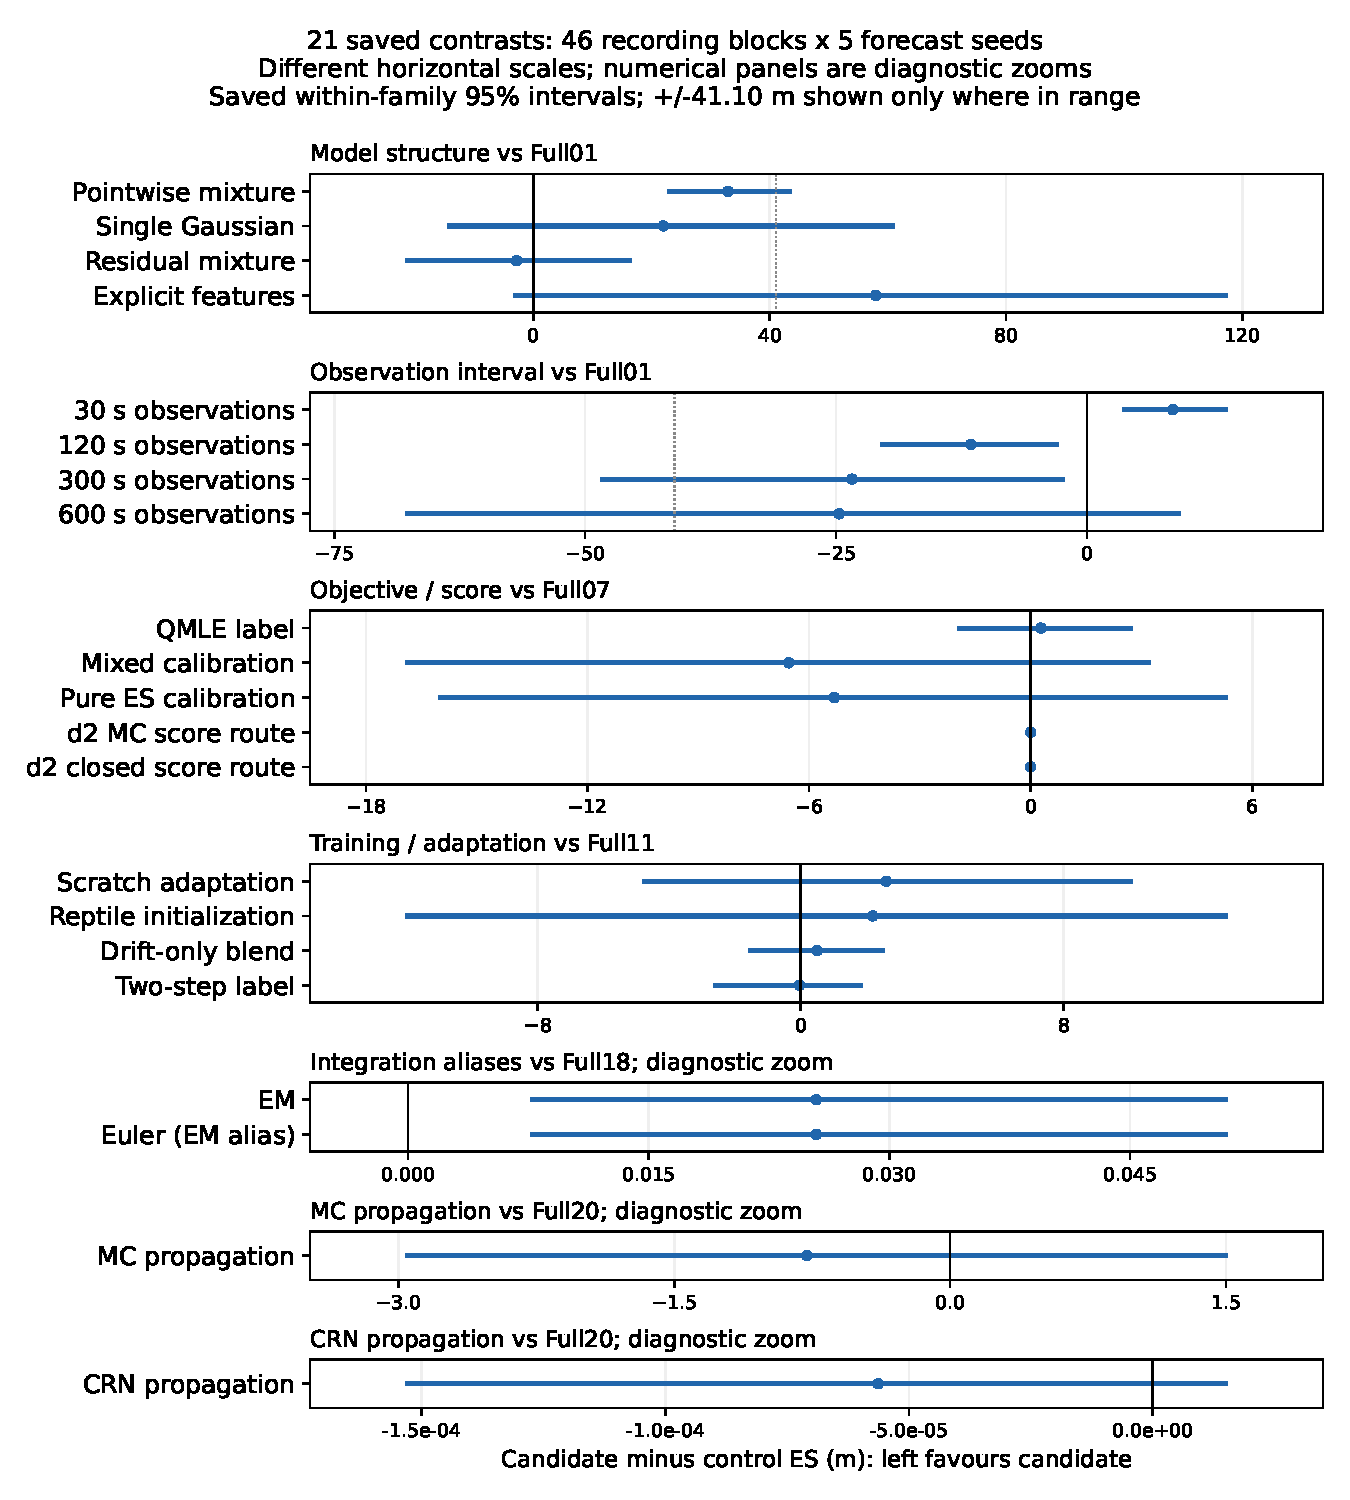
\includegraphics[height=.80\textheight,width=\linewidth,keepaspectratio]{../figures/preliminary-method-effects.pdf}
\caption{全部 21 个保存配对比较，各面板明确使用不同横轴尺度。
点是记录块平均的候选减对照 ES，线段是已保存的家族内同时 95\% 区间。
各面板写明 Full 对照，零左侧有利于候选。数值组单独放大用于诊断，不表示实际效果更大。
\(\pm41.10\) 米的实际意义虚线只在轴范围内绘制，小尺度面板的界在轴外；
放大或越过一条线本身均不构成资格裁定。
七个面板对应五个方法族：积分别名、MC 传播和 CRN 传播是数值族的三个诊断轴。
精细数值和别名仍见表~\ref{tab:preliminary-method-effects}。}
\label{fig:preliminary-method-effects}\hypertarget{fig:preliminary-method-effects}{}
\end{figure}
\begin{figure}[p]
\centering
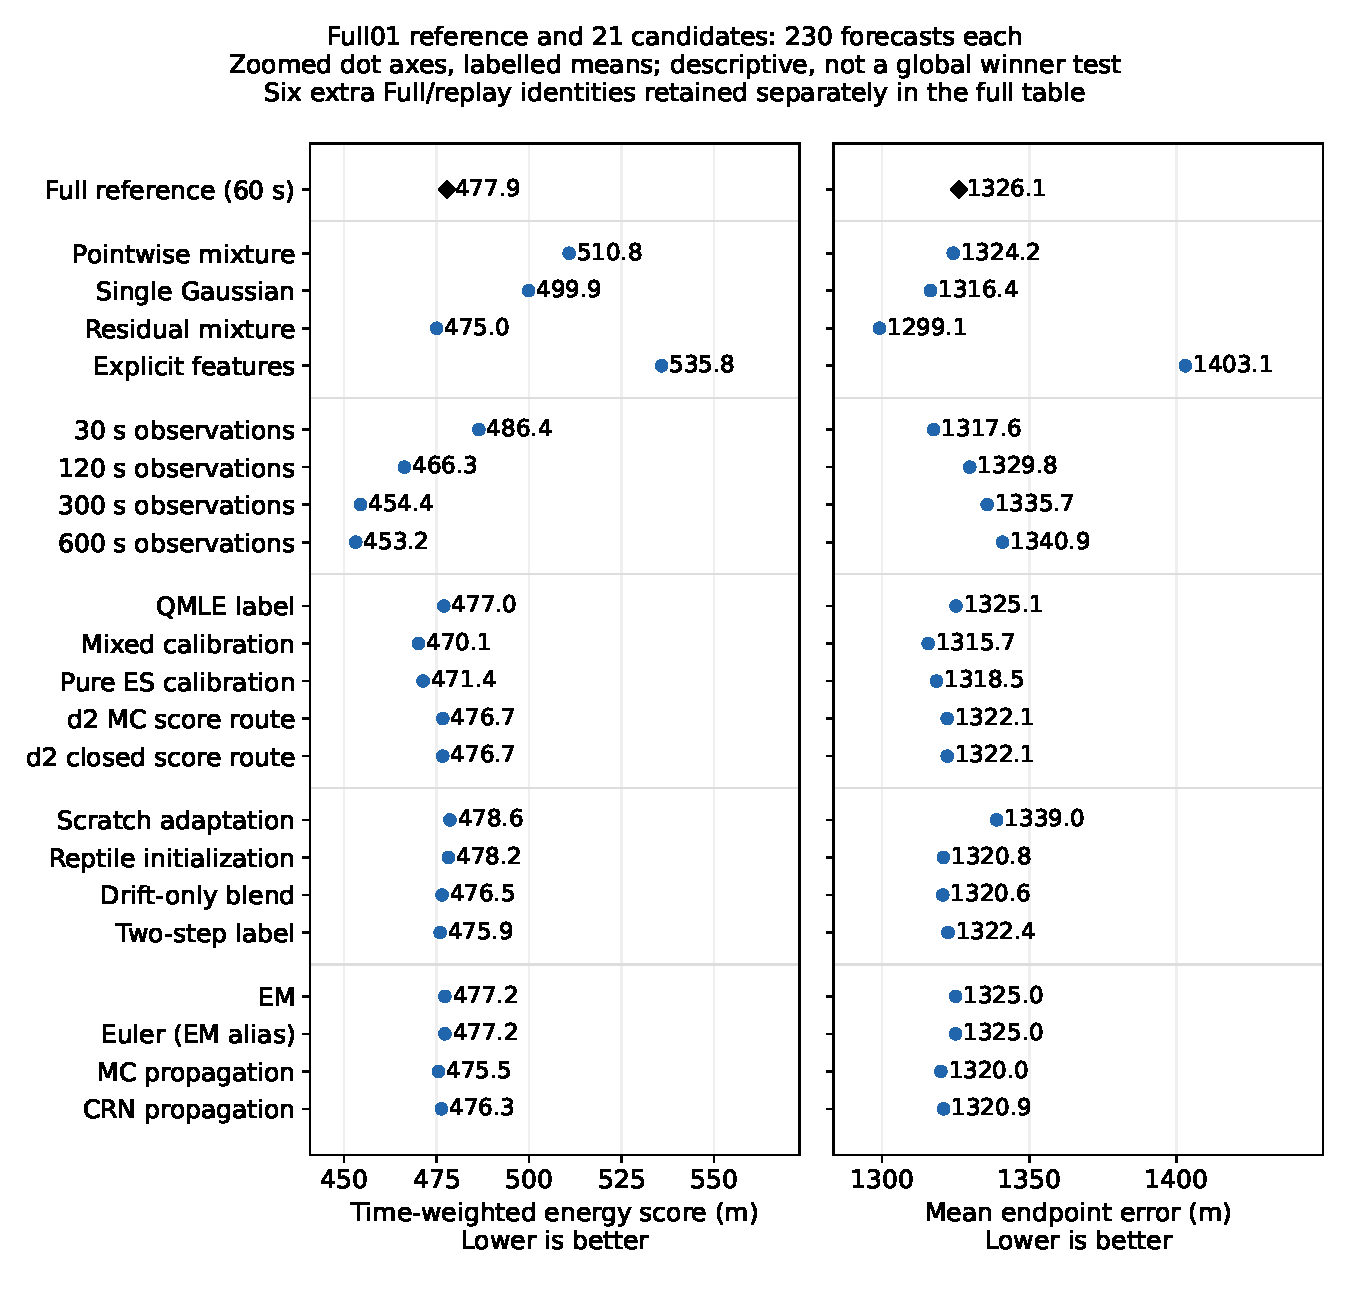
\includegraphics[height=.72\textheight,width=\linewidth,keepaspectratio]{../figures/preliminary-method-absolute.pdf}
\caption{Full01 参考与全部 21 个候选，以数值标注保存的绝对 ES 与终点误差均值，单位米。
两侧点图横轴均已放大，越低越好；点间距离不是配对效应估计。观测变体按间隔递增排列。
六个额外 Full／replay 角色仅在本图省略，仍分别保留于表~\ref{tab:all-method-absolute}，
不平均。每行完整使用 230 项预测；评分路线和别名不是独立算法。
这是描述图，不是全局最佳者检验。}
\label{fig:preliminary-method-absolute}\hypertarget{fig:preliminary-method-absolute}{}
\end{figure}

\FloatBarrier

\section{时域误差与经验覆盖率}
Full01 的加权 ES 为 477.85 米，而约 30 分钟平均终点误差为 1326.09 米，
两者不是同一个量。保存的全方法汇总逐时刻报告边际 ES，位置准确性则只保留
四目标平均 ADE 与末目标 FDE；这两个汇总不能确定前三个时刻的均值位置误差，
ES 也不能转换成它们，因此不据此重建完整位置误差曲线。
已有地图案例另保留四时刻均值误差，见第~\ref{sec:case-horizons}~节；
它们是地形示例，不能代替全方法准确性结果。
表~\ref{tab:preliminary-coverage} 展示边际 ES 随时域增大，
且较长时域的名义 90\% 预测圆经验覆盖率明显低于标称水平。
覆盖率是相同 46 个目标各自五个模拟集合的覆盖指示平均，
不能视为 230 个独立实际目标。这里仅报告描述性比例，
不增加新的覆盖率检验家族或置信区间，也不能唯一归因于漂移、扩散或混合机制。

\begin{table}[htbp]
\centering
\small
\caption{完整 Full01 主网格的阶段描述性评分；实际原始目标时间遵循登记容差。}
\label{tab:preliminary-coverage}\hypertarget{tab:preliminary-coverage}{}
\begin{tabular}{@{}rrr@{}}
\toprule
名义时域（分钟） & Full01 ES（米） & 90\% 预测圆覆盖率（\%）\\
\midrule
1 & 50.57 & 95.65\\
5 & 243.23 & 37.83\\
15 & 609.27 & 35.22\\
30 & 1008.35 & 46.52\\
\bottomrule
\end{tabular}
\end{table}

\paragraph{完整配置与时域的对应。}
图~\ref{fig:all-method-horizons} 将展示扩展到全部28个原方法主配置，
完整数值见表~\ref{tab:all-method-horizons}。
30分钟时域的保存边际ES均值介于941.89--1197.62米；全部名义90\%预测圆的
覆盖率均值都低于90\%，范围21.74\%--79.13\%。
这是跨配置范围，不是置信区间、人群界限或全局最佳模型检验。
加权主指标可能掩盖随时域变化的取舍：残差混合模型在5与15分钟的ES低于Full01
（228.87对243.23米；598.70对609.27米），30分钟却更高（1022.19对1008.35米）。
这里不新增逐时域显著性检验。边际ES是分布评分，不是预测均值位置误差；
覆盖率更高也不能脱离标称概率和区域大小解释为校准更好。
这些仍是原名义目标时域，不是新增插值的精确时间预测。
\hyperref[sec:target-times]{保存目标时钟描述}绑定三个已展示模型，
不是对全部28个配置预测数组的认证。另已完成的全保存输出审计覆盖完整评分网格；
该局部描述和全量审计均不认证目标时钟的物理来源。
\begin{figure}[p]
\centering
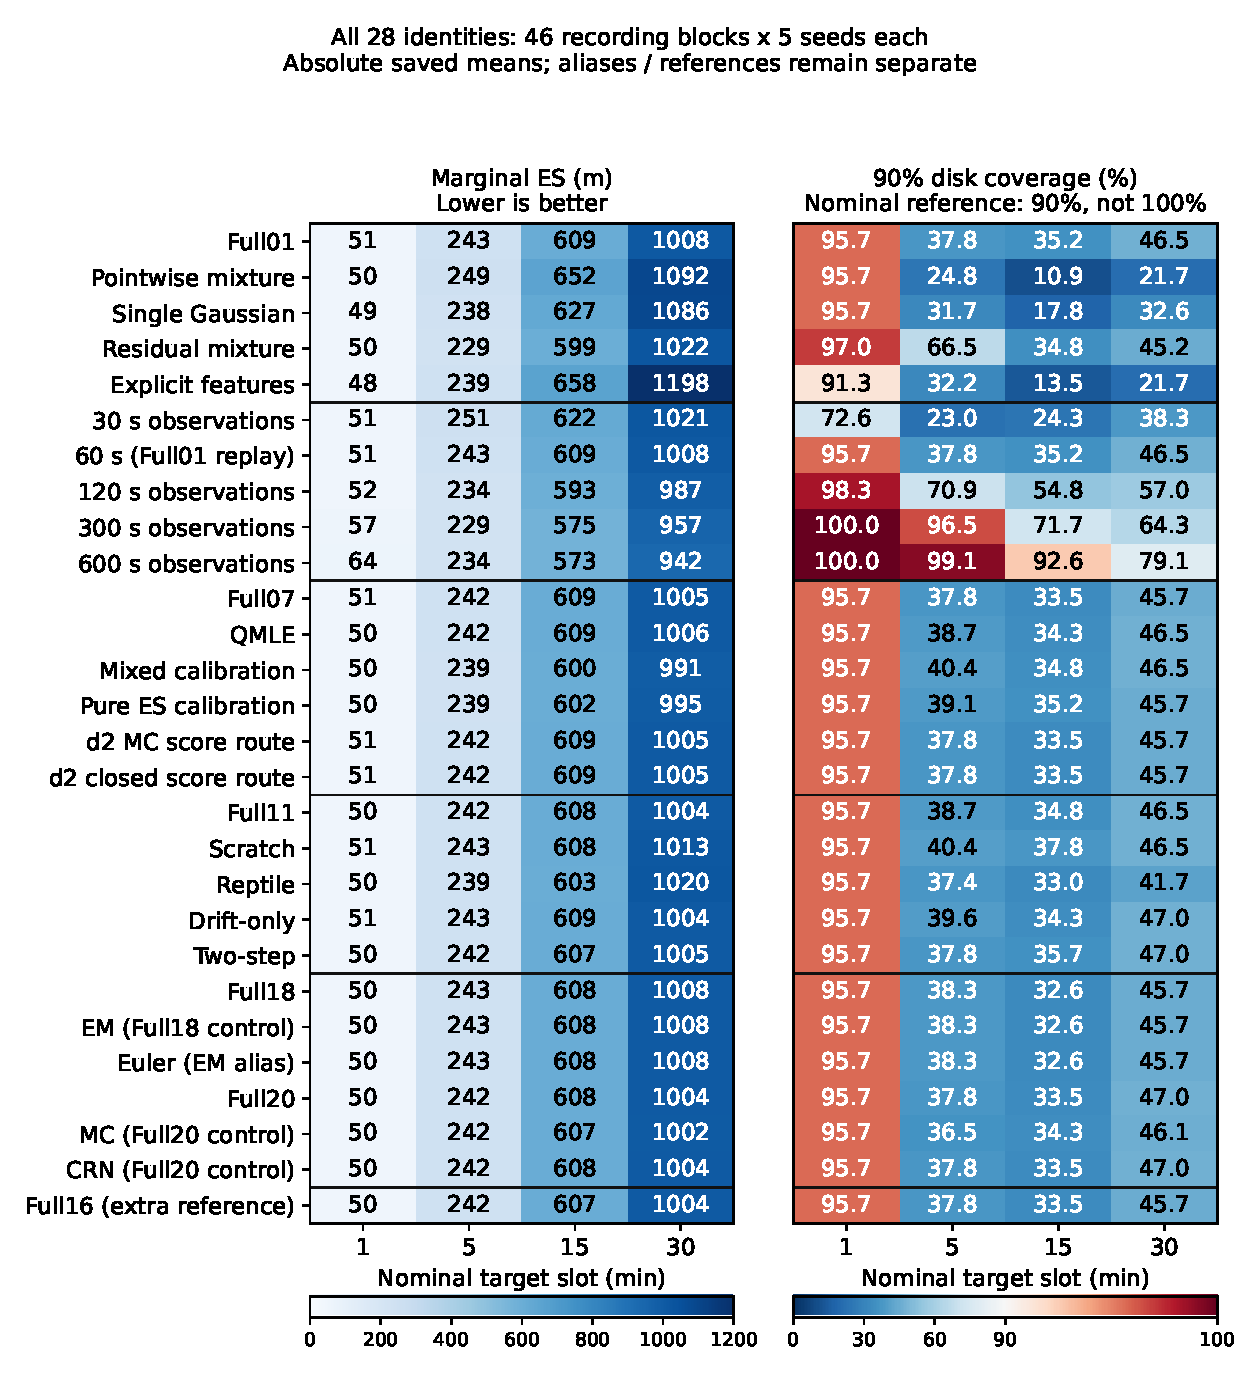
\includegraphics[height=.79\textheight,width=\linewidth,keepaspectratio]{../figures/revision46-corrections-v1/method-horizon-overview.pdf}
\caption{全部28个主组保存配置在四个名义目标时域的概览；没有新增中间时刻预测。左：边际ES（米），越低越好。右：名义90\%预测圆的实际覆盖率（\%）；校准参考是90\%而不是100\%，本图不显示区域大小。每格平均同一46块、五个种子。概览ES舍入到整数米，覆盖率保留一位小数；完整精度和全部角色保留于保存投影及表~\ref{tab:all-method-horizons}。行按登记家族而非性能排序；别名与不同Full对照不合并，舍入相似不证明等价。这是描述展示，不是新增逐时域检验或最终资格。}
\label{fig:all-method-horizons}
\end{figure}


\FloatBarrier
\paragraph{全部配置的区域大小与覆盖。}
图~\ref{fig:all-method-regions}与表~\ref{tab:all-method-regions}将联合区域描述
扩展到全部原方法主配置，仍使用相同6440份保存评分、46块和五个种子。
每个名义90\%预测圆格子同时给平均面积及目标包含率，表中另给平均半径。
平均的是各保存圆面积，而不是平均半径的平方；完整保存汇总保留四个概率水平、
四个目标时域。此次扩展只读取已有评分数字，不重评分粒子、不插值目标、不新增预测。

30分钟时，28配置的90\%圆平均面积为1.247--12.609平方公里，
实际覆盖率为21.74--79.13\%，均低于名义90\%。dt600在这份有限展示中面积最大、
观察覆盖率最高：12.609平方公里、79.13\%；Full01为4.534平方公里、46.52\%。
其面积约为Full01的2.78倍，平均终点误差却稍高（1340.94对1326.09米）。
因此覆盖率较高不能同时证明区域更集中、点预测更准及概率已校准。
dt600改变拟合观测间隔、历史输入和噪声估计，不只是预测积分步长；
这些描述比较不能识别哪一项改变导致了该模式。

面积—覆盖关系也不是跨时域一致的。5分钟时，残差混合的平均面积大于Full01
（0.400对0.294平方公里），覆盖率也更高（66.52\%对37.83\%）；
30分钟时，其面积更小（3.079对4.534平方公里），覆盖率略低（45.22\%对46.52\%）。
展示揭示的是随时域变化的描述性取舍，不是普遍的大小—质量规则、全局赢家检验或因果机制。
不新增逐时域区间或校准调整；逐块诊断仍是下文三个模型的描述。已完成的独立输出复算
不将这三个示例升级为全配置的逐块校准证据。
\begin{figure}[p]
\centering
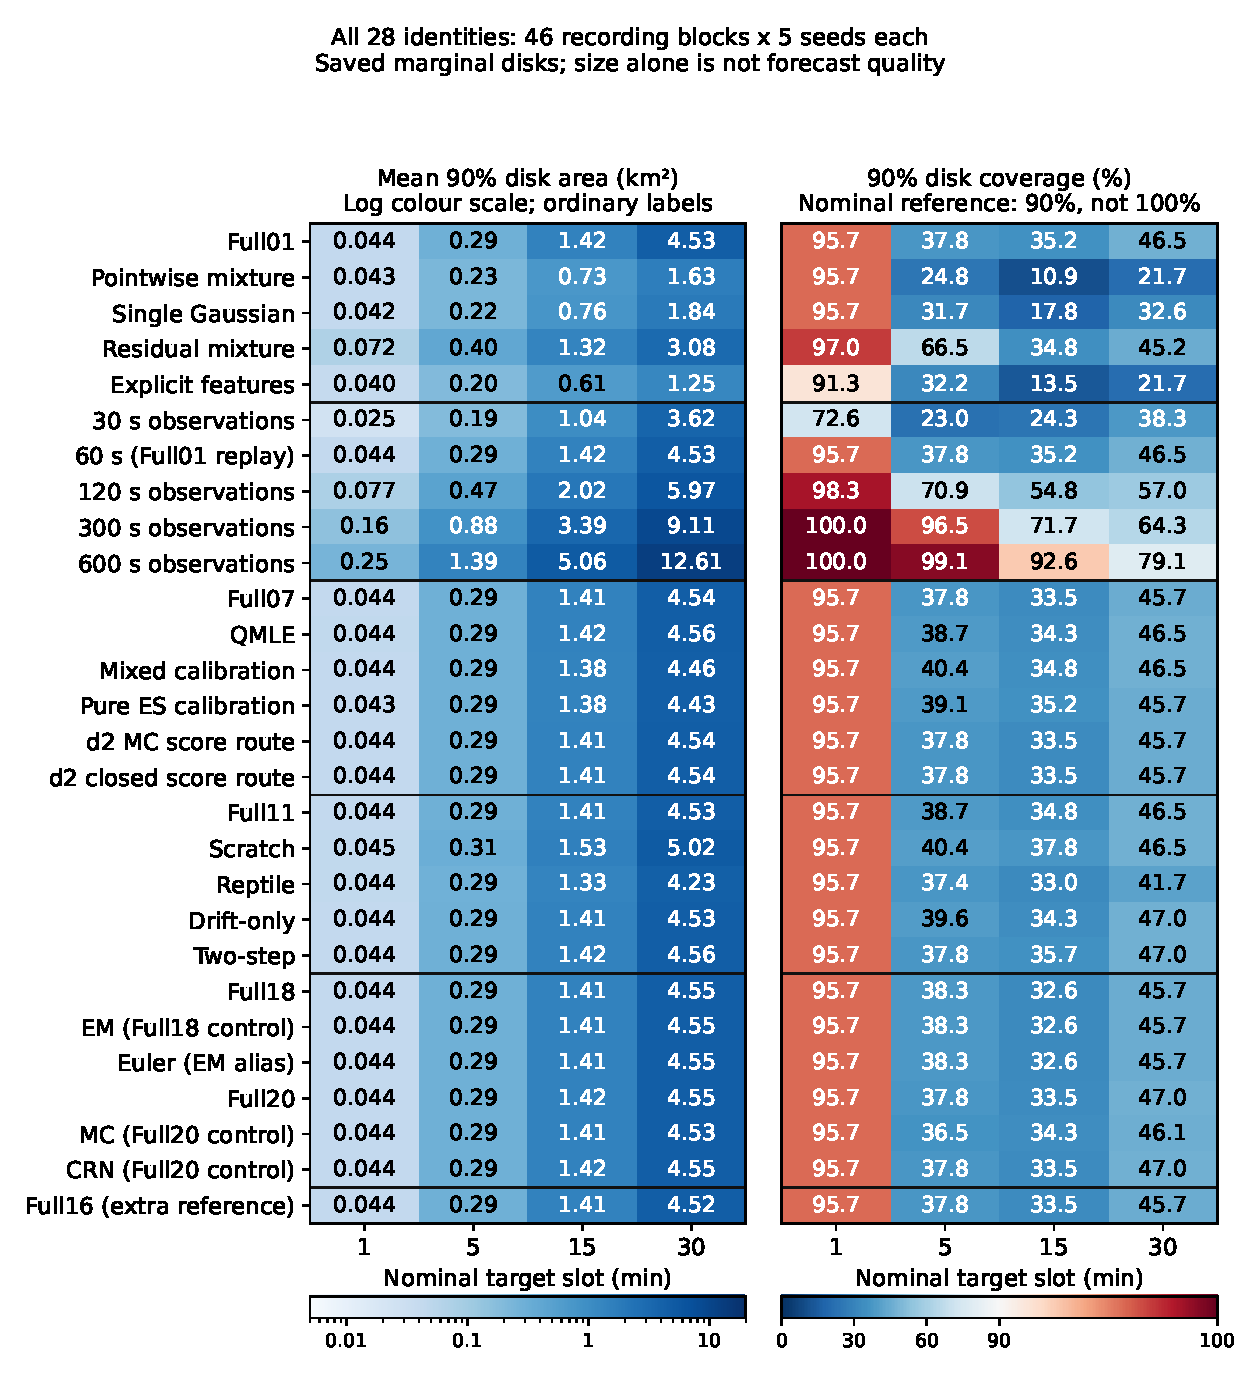
\includegraphics[height=.76\textheight,width=\linewidth,keepaspectratio]{../figures/revision46-corrections-v1/method-region-overview.pdf}
\caption{28配置在四个原目标时域的完整区域大小—覆盖展示。左：名义90\%预测圆平均面积（km$^2$）；颜色采用对数尺度，以同时显示短、长时域面积，格内标注仍为普通面积。右：实际目标包含率（\%），标称参考是90\%而不是100\%。面积和覆盖率都不能单独作为质量排名。行按登记方法家族而非观察性能排列，保留别名和各Full对照。每格先平均各块五个种子，再等权平均46块。仅为描述均值，没有新增检验、预测或重新校准；半径和精确值见表~\ref{tab:all-method-regions}及保存汇总。}
\label{fig:all-method-regions}
\end{figure}

\FloatBarrier

\paragraph{全部概率水平及扩大区域的代价。}
完整28配置的四档概率描述还显示，覆盖偏差不仅随时域改变，也随名义概率改变
（表~\ref{tab:all-level-coverage}）。1分钟时，24个配置的50\%圆覆盖率低于50\%，
但27个配置的90\%圆覆盖率高于90\%。因此，短时域单档覆盖较高不认证预测分布已经校准。
30分钟时，全部28配置在80\%、90\%、95\%三档均低于名义概率；
95\%实际覆盖范围为26.52--87.39\%。50\%档有27个低于名义值、一个恰好相等，
但单档相等不认证该配置其它概率水平。这里计数和范围针对保存的配置均值，
不是独立算法重复数或置信区间；冻结清单中的别名和Full对照仍保留。
表中同时给面积范围；扩大同一预测器的圆可以提高目标包含率，而不修复均值位置误差。
没有改变概率水平，也没有新增校准检验或拟合修正。

进一步描述此前已展示的 Full、GMM kernel、dt300 相同 690 项主要保存评分，
不新增预测、粒子重评分或推断检验。原评分均保存四个边际预测圆水平。
表~\ref{tab:full-calibration-area} 同时展示 Full 的覆盖与平均面积。
平均面积先在块内跨种子平均 \(\pi r_{p,t}^2\)，再等权平均 46 块，
不是 \(\pi\{\operatorname{mean}(r_{p,t})\}^2\)。

\begin{table}[htbp]
\centering\small
\caption{Full 完整主组的保存区域诊断。每格为实际覆盖率（\%）／平均圆面积（平方公里）；
列标题是名义概率，不是实际覆盖率。}
\label{tab:full-calibration-area}\hypertarget{tab:full-calibration-area}{}
\begin{tabular}{rrrrr}
\toprule
时域（分钟） & 50\% & 80\% & 90\% & 95\%\\
\midrule
1 & 33.04 / 0.013 & 87.39 / 0.031 & 95.65 / 0.044 & 96.52 / 0.057\\
5 & 6.52 / 0.094 & 25.65 / 0.210 & 37.83 / 0.294 & 50.43 / 0.378\\
15 & 9.57 / 0.539 & 24.35 / 1.062 & 35.22 / 1.415 & 43.91 / 1.753\\
30 & 33.48 / 2.002 & 37.39 / 3.552 & 46.52 / 4.534 & 52.17 / 5.496\\
\bottomrule
\end{tabular}
\end{table}

长时域的不匹配不止出现在 90\% 水平：30 分钟时 Full 的名义 95\% 预测圆，
跨模拟集合平均仅覆盖 52.17\% 的目标。1 分钟时，名义 50\% 和 90\% 的覆盖率
分别为 33.04\% 与 95.65\%，说明不匹配也随概率水平变化。
这些是描述性测量，不是新显著性声明，也未证明某个具体故障机制。

\begin{table}[htbp]
\centering\small
\caption{相同原 46 块、每模型五个模拟集合的 30 分钟名义 90\% 预测圆。
没有足够覆盖时面积较小不一定更好；覆盖较大也不必然意味着校准更好。}
\label{tab:model-region-size}\hypertarget{tab:model-region-size}{}
\begin{tabular}{lrrr}
\toprule
模型 & 覆盖率（\%） & 平均面积（平方公里） & 平均半径（米）\\
\midrule
Full & 46.52 & 4.534 & 1183.6\\
GMM kernel & 45.22 & 3.079 & 989.5\\
dt300 & 64.35 & 9.109 & 1692.8\\
\bottomrule
\end{tabular}
\end{table}

dt300 的 30 分钟覆盖率高于 Full，但平均圆面积约为后者两倍，覆盖仍远低于名义 90\%。
其终点均值误差也略高（1335.73 对 1326.09 米）。因此 ES 改善或覆盖增加，
不能解释为同时获得更紧、更准确且已校准的预测。GMM 的 30 分钟圆较小也不证明精度更好。

这三模型是此前已选示例的事后描述，
不是全模型排行、新检验家族或模型选择规则。
投影 \path{paper/pirc17/calibration-description-v1.json} 保留完整原 690 项评分绑定，
不包含私有轨迹标识或坐标。其 ES、FDE 与 90\% 覆盖率均核对到未改动的原阶段表。
缺失、失败、重复或来源不符会使整个投影失败。独立保存输出审计已另行完成；
本描述性投影本身不建立校准或参与者独立性。

\begin{figure}[htbp]
\centering
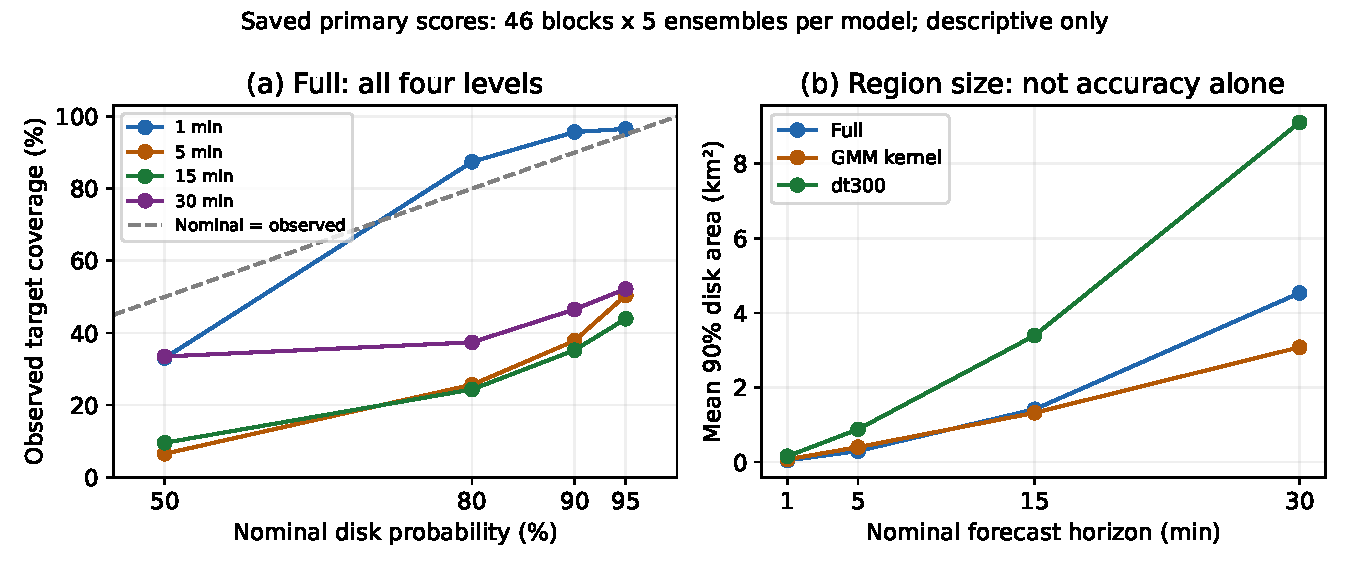
\includegraphics[width=\linewidth]{../figures/preliminary-calibration-area.pdf}
\caption{已保存的校准与区域大小诊断，不是新增实验。左：Full 各时域的实际覆盖对名义概率，
对角虚线表示名义一致。右：此前三个模型的 90\% 预测圆平均面积。
连线仅在四个已测水平或时域间引导视线，没有评价中间目标、整路径联合覆盖或新增统计检验。}
\label{fig:calibration-area}\hypertarget{fig:calibration-area}{}
\end{figure}

\paragraph{记录块之间的差异。}\label{sec:block-calibration}\hypertarget{sec:block-calibration}{}
对固定模型、目标时刻和预测圆概率水平，先在原 46 个记录块内平均五个预测种子：
\begin{equation}
 C_b=\frac{1}{5}\sum_s\mathbf{1}\{y_b\in D_{bs}\},\qquad
 a_b=\frac{1}{5}\sum_s\frac{|D_{bs}|}{10^6}.
 \label{eq:block-calibration-summary}\hypertarget{eq:block-calibration-summary}{}
\end{equation}
\(D_{bs}\) 是已保存的边际预测圆，\(C_b\) 是描述性覆盖比例，\(a_b\) 是以平方公里表示的平均面积。
五个种子重复预测同一个真实目标，并非五个独立观测。单块 \(C_b\) 只能取 0.2 的倍数。
表~\ref{tab:block-calibration} 给出记录块间中位数与四分位范围，
按 \((46-1)p\) 线性插值的分位数不必落在该网格上，也不是置信区间。
\path{paper/pirc17/calibration-block-description-v1.json} 保留全部四档原概率水平和四个时域；
本表和图~\ref{fig:block-calibration} 仅展示名义 90\% 预测圆。

\begin{table}[htbp]
\centering\small
\caption{原 46 块的名义 90\% 预测圆分布。
覆盖和面积为中位数 [第25、75百分位]；末两列是五个种子均未覆盖／均覆盖目标的块数。}
\label{tab:block-calibration}\hypertarget{tab:block-calibration}{}
\begin{tabular}{@{}lrl lrr@{}}
\toprule
模型 & 分钟 & 覆盖（\%） & 面积（平方公里） & 0/5 & 5/5\\
\midrule
Full & 1 & 100 [100, 100] & 0.043 [0.042, 0.046] & 2 & 44\\
Full & 5 & 0 [0, 100] & 0.280 [0.261, 0.308] & 26 & 16\\
Full & 15 & 0 [0, 100] & 1.285 [1.150, 1.557] & 29 & 15\\
Full & 30 & 10 [0, 100] & 4.022 [3.405, 4.966] & 23 & 20\\
\midrule
GMM kernel & 1 & 100 [100, 100] & 0.072 [0.070, 0.074] & 1 & 44\\
GMM kernel & 5 & 100 [5, 100] & 0.401 [0.389, 0.411] & 12 & 28\\
GMM kernel & 15 & 0 [0, 100] & 1.322 [1.300, 1.357] & 28 & 14\\
GMM kernel & 30 & 0 [0, 100] & 3.088 [3.000, 3.179] & 24 & 20\\
\midrule
dt300 & 1 & 100 [100, 100] & 0.155 [0.150, 0.159] & 0 & 46\\
dt300 & 5 & 100 [100, 100] & 0.871 [0.832, 0.894] & 1 & 44\\
dt300 & 15 & 100 [20, 100] & 3.264 [3.060, 3.497] & 11 & 31\\
dt300 & 30 & 100 [0, 100] & 8.518 [7.707, 9.564] & 16 & 29\\
\bottomrule
\end{tabular}
\end{table}

30 分钟时，Full 有 23/46 块五个种子均未覆盖，20 块均覆盖，尽管总体覆盖率为 46.52\%。
其面积中位数为 4.022 平方公里 [3.405, 4.966]，范围 2.963--11.551 平方公里。
dt300 的覆盖比例中位数为 100\%，仍有 16 块五个种子均未覆盖；
面积中位数为 8.518 平方公里 [7.707, 9.564]。
总体平均或较高中位数都不能证明条件校准可靠、可部署，或确定具体哪个组件导致未覆盖。

不暴露坐标的例子是匿名块 B13：在原排序中，它是首个 30 分钟 Full 为 0/5、dt300 为 5/5 的块。
Full、GMM、dt300 分别为 0/5、0/5、5/5 覆盖，平均面积分别为 3.489、3.204、8.260 平方公里。
该例是在看过结果后选择，仅解释区域大小与覆盖，不用于优越性推断。
不公开路线或地理身份；真实地图案例的独立发表许可仍未核实。

\begin{figure}[p]
\centering
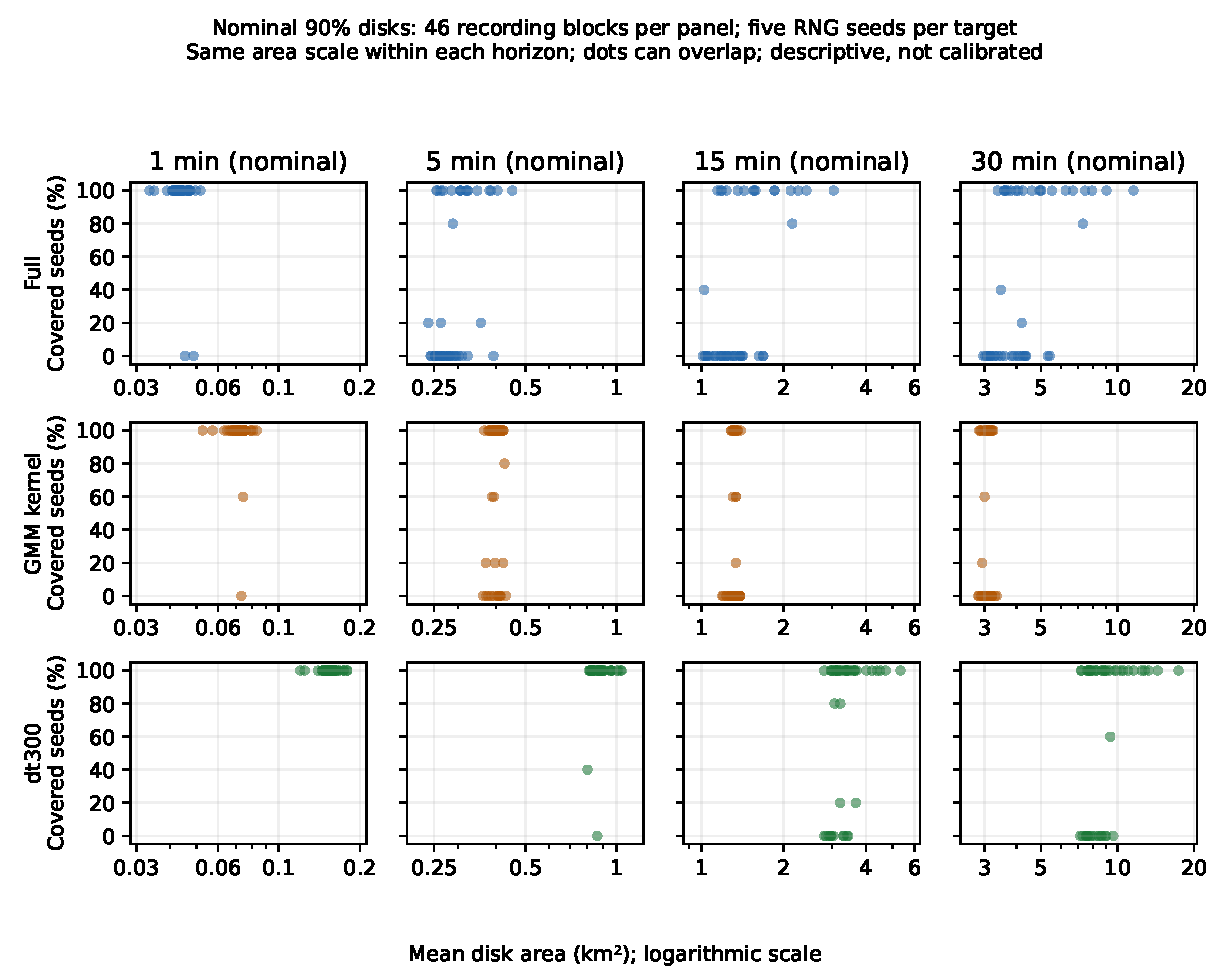
\includegraphics[width=\linewidth]{../figures/preliminary-calibration-blocks.pdf}
\caption{此前三个模型在四个名义时域的配对记录块面积与覆盖。
每个点是同一块五个预测种子的平均，点可能重叠；横轴为对数面积，
同一时域各模型共用尺度。纵轴是五个保存预测圆覆盖同一目标的比例，
不是 46 个总体校准估计。没有整路径联合覆盖、新假设检验或事后半径重缩放。}
\label{fig:block-calibration}\hypertarget{fig:block-calibration}{}
\end{figure}

已知速度模式的结构及观测间隔家族各含一行必需失败，整个家族保持不可用。
其他完整的六块次要汇总只作描述。缺评分不填零，不删除失败行形成有利成功交集，
也不以主要模式数据替换失败的次要模式。

\begin{figure}[htbp]
\centering
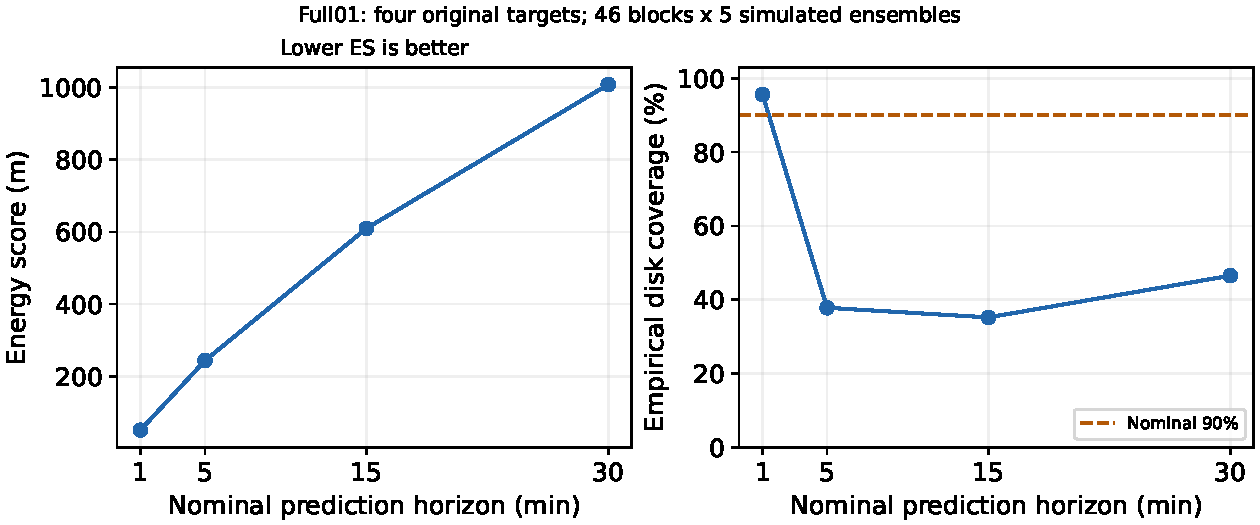
\includegraphics[width=\linewidth]{../figures/revision46-corrections-v1/preliminary-full-horizons.pdf}
\caption{Full01 四个原目标的真实已保存汇总评分与覆盖率。虚线是名义 90\%；
实际 30 分钟覆盖率仅 46.52\%。连线只引导视线，不代表中间观测或生存曲线。
这是分布级汇总，不是轨迹／地图叠图，也不是 230 个独立目标的测量。}
\label{fig:preliminary-full-horizons}\hypertarget{fig:preliminary-full-horizons}{}
\end{figure}


\section{按起点覆盖类别的描述性方法结果}
\label{sec:origin-cover-results}\hypertarget{sec:origin-cover-results}{}
为说明环境覆盖，表~\ref{tab:origin-cover-methods} 使用 Full、GMM、dt300 原 $3\times46\times5$ 主组的完整 690 项保存评分。
每个记录块先平均五个模拟种子，再在原 WorldCover 起点类别内等权平均记录块。
ES 仍为四个登记目标时刻的平均，FDE 为最后目标误差；按类别块数加权后与原方法主表一致。
缺失、失败、重复或来源不符的任何项会使整个描述性投影失败，不使用成功交集替代。

\begin{table}[htbp]
\centering\small
\caption{起点类别的描述性均值，数值为 ES/FDE（m）；不提供分组置信区间、假设检验或环境效应裁定。}
\label{tab:origin-cover-methods}\hypertarget{tab:origin-cover-methods}{}
\begin{tabular}{lrrrr}
\toprule
起点像素 & 记录块 & Full & GMM & dt300\\
\midrule
树木 & 27 & 427.66/1184.64 & 420.85/1153.52 & 414.59/1203.95\\
草地 & 9 & 556.86/1597.16 & 557.16/1587.72 & 514.09/1579.13\\
耕地 & 3 & 623.14/1678.49 & 589.40/1591.57 & 600.89/1775.32\\
建筑用地 & 7 & 507.60/1372.16 & 529.38/1364.23 & 468.75/1342.70\\
\bottomrule
\end{tabular}
\end{table}

这些是已看结果后的描述，不是预登记分组推断。例如树木和耕地起点组中，dt300 的平均 ES 较低而 FDE 较高；
建筑用地组中 GMM 的 ES 较高而 FDE 略低。这示范指标排序的区别，不是因果地形效应或稳定的分环境模型优越性。
耕地组仅三个记录块，不是 15 条独立轨迹。另七个未覆盖的起点类别在投影中保留 null 指标。
正式方法推断仍使用全部 46 块；实际地形效应仍须依照独立登记的地形比较及其证据资格判定。

\FloatBarrier
\subsection{已完成的恒速惯性参考}
\label{sec:inertial-primary}
登记的惯性参考使用保存的因果初始速度外推：$\widehat x^{\mathrm{I}}(t)=x_0+t\widehat v_0$。它是一条确定性路径，不是新拟合的 SDE，也不是五次重复的粒子预测。原58条参考路径均已有保存评分；表~\ref{tab:inertial-primary}、\ref{tab:inertial-horizons} 使用事前规定的完整46块主人群，不包含12个次要起点。每条参考与 Full 的起点、目标身份和实际目标时刻一致。先在每块内平均 Full 的五个预测种子，再等权平均46个记录哈希块；不把一条参考重复计成五份样本。

\begin{table}[htbp]\centering\small
\caption{相同主起点和保存目标时刻。全部误差单位为米，越低越好。ES 评价预测分布，ADE/FDE 评价均值路径；惯性参考是点质量分布，故其 ES 等于位移误差。份数指保存预测，不是独立人员或拟合模型数。仅描述均值，没有新增置信区间、显著性检验或资格结论。}\label{tab:inertial-primary}
\begin{tabular}{@{}lrrrrr@{}}\toprule
模型 & 预测份数 & 块数 & 加权 ES & ADE & FDE\\\midrule
惯性参考 & 46 & 46 & 824.73 & 824.73 & 2095.78\\
Full & 230 & 46 & 477.85 & 636.11 & 1326.09\\
\bottomrule\end{tabular}\end{table}

\begin{table}[htbp]\centering\small
\caption{四个名义时域的平均边际 ES，单位米，越低越好。按未改变的原30秒容差，保存时钟上的实际目标分别为49--67、294--305、889--910、1785--1814秒；没有插值目标或新增模拟。}\label{tab:inertial-horizons}
\begin{tabular}{@{}lrrrr@{}}\toprule
模型 & 1 分钟 & 5 分钟 & 15 分钟 & 30 分钟\\\midrule
惯性参考 & 31.17 & 237.93 & 934.03 & 2095.78\\
Full & 50.57 & 243.23 & 609.27 & 1008.35\\
\bottomrule\end{tabular}\end{table}

Full 减惯性参考的均值差为：加权 ES -346.87 米、ADE -188.62 米、FDE -769.69 米。46块中有34块的 Full 加权 ES 严格更低。但1、5分钟的惯性平均 ES 更低，15、30分钟的 Full 更低，因此汇总收益并非所有时域都一致。

这是对既有评分的事后描述，不是登记的组件对比或独立核验后的优越性结论。不从34/46计数作统计推断，记录哈希也不认证独立参与者。原验证数据确定的 $\delta=41.100259$ 米不按此次最终评估惯性均值重新设定。原输出核验、最终卡片与人工审阅仍待完成；不能据此声称优于引用的外部模型或已满足部署校准。
\FloatBarrier

\FloatBarrier
\subsection{每个保存目标时刻的位置误差}
\label{sec:point-error-horizons}
ES 评价整个预测分布，不是分布均值到真实位置的距离。表~\ref{tab:point-error-horizons} 将此前 Full/GMM/dt300 对照与惯性参考的这个距离单独列出，不构成全部28配置的新排行。使用原保存评分圆盘的中心 $c_{m,b,s,k}$（512粒子的均值，或确定性参考位置）和同一原目标 $y_{b,k}$，两者均在原起点局部评分坐标系中。不需打开预测数组、重新计算粒子评分、插值目标或模拟。

对模型 $m$，先在每个记录哈希块内平均其 $S_m$ 个原预测种子的误差，再等权平均全部46块。三个概率配置的 $S_m=5$，惯性参考的 $S_m=1$，不将一条参考计成五份：
\begin{equation}
\bar e_{m,k}=\frac{1}{46}\sum_{b=1}^{46}
\frac{1}{S_m}\sum_{s=1}^{S_m}\lVert c_{m,b,s,k}-y_{b,k}\rVert_2.
\label{eq:point-error-horizon-mean}
\end{equation}

\begin{table}[htbp]\centering\small
\caption{原保存均值位置的平均位移误差，单位米，越低越好。四列是原名义1/5/15/30分钟目标；保存时钟实际范围49--67、294--305、889--910、1785--1814秒，原30秒容差不变。份数是保存预测，不是独立目标或人员。仅描述数值，不做分时域推断。}\label{tab:point-error-horizons}
\begin{tabular}{@{}lrrrrr@{}}\toprule
模型 & 份数 & 1 分钟 & 5 分钟 & 15 分钟 & 30 分钟\\\midrule
Full & 230 & 73.77 & 332.31 & 812.26 & 1326.09\\
GMM & 230 & 71.92 & 323.79 & 792.99 & 1299.11\\
dt300 & 230 & 75.88 & 340.10 & 825.76 & 1335.73\\
惯性参考 & 46 & 31.17 & 237.93 & 934.03 & 2095.78\\
\bottomrule\end{tabular}\end{table}

全部736份所选保存结果对应同一184个目标位置。逐份检查四时刻误差的算术均值及最后一项，在浮点舍入精度内分别复现原保存 ADE 和 FDE，最大差异小于 $10^{-12}$ 米。先跨种子平均位置再取欧氏距离会得到另一估计量，本表未这样处理。

惯性参考在1、5分钟的平均点误差更低，Full 在15、30分钟更低。GMM 在四时域的描述性均值均略低于 Full；相反，dt300 虽有更低的原汇总 ES，四时域均值位置误差却均大于 Full。因此，分布评分改善不自动等于均值路径位置改善。dt300 指训练观测间隔，不是积分步长。事后均值不证明统计优越性、独立人员泛化或部署精度；原最终推断、输出核验及审阅仍待完成。
\FloatBarrier



\section{边缘CRPS与单次预测内粒子终点误差分位数}
\label{sec:secondary-score-diagnostics}\hypertarget{sec:secondary-score-diagnostics}{}
表~\ref{tab:crps-endpoint-diagnostics}沿用上面已比较的四个模型，不按新诊断指标挑选表现最好的模型。
坐标CRPS以米评价局部东／北边缘分布，各自在其坐标上越小越好；两个边缘较好并不认证
联合分布、依赖结构或预测圆校准。不把两个坐标分数相加后称为联合ES。

下半表区分均值位置FDE与粒子终点误差分位数。每次原预测保存的$q_{.50}$、$q_{.90}$、
$q_{.95}$，是该预测的粒子到该例实际终点的距离分位数；随后对这些已保存分位数
按种子与记录块求均值。它们不是跨案例FDE总体分位数，不是合并不同案例粒子后的
分位数，也不是以预测均值为中心的圆半径。不选择最优粒子。惯性参考只有一个点，
所以每次预测内三个分位数在汇总前就都等于该次FDE。

这些诊断说明一项评分不能代替全部预测质量。名义30分钟时，dt300的东／北CRPS低于Full01
（687.11/524.07对737.72/535.72米），但均值位置FDE略高（1335.73对1326.09米），
预测内$q_{.95}$的均值也更大（2827.57对2346.62米）。GMM对应的$q_{.95}$为2138.12米，
不是承诺半径2138.12米的预测圆具有95\%目标覆盖率。这些均值仅作描述，
不新增逐时域显著性、普遍优势或因果解释，前述长时域欠覆盖仍是性能局限。

完整\path{paper/pirc17/secondary-scores-v1/}补充材料保留原11368行评分的全部120个配置／模式
视图及480个重复时间视图，包括五个含必需失败、均值为null的配置／模式视图。
先在起点内平均种子，再对相同记录哈希块等权平均；惯性路径不复制五次。
不重复预测、粒子评分或重采样。匿名投影绑定原导出\texttt{29cb892f}、审计\texttt{8ff917ad}、
分析\texttt{d1d67a3b}；保留实际记录目标时刻范围，不认证物理UTC或参与者独立性。
\begin{table}[htbp]
\centering\small
\caption{保存的边缘CRPS及单次预测内粒子终点误差分位数，单位米。CRPS在其坐标上越小越好，两个边缘不确定联合校准。随机配置各使用46个记录哈希块、五种子，共230次预测；惯性参考在相同46块上各有一条确定性路径。分位项是每次预测内粒子误差分位数的块／种子均值，不是总体FDE分位数、合并粒子分位数或最优粒子路径。保留原实际记录时刻，不新增逐时域假设检验。}
\label{tab:crps-endpoint-diagnostics}
\begin{tabular}{@{}lrrr@{}}
\toprule
模型 & 名义分钟 & 东坐标CRPS & 北坐标CRPS\\
\midrule
Full01 & 1 & 32.71 & 31.55\\
Full01 & 5 & 157.30 & 153.31\\
Full01 & 15 & 390.26 & 373.30\\
Full01 & 30 & 737.72 & 535.72\\
GMM & 1 & 32.58 & 31.51\\
GMM & 5 & 149.27 & 142.28\\
GMM & 15 & 384.50 & 367.09\\
GMM & 30 & 736.79 & 549.33\\
dt300 & 1 & 37.20 & 34.78\\
dt300 & 5 & 147.70 & 144.49\\
dt300 & 15 & 368.85 & 354.71\\
dt300 & 30 & 687.11 & 524.07\\
Inertial & 1 & 21.37 & 18.50\\
Inertial & 5 & 137.90 & 160.72\\
Inertial & 15 & 561.23 & 618.27\\
Inertial & 30 & 1297.37 & 1356.32\\
\bottomrule
\end{tabular}
\par\medskip
\begin{tabular}{@{}lrrrr@{}}
\toprule
模型 & 平均FDE & 均值$q_{.50}$ & 均值$q_{.90}$ & 均值$q_{.95}$\\
\midrule
Full01 & 1326.09 & 1564.98 & 2205.44 & 2346.62\\
GMM & 1299.11 & 1419.34 & 1979.14 & 2138.12\\
dt300 & 1335.73 & 1663.28 & 2585.48 & 2827.57\\
Inertial & 2095.78 & 2095.78 & 2095.78 & 2095.78\\
\bottomrule
\end{tabular}
\end{table}



\section{公开审查版暂不包含本地路线案例}
\label{sec:case-horizons}\hypertarget{sec:case-horizons}{}
完整本地工作稿保留三个真实地图案例及名义1、5、15、30分钟的位置分布。
本公开审查投影暂不包含路线地图和案例级诊断，等待轨迹隐私和地图公开权限核实。
不以合成数据替代缺图，也不新增预测。完整本地稿是单独的审查材料；
本投影不核验被保留在本地的证据，也不证明总体地形效应。

\clearpage

\section{保存人群描述的构造方法}
\label{sec:population-description-construction}\hypertarget{sec:population-description-construction}{}
时长、速率与来源标签表描述原候选总体，不构成新的资格筛选。
这里集中保留统计构造记录，使正文聚焦受限评估人群及其科学解释边界。

\paragraph{原窗口与入选起点的后续观测时长。}\label{sec:final-cohort-durations}\hypertarget{sec:final-cohort-durations}{}
表~\ref{tab:final-cohort-durations} 描述同一完整候选总体，而不是仅统计已成功的预测。
每个原窗口的后续时长定义为 $D=t_{\mathrm{last}}-t_{\mathrm{origin}}$。
全部 12,370 个窗口均保留原资格与选择，不裁剪或删除无效时间窗口。
窗口等权描述没有把同一记录的多个窗口当作多个独立主体。

\begin{table}[htbp]
\centering\small
\caption{保存时钟下，从原起点到最后观测的后续时长（秒）。总体行是分母，后四行互斥分割全部窗口；括号为四分位区间，不是置信区间。每个原窗口只计一次。}
\label{tab:final-cohort-durations}\hypertarget{tab:final-cohort-durations}{}
\begin{tabular}{@{}lrrrr@{}}
\toprule
窗口组 & 数量 & 中位数 [Q25,Q75] & 最小--最大 & $\geq1800$s\\
\midrule
已发布总体 & 12,370 & 69.8 [30,203] & 2--4183 & 130\\
时间条件排除 & 12,243 & 68 [29,194] & 2--2790 & 3\\
时间合格后地图排除 & 21 & 2311 [2108,2559] & 1800--3984 & 21\\
合格但未选中 & 60 & 2200 [1947,2570.2] & 1816--4183 & 60\\
选中主要起点 & 46 & 2323 [2034,2519] & 1808--4143 & 46\\
\bottomrule
\end{tabular}
\end{table}

已发布窗口的中位后续支持只有 69.8s，选中起点为 2,323s（约38.7分钟）。
全部候选中仅 130/12,370（约1.05\%）具有至少 1,800s 后续记录；
原时间资格只通过 127 项，因此“足够长”不是全部时间条件：
另三个长窗口仍在原时间排除组，本统计不据此修复或重定其原因。
地图有效性又排除 21 项，最后按已冻结选择规则取 46 个起点。
这说明当前名义30分钟任务条件于少量长且地图支持完整的轨迹，
不是一般短轨迹的部署性能，也没有用事后性能选择或改变预测时域。

这里的时长是保存时钟的相对差，不认证原物理UTC或真实采集历时。
更长的后续记录不表示模拟也延长：预测仍在原四个目标时刻取位置分布；
超过1,800s的实际末目标另见表~\ref{tab:actual-target-times}。
描述文件中的历史窗口支持也不等于实际保留的最后两/三个点割线缓冲。
保存速率另见下文；统计构造细节及完整各阶段汇总见
附录~\ref{sec:population-description-construction}。

\paragraph{原窗口与入选起点的保存速率。}\label{sec:final-cohort-speeds}\hypertarget{sec:final-cohort-speeds}{}
这里统计源表已保存的区间速率标量，不从发布位置或记录时钟重算速度。
对原窗口 $w$ 定义
\begin{equation}
 s_w=\operatorname{median}_{j=0,\ldots,n_w-1}s_{w,j},
 \label{eq:cohort-window-speed}\hypertarget{eq:cohort-window-speed}{}
\end{equation}
其中 $n_w$ 包含完整已发布观测窗口的全部点，也包含后续观测。
表~\ref{tab:final-cohort-speeds} 再对 $s_w$ 作窗口等权、线性分位数描述，
不是所有点混合计权或按历时加权的速率分布；同一记录的多个窗口不等于多个独立主体。

\begin{table}[htbp]
\centering\small
\caption{原窗口保存区间速率的窗口内中位数，再作窗口间描述（单位按保留构建脚本为m/s）。括号为四分位区间，不是置信区间。后四行互斥分割原总体；失败列指本描述统计失败，不是预测失败。}
\label{tab:final-cohort-speeds}\hypertarget{tab:final-cohort-speeds}{}
\begin{tabular}{@{}lrrrr@{}}
\toprule
窗口组 & 数量 & 中位数 [Q25,Q75] & 最小--最大 & 失败\\
\midrule
已发布总体 & 12,370 & 1.621 [1.191,1.949] & 0.097--4.067 & 0\\
时间条件排除 & 12,243 & 1.626 [1.191,1.954] & 0.097--4.067 & 0\\
时间合格后地图排除 & 21 & 1.192 [0.999,1.269] & 0.263--1.596 & 0\\
合格但未选中 & 60 & 1.460 [1.268,1.651] & 0.569--2.436 & 0\\
选中主要起点 & 46 & 1.486 [1.245,1.636] & 0.831--2.554 & 0\\
\bottomrule
\end{tabular}
\end{table}

源标量的末点填充及其与速度分量模长的区别见
附录~\href{audit-notes.pdf\#sec:source-reconciliation-details}{审查记录}；不移除窗口，
也不以成功子集替代任何失败组的分布。

已发布与最终入选的窗口间中位数分别为1.621与1.486 m/s。
与时长、地域描述合起来，它说明当前评估人群的构成，
不是显著性检验、物理速度校准，也不证明速度造成了任何预测差异。
未来观测只用于这项事后描述，不输入预测器或重定资格。
当前保留构建脚本与全量构建入口分别固定身份，但不在原发布认证绑定中；
其m/s说明不独立认证物理测量或历史预处理来源。
这里也不是在线割线输入、模拟速度或异常速度率的分布。
源表对应方法及完整各阶段汇总见附录~\ref{sec:population-description-construction}。

\paragraph{来源地区的选择限制。}\label{sec:final-cohort-geography}\hypertarget{sec:final-cohort-geography}{}
表~\ref{tab:final-cohort-geography} 描述同一 12,370 个窗口在原资格处置下的来源国家标签。
来源国家标签覆盖依次为
63（已发布）、21（时间合格）、14（共同特征有效）和 12（最终选中）。
表中列出全部入选国家码，加上未入选国家中已发布窗口数最多的两个（HT、NI），
其余合并；这个显示规则不参考预测结果。各阶段先计窗口，再在阶段内对记录块去重。
同一块可以同时具有不合格和合格窗口，不能将排除块数与合格块数相加。

\begin{table}[htbp]
\centering\small
\caption{原最终评估各阶段的来源国家标签分布。前三列为窗口数（记录哈希块数），最后一列为选中起点数。嵌套阶段不相加；不表示独立参与者或按国家的性能。}
\label{tab:final-cohort-geography}\hypertarget{tab:final-cohort-geography}{}
\begin{tabular}{@{}lrrrr@{}}
\toprule
来源码 & 已发布 & 时间合格 & 共同有效 & 选中\\
\midrule
AT & 46 (9) & 1 (1) & 1 (1) & 1\\
BE & 523 (19) & 30 (14) & 30 (14) & 10\\
DE & 611 (71) & 10 (8) & 10 (8) & 3\\
ES & 570 (23) & 6 (3) & 3 (2) & 2\\
FR & 176 (27) & 3 (3) & 2 (2) & 1\\
GB & 4880 (451) & 37 (29) & 37 (29) & 17\\
HT & 1731 (2) & 1 (1) & 0 (0) & 0\\
IE & 104 (9) & 2 (2) & 1 (1) & 1\\
LU & 438 (23) & 9 (7) & 9 (7) & 6\\
NI & 265 (8) & 0 (0) & 0 (0) & 0\\
NL & 228 (22) & 2 (1) & 2 (1) & 1\\
PL & 24 (10) & 3 (2) & 3 (2) & 2\\
RU & 639 (60) & 6 (6) & 2 (2) & 1\\
US & 552 (68) & 2 (2) & 2 (2) & 1\\
其它来源国家 & 1583 (292) & 15 (10) & 4 (2) & 0\\
合计 & 12370 (1094) & 127 (89) & 106 (73) & 46\\
\bottomrule
\end{tabular}
\end{table}

GB、BE、LU 共占选中起点的 33/46（71.7\%），在已发布记录块中为
493/1094（45.1\%）；这描述来源构成的变化，不是显著性检验、地图覆盖的因果效应
或性能差异。例如 HT 的 1,731 个窗口来自仅两个记录块，时间筛选只留下一个窗口，
之后未满足共同有效性；NI 的 265 个窗口（八块）均未通过时间条件。
这也说明窗口数多不等于独立样本多。合格但未最终入选的来源码还包括 IT、SI；
不能将最终选择另解释为这些地区的预测失败。

国家/地区名称仍是采集标签，而非逐点地理定位或参与者身份；
地区标签元数据未被原发布版本认证。已发布窗口中有 465 项缺失采集区域名称，
但国家码存在：全部保留在国家统计中，没有删去这些窗口；共同有效和入选阶段均无此类空标签。
完整 63 个国家码、各嵌套阶段和互斥窗口排除分布与统计构造细节见
附录~\ref{sec:population-description-construction}。
不据此宣称主体、近似路线或物理时间独立，不重加权或重抽样置信区间。
结果适用范围仍是经过时长、共同地图有效性和固定块选择的任务人群，
不是已发布 63 个来源国家的代表性调查。

\paragraph{保存时钟对应。}
从原绑定特征文件只读取身份及记录时钟列，按细分轨迹内的偏移定位起点与末点；
原文件点编号不是轨迹内偏移。全部 1,125 个涉及文件的绑定与行数匹配，
全部 12,370 个窗口均保留，包括无效时间窗口，不裁剪时差。
完整各阶段的历史、后续和全窗口时钟统计及来源绑定保存在
\path{paper/pirc17/final-cohort-duration-description-v1.json}。
本时钟描述不读取位置、速度、地图特征值或预测数组。
已发布历史窗口支持不等于实际保留的最后两/三个点预测缓冲。

\Needspace{9\baselineskip}
\paragraph{保存速率标量对应。}
源相对时间只用于原父轨迹的点序对应，不与发布时钟相除来估计新速度。
源表及对齐表均匹配原绑定；在选择细分窗口之前对父轨迹排序，
核对完整父点数、唯一顺序及每个窗口的身份与完整点覆盖。
完整各阶段汇总及来源绑定见
\path{paper/pirc17/final-cohort-speed-description-v1.json}。
没有读取坐标、中心差分速度分量、预测数组或评分。
当前保留构建脚本与全量构建入口不在原发布认证绑定中；
文件对应不能认证物理测量或历史预处理来源。

\paragraph{来源标签对应与统计范围。}
将全部原保存资格处置与已发布样本身份、原采集文件的记录--采集组映射
及同一地区标签元数据连接，不读取原坐标、速度、预测误差或地图像素。
完整 63 个国家码、各嵌套阶段和互斥窗口排除分布及来源绑定见
\path{paper/pirc17/final-cohort-geography-description-v1.json}。
这三项描述不重做资格或选择，不拟合、裁剪、模拟、重新科学评分或重抽样。
它们不代替原保存输出独立复算，也不证明主体、近似路线或物理时间独立。



\section{科学名称与实现配置映射}
\label{sec:method-implementation-map}\hypertarget{sec:method-implementation-map}{}
冻结轨迹队列、特征规范及表示/容量选择的内部名称分别为 PIRC-20、PIRC-21、
PIRC-22，方法配置清单名为 NEX326。这些名称指向保留研究记录，不是额外模型。
“槽”指一个配置绑定，不是独立样本或独立训练算法。

NEX326 包含 22 个概念臂、36 个执行槽。arm 13、17、22 的登记豁免覆盖八槽，
其余 28 槽必需执行。全部条目保留处置及来源；政策豁免不是科学有害结论。

\noindent 表\ref{tab:method-inventory}列出完整设计清单；槽身份由 arm 编号和子配置标签组成。
数量是配置数，不是成功预测数或独立重复数。arm 6 的 \texttt{dt} 标签表示以秒计的
观测/训练及历史间隔，不是积分步长或预测时长。历史 arm 17 的条件变体虽已豁免，
独立地形十配置仍为必需实验。

{\small
\begin{longtable}{p{.06\linewidth}p{.36\linewidth}p{.43\linewidth}r}
\caption{22 臂、36 槽完整清单；角色是冻结设计，不是实证结果。
六个 Full 锚点、21 个候选和一个相同配置 replay 构成 28 个必需槽；
另八槽保留经批准的 EXCLUDED 处置。}\label{tab:method-inventory}\hypertarget{tab:method-inventory}{}\\
\toprule
Arm & 子配置标签 & 登记角色 & 槽数\\
\midrule
\endfirsthead
\multicolumn{4}{l}{表~\thetable\ （续表）}\\
\toprule
Arm & 子配置标签 & 登记角色 & 槽数\\
\midrule
\endhead
\midrule
\multicolumn{4}{r}{续下页}\\
\endfoot
\bottomrule
\endlastfoot
1 & \texttt{full} & Full 锚点：段内固定模式 & 1\\
2 & \texttt{pointwise} & 对照 arm 1 的候选 & 1\\
3 & \texttt{single\_gaussian} & 对照 arm 1 的候选 & 1\\
4 & \texttt{gmm\_kernel} & 对照 arm 1 的候选 & 1\\
5 & \texttt{explicit\_decomp} & 对照 arm 1 的候选；显式特征 & 1\\
6 & \texttt{dt30}, \texttt{dt60}, \texttt{dt120}, \texttt{dt300}, \texttt{dt600} & 四个候选对照 arm 1；\texttt{dt60} 重复 Full & 5\\
7 & \texttt{full} & Full 锚点：目标与评分 & 1\\
8 & \texttt{qmle} & 对照 arm 7 的候选 & 1\\
9 & \texttt{mixed}, \texttt{pure\_es} & 两个候选对照 arm 7 & 2\\
10 & \texttt{d2\_mc}, \texttt{d2\_closed} & 两个评分路线候选对照 arm 7 & 2\\
11 & \texttt{full} & Full 锚点：训练及适应 & 1\\
12 & \texttt{scratch} & 对照 arm 11 的候选 & 1\\
13 & \texttt{animal\_pretrain} & 已批准 EXCLUDED；不声称迁移效应 & 1\\
14 & \texttt{reptile} & 对照 arm 11 的候选；一阶初始化 & 1\\
15 & \texttt{drift\_only}, \texttt{two\_step} & 两个候选对照 arm 11；保留实际实现限制 & 2\\
16 & \texttt{full} & Full 锚点：太阳条件保持固定 & 1\\
17 & \texttt{uncond}, \texttt{is\_day}, \texttt{weather}, \texttt{terrain} & 已批准 EXCLUDED；不替代独立地形实验 & 4\\
18 & \texttt{full} & Full 锚点：split 积分 & 1\\
19 & \texttt{em}, \texttt{euler} & 两个别名对照 arm 18；相同更新 & 2\\
20 & \texttt{full} & Full 锚点：条件高斯矩传播 & 1\\
21 & \texttt{mc}, \texttt{crn} & 两个传播候选对照 arm 20 & 2\\
22 & \texttt{doob}, \texttt{sb}, \texttt{soft\_endpoint} & 已批准 EXCLUDED；不声称 bridge 效应 & 3\\
\end{longtable}
}


\section{保存的拟合数据量与开发诊断}
\label{sec:saved-fit-diagnostics}\hypertarget{sec:saved-fit-diagnostics}{}
本节读取已保存的十六个方法拟合和十个地形拟合，核对原始文件、内容哈希及清单绑定，
不重新训练或预测。表~\ref{tab:fit-transition-counts} 给出重采样并移除不完整尾部后实际保留的
方法转移数。各间隔使用相同的 328 个训练、76 个适应和 81 个验证窗口；
转移数不是独立参与者人数。这些是拟合间隔 \(\tau\)，不是积分步长 \(h\)，
也不改变登记预测时长。拟合重采样没有改变原始评分观测。

\begin{table}[htbp]
\centering\small
\caption{保存记录中的方法拟合转移数。每行对应该间隔下单个拟合，不对方法槽位累加。}
\label{tab:fit-transition-counts}\hypertarget{tab:fit-transition-counts}{}
\begin{tabular}{rrrr}
\toprule
\(\tau\)（秒） & 训练 & 适应 & 验证\\
\midrule
30 & 52,170 & 11,567 & 12,340\\
60 & 26,009 & 5,762 & 6,149\\
120 & 12,918 & 2,861 & 3,055\\
300 & 5,079 & 1,124 & 1,196\\
600 & 2,467 & 545 & 578\\
\bottomrule
\end{tabular}
\end{table}

Full 的训练样本标签为 31,771，是 26,009 个训练转移与 5,762 个适应转移之和。
Scratch 只记录 5,762 个适应转移。Reptile 记录 111,887 次算法数据暴露，包含重复使用，
不是 111,887 个唯一观测或更多轨迹。同样，28 个预测配置复用十六个方法参数拟合，
不是 28 个独立训练的算法。保存的协方差倍率在 Full 中为 1、GMM-kernel 中为 1.7；
mixed 与 pure-ES 保存的选定漂移比例为 0.5。这些是恢复的拟合／校准设置，
不是新的验证选择，更不是依据最终评估调参。

十个地形拟合各使用 404 个原始首未来训练转移和 81 个验证转移，不采用方法分支的重采样。
共享基线的训练位移率 MSE 为 0.145796、验证 MSE 为 0.077077，单位平方米/平方秒。
表~\ref{tab:terrain-fit-diagnostics} 是修正项的开发拟合诊断，不是最终位置误差或 ES。

\begin{table}[htbp]
\centering\footnotesize
\caption{保存的地形开发诊断。MSE 单位平方米/平方秒；\(\kappa_{\rm aug}\) 是正则化增广
求解器条件数；末列为扩散协方差 \(Q\) 的最小／最大特征值，单位平方米/秒。}
\label{tab:terrain-fit-diagnostics}\hypertarget{tab:terrain-fit-diagnostics}{}
\begin{tabular}{lrrrrr}
\toprule
配置 & 输入列数 & 训练 MSE & 验证 MSE & \(\kappa_{\rm aug}\) & \(Q\) 特征值\\
\midrule
base & 4 & 0.145796 & 0.077077 & 173.2 & 1.0898 / 1.6489\\
all-terrain & 56 & 0.136666 & 0.079117 & 1047.9 & 1.0404 / 1.4673\\
lio-road & 14 & 0.142237 & 0.078151 & 513.7 & 1.0676 / 1.5927\\
lio-river & 14 & 0.144073 & 0.078681 & 756.7 & 1.0801 / 1.5734\\
lio-worldcover & 12 & 0.144966 & 0.078132 & 277.5 & 1.0843 / 1.6408\\
lio-surface & 20 & 0.143452 & 0.076193 & 346.5 & 1.0737 / 1.5987\\
loo-road & 38 & 0.140826 & 0.080224 & 840.8 & 1.0646 / 1.5094\\
loo-river & 46 & 0.138394 & 0.076226 & 768.0 & 1.0477 / 1.5316\\
loo-worldcover & 40 & 0.138083 & 0.078583 & 932.8 & 1.0403 / 1.4771\\
loo-surface & 40 & 0.139445 & 0.078089 & 1005.6 & 1.0624 / 1.5210\\
\bottomrule
\end{tabular}
\end{table}

全地形修正相对共享基线降低训练 MSE 约 6.3\%，却增加验证 MSE 约 2.6\%。
这提醒不能将训练拟合改善等同于样本外预测改善；它既未确认过拟合为原因，
也未裁定某地形组的最终贡献。十个拟合的扩散特征值均为正，记录的相对梯度范数为
\(3.88\times10^{-17}\) 至 \(5.13\times10^{-14}\)。增广 ridge 秩均等于修正输入列数加截距。
正 ridge 惩罚即使在原始设计缺秩时也可产生这个结果，因此增广满秩或平稳性检查
不能排除冗余常数掩码列、尺度失衡或在预测地图位置的外推问题。
保存的拟合记录本身未提供原始列秩、逐列掩码有效率或尺度汇总。因此下文另外从其原始
输入行恢复这些诊断，不从求解成功推断。不含路线的保存拟合投影位于
\path{paper/pirc17/fit-diagnostics-v1.json}，保留来源哈希，
不导出拟合系数矩阵、轨迹标识或私有路径。这些开发拟合诊断与已完成的保存预测审计分开，
也不授权最终地形效应结论。

\paragraph{原始输入设计、掩码与正则化。}
从 397 个已有特征文件读取原 404 个训练和 81 个验证起点行，逐文件哈希与原训练身份核对。
十个保存拟合均绑定该原始输入身份，其开发来源和列布局也与恢复续跑完全一致。
使用未改动的冻结逐点变换重建数值加掩码设计，无地图查询、重拟合、预测或最终评估数值读取。
这只是对应来源与设计的窄范围描述，不再全量验证 7,618 个快照文件。

全模型的 28 个数值列在每个训练和验证起点均有效，所以两组设计中全部选定掩码均为常数一。
表~\ref{tab:raw-terrain-design} 展示含掩码及求解器截距的真实未正则化设计。
秩使用 float64 SVD，容差为 \(\max(n,p)\epsilon_{64}s_{\max}\)。各设计均缺秩，
完整条件数不报为有限值；所列 \(\kappa_{+}=s_{\max}/s_{\rm smallest\ retained}\)
仅针对数值非零谱，不意味着原矩阵可逆。

\begin{table}[htbp]
\centering\small
\caption{重建的原始地形起点设计。\(K\) 也等于常数一掩码数，原列数为 \(2K+1\)；
训练／验证各 404／81 行。此处原始秩不是增广 ridge 秩。}
\label{tab:raw-terrain-design}\hypertarget{tab:raw-terrain-design}{}
\begin{tabular}{lrrrrr}
\toprule
配置 & \(K\) & 原列数 & 训练秩 & 验证秩 & 训练 \(\kappa_{+}\)\\
\midrule
base & 2 & 5 & 3 & 3 & 2.5\\
all-terrain & 28 & 57 & 27 & 25 & 808.1\\
lio-road & 7 & 15 & 8 & 8 & 17.1\\
lio-river & 7 & 15 & 8 & 8 & 75.7\\
lio-worldcover & 6 & 13 & 6 & 6 & 28.8\\
lio-surface & 10 & 21 & 11 & 11 & 265.9\\
loo-road & 19 & 39 & 19 & 19 & 644.8\\
loo-river & 23 & 47 & 22 & 20 & 586.9\\
loo-worldcover & 20 & 41 & 21 & 21 & 720.3\\
loo-surface & 20 & 41 & 19 & 17 & 467.6\\
\bottomrule
\end{tabular}
\end{table}

常数掩码与受惩罚的截距冗余。仅在它们构成的常数子空间内，常数修正 \(c\)
可分摊至 \(K+1\) 个受相同惩罚的系数：
\begin{equation}
\min_{\sum_{j=1}^{K+1}a_j=c}\sum_{j=1}^{K+1}a_j^2=\frac{c^2}{K+1}.
\label{eq:constant-mask-penalty}\hypertarget{eq:constant-mask-penalty}{}
\end{equation}
因此该部分 ridge 项为 \(\lambda c^2/\{2(K+1)\}\)：相同 \(\lambda\) 下，
base 与全模型掩码加偏置子空间的分母分别为 3 和 29。其他特征依赖也会影响完整系数表示；
此式不是将整个拟合模型精确化简为一个标量惩罚。冻结地形比较因此同时改变特征信息、
维度及正则化表示，不能把它解释为相同有效常数惩罚下某地形组的纯信息增量。

\noindent\parbox{\linewidth}{
输入尺度也不同：训练总体标准差在法向上分量 \(n_u\) 为 0.0387，坡度 \(\beta\) 为 0.1274，
道路对数距离为 2.0781，河流对数距离乘方向的东西分量为 5.2308。
这些仍使用原表示，不新增中心化或尺度拟合。两组各列的最小／最大／均值／标准差与掩码频率
保存在 \path{paper/pirc17/feature-design-description-v1.json}。
这确认了常数掩码疑点，但未量化它对预测差异的贡献，也未证明尺度导致某项失败。
查看诊断后不改变掩码、惩罚、参数或实验结果；观测开发起点有效也不保证未来模拟地图查询有效。
}

\clearpage

\section{完整的保存五种子差值}
\label{sec:method-seed-table}\hypertarget{sec:method-seed-table}{}
表中保留每个原方法主组比较及具名对照；没有增加地形、次要起点或失败家族的成功子集。
符号计数使用完整保存值，不舍入、不设零容差，也不新设实际效应界。
五个均值的极差不是置信区间；原记录块区间仍见表~\ref{tab:preliminary-method-effects}。
完整精度、不含路线的投影为\path{paper/pirc17/method-seed-stability-v1.json}。
\begingroup
\footnotesize\setlength{\tabcolsep}{3pt}
\begin{longtable}{@{}p{.22\linewidth}p{.07\linewidth}rrrrrr@{}}
\caption{原五个模拟种子的加权 ES 均值差（米）。每项平均同一46个记录块；S1--S5依次对应20260814--20260818。末列按未舍入原值统计负/正/精确零个数；负值表示相对具名Full对照候选更好。e-5表示乘以十的负五次方。这不是置信区间或五个独立研究。}\label{tab:method-seed-stability}\\
\toprule
候选 & 对照 & S1 & S2 & S3 & S4 & S5 & $-/+/0$\\
\midrule\endfirsthead
\multicolumn{8}{l}{表~\thetable\ （续）}\\
\toprule
候选 & 对照 & S1 & S2 & S3 & S4 & S5 & $-/+/0$\\
\midrule\endhead
\bottomrule\endfoot
\multicolumn{8}{l}{\textit{模型结构}}\\
Pointwise mixture & Full01 & 32.60 & 29.70 & 33.89 & 33.83 & 34.75 & 0/5/0\\
Single Gaussian & Full01 & 21.65 & 19.02 & 21.72 & 23.03 & 24.64 & 0/5/0\\
Residual mixture & Full01 & -5.00 & -4.27 & -1.08 & -2.40 & -1.39 & 5/0/0\\
Explicit features & Full01 & 57.28 & 56.49 & 58.30 & 58.59 & 59.13 & 0/5/0\\
\multicolumn{8}{l}{\textit{观测间隔}}\\
30 s observations & Full01 & 8.39 & 6.93 & 7.24 & 8.72 & 11.54 & 0/5/0\\
120 s observations & Full01 & -10.76 & -14.89 & -10.32 & -11.07 & -10.74 & 5/0/0\\
300 s observations & Full01 & -22.48 & -25.66 & -25.48 & -20.08 & -23.32 & 5/0/0\\
600 s observations & Full01 & -22.60 & -24.92 & -21.92 & -28.96 & -25.05 & 5/0/0\\
\multicolumn{8}{l}{\textit{目标与评分}}\\
QMLE & Full07 & 1.90 & -0.41 & 1.66 & 0.58 & -2.35 & 2/3/0\\
Mixed calibration & Full07 & -4.13 & -9.30 & -4.58 & -3.96 & -10.78 & 5/0/0\\
Pure ES calibration & Full07 & -4.40 & -6.13 & -5.00 & -1.56 & -9.49 & 5/0/0\\
d2 MC score route & Full07 & 0 & 0 & 0 & 0 & 0 & 0/0/5\\
d2 closed score route & Full07 & 0 & 0 & 0 & 0 & 0 & 0/0/5\\
\multicolumn{8}{l}{\textit{训练与适应}}\\
Scratch & Full11 & 2.33 & -0.43 & 3.20 & 5.58 & 2.33 & 1/4/0\\
Reptile & Full11 & 2.52 & -1.39 & 2.61 & 3.88 & 3.36 & 1/4/0\\
Drift-only & Full11 & 0.50 & -1.12 & -0.81 & 3.84 & 0.11 & 2/3/0\\
Two-step & Full11 & -1.06 & -1.90 & -1.82 & 1.40 & 3.19 & 3/2/0\\
\multicolumn{8}{l}{\textit{数值传播}}\\
EM & Full18 & 0.02542 & 0.02503 & 0.02542 & 0.02621 & 0.02519 & 0/5/0\\
Euler (EM alias) & Full18 & 0.02542 & 0.02503 & 0.02542 & 0.02621 & 0.02519 & 0/5/0\\
MC & Full20 & -0.19 & -1.77 & 2.03 & -0.93 & -3.04 & 4/1/0\\
CRN & Full20 & -5.06e-5 & -6.80e-5 & -6.10e-5 & -6.47e-5 & -3.74e-5 & 5/0/0\\
\end{longtable}
\endgroup


\clearpage

\section{保存的重采样尾部诊断}
\label{sec:bootstrap-table-detail}\hypertarget{sec:bootstrap-table-detail}{}
以下原表及表题保持历史快照不变。当前已完成的机制分析状态见
第~\ref{sec:saved-analysis-status}节，独立保存输出及固定预算汇总复算已完成；
历史表题描述捕获阶段，不表示今日机制或审计状态。历史投影未保留的第二流端点和
抽样索引不以新数据补造。
\begin{longtable}{lrrrl}
\caption{已保存的 21 个方法比较尾部诊断，与阶段效应表使用相同数值；机制未评估，尚未独立复算。移动量为两流同时区间端点最大差，单位米；T 表示区间有限且移动量不超过实际意义界的四分之一。}\label{tab:bootstrap-diagnostics}\hypertarget{tab:bootstrap-diagnostics}{}\\
\toprule
候选 & \(p_0\) & \(p_{\rm Holm}\) & 移动 (m) & 稳定\\
\midrule\endfirsthead
\multicolumn{5}{l}{表~\thetable\ （续表）}\\
\toprule
候选 & \(p_0\) & \(p_{\rm Holm}\) & 移动 (m) & 稳定\\
\midrule\endhead
\bottomrule\endfoot
\texttt{arm-02/pointwise} & 0.00050 & 0.00200 & 0.565 & T\\
\texttt{arm-03/single\_gaussian} & 0.16392 & 0.32784 & 3.4 & T\\
\texttt{arm-04/gmm\_kernel} & 0.71114 & 0.71114 & 1.81 & T\\
\texttt{arm-05/explicit\_decomp} & 0.01799 & 0.05397 & 0.647 & T\\
\texttt{arm-06/dt30} & 0.00050 & 0.00200 & 0.22 & T\\
\texttt{arm-06/dt120} & 0.00100 & 0.00300 & 0.662 & T\\
\texttt{arm-06/dt300} & 0.01149 & 0.02299 & 1.01 & T\\
\texttt{arm-06/dt600} & 0.11594 & 0.11594 & 3.04 & T\\
\texttt{arm-08/qmle} & 0.76412 & 1.00000 & 0.223 & T\\
\texttt{arm-09/mixed} & 0.10995 & 0.54973 & 0.278 & T\\
\texttt{arm-09/pure\_es} & 0.20990 & 0.83958 & 0.455 & T\\
\texttt{arm-10/d2\_mc} & 1.00000 & 1.00000 & 0 & T\\
\texttt{arm-10/d2\_closed} & 1.00000 & 1.00000 & 0 & T\\
\texttt{arm-12/scratch} & 0.40630 & 1.00000 & 0.0682 & T\\
\texttt{arm-14/reptile} & 0.63518 & 1.00000 & 1.47 & T\\
\texttt{arm-15/drift\_only} & 0.49975 & 1.00000 & 0.02 & T\\
\texttt{arm-15/two\_step} & 0.96852 & 1.00000 & 0.11 & T\\
\texttt{arm-19/em} & 0.00700 & 0.02799 & 0.00172 & T\\
\texttt{arm-19/euler} & 0.00700 & 0.02799 & 0.00172 & T\\
\texttt{arm-21/mc} & 0.36532 & 0.36532 & 0.146 & T\\
\texttt{arm-21/crn} & 0.08346 & 0.16692 & \(9.58\times10^{-6}\) & T\\
\end{longtable}


\section{保存的方法模式概率与扩散参数}
\label{sec:method-noise-parameters}\hypertarget{sec:method-noise-parameters}{}
表~\ref{tab:method-noise-parameters} 列出被 28 个预测配置复用的十六个原始参数拟合。
概率按保存模式序号排列，序号不是跨拟合或地区匹配的行为类别；单模式的概率为一。
显示舍入不重新归一化。末列是该拟合所有模式特征值的最小／最大值，
不是 pooled 预测协方差的特征值。完整投影保留每个模式的 $R_m$ 与 $Q_m$ 谱、PSD 容差
及零次负舍入修正。拟合与噪声嵌入源码和保存绑定一致，不重建中间拟合、不重算预测评分。
逐角色频数缺失限制了稀疏模式检查，不能用等份段数或混合后概率代替。

\begin{table}[htbp]
\centering\footnotesize
\caption{原始保存的方法参数。$\tau$ 为拟合间隔（秒），$\pi$ 为最终模式概率，
$Q$ 范围单位平方米/秒；不是预测评分或样本计数。}
\label{tab:method-noise-parameters}\hypertarget{tab:method-noise-parameters}{}
\begin{tabular}{lrrr}
\toprule
代表拟合 & $\tau$（秒） & $\pi$（按序号） & $Q$ 特征值范围\\
\midrule
\texttt{arm-01/full} & 60 & 0.3350, 0.3302, 0.3348 & 35.195 / 53.470\\
\texttt{arm-02/pointwise} & 60 & 0.3350, 0.3302, 0.3348 & 35.195 / 53.470\\
\texttt{arm-03/single\_gaussian} & 60 & 1.0000 & 45.529 / 51.942\\
\texttt{arm-04/gmm\_kernel} & 60 & 0.3112, 0.2792, 0.4096 & 30.496 / 104.088\\
\texttt{arm-05/explicit\_decomp} & 60 & 1.0000 & 43.828 / 48.535\\
\texttt{arm-06/dt120} & 120 & 0.3348, 0.3314, 0.3339 & 62.597 / 99.070\\
\texttt{arm-06/dt30} & 30 & 0.3349, 0.3301, 0.3350 & 19.034 / 28.435\\
\texttt{arm-06/dt300} & 300 & 0.3350, 0.3300, 0.3350 & 123.274 / 216.263\\
\texttt{arm-06/dt600} & 600 & 0.3437, 0.3336, 0.3227 & 214.844 / 353.666\\
\texttt{arm-08/qmle} & 60 & 0.3350, 0.3302, 0.3348 & 35.195 / 53.470\\
\texttt{arm-09/mixed} & 60 & 0.3350, 0.3302, 0.3348 & 35.195 / 53.470\\
\texttt{arm-09/pure\_es} & 60 & 0.3350, 0.3302, 0.3348 & 35.195 / 53.470\\
\texttt{arm-12/scratch} & 60 & 0.3402, 0.3299, 0.3299 & 34.148 / 54.994\\
\texttt{arm-14/reptile} & 60 & 0.3547, 0.3329, 0.3124 & 35.552 / 58.359\\
\texttt{arm-15/drift\_only} & 60 & 0.3350, 0.3302, 0.3348 & 36.948 / 52.900\\
\texttt{arm-15/two\_step} & 60 & 0.3350, 0.3302, 0.3348 & 35.195 / 53.470\\
\bottomrule
\end{tabular}
\end{table}


\section{原始 Reptile 任务清点}
\label{sec:reptile-task-accounting}\hypertarget{sec:reptile-task-accounting}{}
\paragraph{来源字段分组规则。}
适配器先去除源\texttt{city}字符串首尾空白，非空且不为忽略大小写的\texttt{nan}时采用它；
否则使用未去空白的\texttt{region}字符串或\texttt{unknown}。
按精确字符串分组，不含国家键、不统一大小写。328个训练段均使用city分支，
但这是采集标签，不是已核实城市、行政区或独立参与者。
保存的算法与参数流汇总为
\path{paper/pirc17/method-algorithm-description-v1.json}；
下文继续给出原任务成员与暴露量的对应。

表~\ref{tab:reptile-task-accounting} 保留全部合格任务，顺序与实际算法的标签字典序一致。
T01--T30 仅为匿名展示编号，不是地理或参与者身份。
涉及的266个训练记录内来源标签均恒定，328个训练段都采用city优先分支。
精确标签字符串划分为84组：30个合格组包含258段、每轮20,029个转移；
54个小组包含70段、5,980个转移。小组只不进入任务访问循环，
仍参与全局初始化的328段、26,009个转移。

\begingroup\small
\begin{longtable}{lrrrrr}
\caption{原始全部合格 Reptile 任务；每个任务在四个epoch中各访问一次。模式列是任务内方向排序规则确定的段数，不是逐模式转移频数或最终混合概率。}\label{tab:reptile-task-accounting}\hypertarget{tab:reptile-task-accounting}{}\\
\toprule
任务 & 段数 & 转移/轮 & 模式0 & 模式1 & 模式2\\
\midrule
\endfirsthead
\caption[]{原始 Reptile 任务清点（续）}\\
\toprule
任务 & 段数 & 转移/轮 & 模式0 & 模式1 & 模式2\\
\midrule
\endhead
\midrule
\multicolumn{6}{r}{下页续}\\
\endfoot
\bottomrule
\endlastfoot
T01 & 3 & 177 & 1 & 1 & 1\\
T02 & 7 & 610 & 3 & 2 & 2\\
T03 & 3 & 333 & 1 & 1 & 1\\
T04 & 75 & 5,324 & 25 & 25 & 25\\
T05 & 33 & 2,476 & 11 & 11 & 11\\
T06 & 4 & 311 & 2 & 1 & 1\\
T07 & 4 & 279 & 2 & 1 & 1\\
T08 & 3 & 203 & 1 & 1 & 1\\
T09 & 4 & 312 & 2 & 1 & 1\\
T10 & 5 & 342 & 2 & 2 & 1\\
T11 & 10 & 1,012 & 4 & 3 & 3\\
T12 & 4 & 321 & 2 & 1 & 1\\
T13 & 5 & 575 & 2 & 2 & 1\\
T14 & 21 & 1,628 & 7 & 7 & 7\\
T15 & 3 & 271 & 1 & 1 & 1\\
T16 & 3 & 239 & 1 & 1 & 1\\
T17 & 3 & 212 & 1 & 1 & 1\\
T18 & 3 & 253 & 1 & 1 & 1\\
T19 & 5 & 467 & 2 & 2 & 1\\
T20 & 5 & 400 & 2 & 2 & 1\\
T21 & 3 & 285 & 1 & 1 & 1\\
T22 & 9 & 687 & 3 & 3 & 3\\
T23 & 3 & 279 & 1 & 1 & 1\\
T24 & 4 & 350 & 2 & 1 & 1\\
T25 & 8 & 670 & 3 & 3 & 2\\
T26 & 3 & 188 & 1 & 1 & 1\\
T27 & 5 & 349 & 2 & 2 & 1\\
T28 & 11 & 834 & 4 & 4 & 3\\
T29 & 5 & 374 & 2 & 2 & 1\\
T30 & 4 & 268 & 2 & 1 & 1\\
合计 & 258 & 20,029 & 94 & 86 & 78\\
\end{longtable}
\endgroup

合格任务大小为3--75段、每次访问177--5,324个转移，其中十个任务只有三段。
相同访问次数及外步长不等于按转移数计权，也不表示净影响相同：
更新依赖当前参数并按顺序执行。120次任务访问及重复残差诊断，
不是120个独立留出研究。任务内排序段数不恢复逐模式转移频数、
实际方向标签或GMM残差分组。

保存的训练计数为
$26{,}009+4\times20{,}029+5{,}762=111{,}887$。
它按每次任务访问记一遍转移，不枚举五个内步或验证校准的全部重复使用，
不是完整计算访问量、处理成本或不同观测数量。
不导出原地点标签、成员身份或系数。这里只连接原保存记账和源标签列，
不重采样、不重建残差或重新拟合。来源绑定汇总见
\path{paper/pirc17/reptile-task-description-v1.json}。
元更新前/目标混合前参数以及实际多模式/GMM转移标签仍未保存。


\section{原始地形拟合转移间隔}
\label{sec:terrain-fit-intervals}\hypertarget{sec:terrain-fit-intervals}{}
表~\ref{tab:terrain-fit-intervals} 描述十个地形拟合共用的实际起点至首未来观测间隔。
每窗口贡献一个转移；404 个训练行用于漂移及扩散估计，81 个验证行评价保存的开发拟合，
不进入式~\eqref{eq:terrain-rate-Q}。这些短拟合转移不是 30 分钟预测时域。
分位数对排序后间隔作线性插值，仅为描述统计，不是置信区间，也不证明参与者独立。

\begin{table}[htbp]
\centering\footnotesize
\caption{原始地形开发转移间隔，单位秒。IQR 为第25至75百分位范围；
不修改时钟、轨迹或拟合参数。}
\label{tab:terrain-fit-intervals}\hypertarget{tab:terrain-fit-intervals}{}
\begin{tabular}{lrrrrr}
\toprule
角色 & 行数 & 最小值 & 中位数 [IQR] & 均值 & 最大值\\
\midrule
Training & 404 & 1.00 & 3.00 [1.00, 6.00] & 5.51 & 38.00\\
Validation & 81 & 1.00 & 2.00 [1.00, 8.00] & 6.63 & 31.00\\
\bottomrule
\end{tabular}
\end{table}

该描述仅读取与原设计诊断相同的 397 个特征文件中所选开发段的时钟和身份列，
使用相邻段内偏移，不把原文件行号当作段内偏移；先对记录的整数纳秒作差再转为秒。
每转移只有两个时钟值进入汇总，不解码坐标、位移率残差、地图或最终预测数组。
不含路线的投影 \path{paper/pirc17/terrain-fit-scope-description-v1.json}
绑定原开发人群、拟合源码和十个未变的保存 $Q$ 谱；不重新估计残差协方差，
也不认证物理采集时钟来源。


\section{地图坐标、采样与有效性细节}
\label{sec:map-query-details}\hypertarget{sec:map-query-details}{}
经纬度用度表示，预测框架锚定可见起点 \((\ell_0,\varphi_0)\)。令
\(k=\pi r_\oplus/180\)、\(r_\oplus=6371008.8\) 米，则
\begin{equation}
x_e=k\cos(\pi\varphi_0/180)(\ell-\ell_0),\qquad x_n=k(\varphi-\varphi_0).
\label{eq:map-frames}\hypertarget{eq:map-frames}{}
\end{equation}
余弦内部将度转为弧度。在线矢量几何用同一缩放公式，但锚点是所在3度单元中心，
不是预测起点或未来整条路线的均值。Shapely 提出候选线，DuckDB 以投影距离及WKT顺序处理平局，
投影距离上限为500000米。道路通道排除 Overture 的 bridleway、cycleway、footway、path、
pedestrian、steps、track 类。仅加载登记的 Overture 单元文件及相交的 HydroRIVERS 档案，
不扩张邻接单元、不在线下载；上限不保证500公里内的全局最近要素。

GeoTIFF 将 EPSG:4326 坐标转到栅格CRS，经逆仿射并减半像素得到高程像素中心坐标。
SRTM HGT 按方形大端 int16 网格解码，以 \(\mathrm{side}-1\) 为每度间隔数计算分数索引，
不作 GeoTIFF 的半像素偏移。SRTM 不大于 \(-30000\) 米的值视为缺测；
GeoTIFF 掩码和非有限高程视为缺测。双线性求值要求同一瓦片内四个邻样本全部有限，
即使某插值权重为零；不通过边缘halo或邻瓦片拼接修复模板。

地理栅格在查询纬度 \(\varphi\) 处的每度米制尺度为，令 \(\psi=\pi\varphi/180\) 为弧度：
\begin{align}
m_N&=111132.92-559.82\cos(2\psi)+1.175\cos(4\psi)
      -0.0023\cos(6\psi),\nonumber\\
m_E&=\big|111412.84\cos\psi-93.5\cos(3\psi)+0.118\cos(5\psi)\big|.
\label{eq:dem-metric-spacing}\hypertarget{eq:dem-metric-spacing}{}
\end{align}
GeoTIFF 用仿射行／列增量的绝对值乘上述尺度，SRTM 除以 \(\mathrm{side}-1\)。
在分数行 \(r\)、列 \(c\) 和米制间距 \(h_N,h_E\) 下，梯度为
\begin{equation}
\gamma_e=\frac{H(r,c+1)-H(r,c-1)}{2h_E},\qquad
\gamma_n=\frac{H(r-1,c)-H(r+1,c)}{2h_N}.
\label{eq:dem-stencil}\hypertarget{eq:dem-stencil}{}
\end{equation}
每个 \(H\) 均双线性求值。坡面有效性还要求行／列偏移 \(-1,0,1\) 的九次求值均有效，
因为共同状态检查坡度、坡向、法向、曲率和粗糙度，其中有些不是所选条件器列。
另算的250米局部高程邻域不是选定直接地形输入。梯度模长不大于 \(10^{-12}\) 时，
坡向两分量置零，不代表平地有物理可识别方向。

WorldCover 转到栅格CRS后，对逆仿射行／列坐标向下取整，不作高程的半像素偏移。
掩码或类别零无效，不是有效的未知覆盖观测。没有来源覆盖或准入线时，相应状态保留缺失；
栅格边缘或NoData模板不变成平坦零高程。编码器随后把规范数值转为float32，
应用冻结变换，将无效数值列置零并提供显式掩码。这些是实现规则，不是已测部署缺失率。
不含路线的 \path{paper/pirc17/map-provider-description-v1.json} 保留收据声明、完整目录计数
及源码绑定，不导出逐瓦片范围、轨迹标识或私密地图使用轨迹。


\section{完整保存方法表}
\subsection{完整方法绝对值}
\label{sec:all-method-absolute}
表~\ref{tab:all-method-absolute} 保留同一固定阶段快照的全部 28 个执行身份。
图~\ref{fig:preliminary-method-absolute} 只在显示中省略六个额外 Full／replay 角色，
不从来源删除预测，也不将它们平均或假定有限评分相等。
每行完整使用 46 个记录块和五个预测种子，即 230 项预测，不是 230 个独立目标。
均值仅在显示时四舍五入，完整精度保留在
\path{paper/pirc17/preliminary-method-statistics-v1.json}。
每列均为越低越好，但 ES、ADE、FDE 是不同量。这里没有绝对评分置信区间或全局
最佳模型检验；保存参数相等与不同随机流的解释仍适用（表~\ref{tab:estimator-calibration}）。
\begingroup\small
\begin{longtable}{lrrr}
\caption{全部 28 个主要方法的绝对阶段均值，单位米；没有新增预测或统计推断。}
\label{tab:all-method-absolute}\\
\toprule
执行身份 & 加权 ES & ADE & FDE\\
\midrule
\endfirsthead
\multicolumn{4}{l}{表 \thetable\ （续表）}\\
\toprule
执行身份 & 加权 ES & ADE & FDE\\
\midrule
\endhead
\midrule\multicolumn{4}{r}{续下页}\\
\endfoot
\bottomrule
\endlastfoot
\texttt{arm-01/full} & 477.9 & 636.1 & 1326.1\\
\texttt{arm-02/pointwise} & 510.8 & 635.2 & 1324.2\\
\texttt{arm-03/single\_gaussian} & 499.9 & 622.9 & 1316.4\\
\texttt{arm-04/gmm\_kernel} & 475.0 & 622.0 & 1299.1\\
\texttt{arm-05/explicit\_decomp} & 535.8 & 647.6 & 1403.1\\
\texttt{arm-06/dt30} & 486.4 & 631.8 & 1317.6\\
\texttt{arm-06/dt120} & 466.3 & 638.7 & 1329.8\\
\texttt{arm-06/dt300} & 454.4 & 644.4 & 1335.7\\
\texttt{arm-06/dt600} & 453.2 & 651.5 & 1340.9\\
\texttt{arm-08/qmle} & 477.0 & 635.6 & 1325.1\\
\texttt{arm-09/mixed} & 470.1 & 630.3 & 1315.7\\
\texttt{arm-09/pure\_es} & 471.4 & 631.4 & 1318.5\\
\texttt{arm-10/d2\_mc} & 476.7 & 634.8 & 1322.1\\
\texttt{arm-10/d2\_closed} & 476.7 & 634.8 & 1322.1\\
\texttt{arm-12/scratch} & 478.6 & 640.1 & 1339.0\\
\texttt{arm-14/reptile} & 478.2 & 630.0 & 1320.8\\
\texttt{arm-15/drift\_only} & 476.5 & 634.4 & 1320.6\\
\texttt{arm-15/two\_step} & 475.9 & 634.3 & 1322.4\\
\texttt{arm-19/em} & 477.2 & 635.2 & 1325.0\\
\texttt{arm-19/euler} & 477.2 & 635.2 & 1325.0\\
\texttt{arm-21/mc} & 475.5 & 633.7 & 1320.0\\
\texttt{arm-21/crn} & 476.3 & 634.2 & 1320.9\\
\midrule
\multicolumn{4}{l}{额外 Full／replay 身份，仅在点图中省略}\\
\texttt{arm-06/dt60} & 477.9 & 636.1 & 1326.1\\
\texttt{arm-07/full} & 476.7 & 634.8 & 1322.1\\
\texttt{arm-11/full} & 476.0 & 634.0 & 1320.7\\
\texttt{arm-16/full} & 475.9 & 633.9 & 1321.2\\
\texttt{arm-18/full} & 477.2 & 635.2 & 1325.0\\
\texttt{arm-20/full} & 476.3 & 634.2 & 1320.9\\
\end{longtable}
\endgroup

\subsection{完整方法时域指标}
\label{sec:all-method-horizons}
分别保留全部原方法主配置，包括六个额外参考／回放角色及两个仅评分路线。每格为边际ES（米）／名义90\%预测圆覆盖率（百分数），平均同一46块、五个模拟种子。这是描述均值，不是配对检验、置信区间或独立算法。目标时刻沿用原观测时间容差；展示舍入相同不认证完整精度的评分相同。
\begingroup\footnotesize\setlength{\tabcolsep}{4pt}\renewcommand{\arraystretch}{.90}
\begin{longtable}{@{}p{.25\linewidth}rrrr@{}}
\caption{全部28个保存主配置的时域指标。每格：ES（米）／90\%预测圆覆盖率（\%）。ES越低越好；覆盖率应结合90\%标称与区域大小，不单独最大化。每行使用230项保存评分，不是230个独立目标。}\label{tab:all-method-horizons}\\
\toprule
配置 & 1 min & 5 min & 15 min & 30 min\\
\midrule\endfirsthead
\multicolumn{5}{l}{表~\thetable\ （续）}\\
\toprule
配置 & 1 min & 5 min & 15 min & 30 min\\
\midrule\endhead
\bottomrule\endfoot
\multicolumn{5}{l}{\textit{模型结构／Full01}}\\*
Full01 & 50.57 / 95.65 & 243.23 / 37.83 & 609.27 / 35.22 & 1008.35 / 46.52\\
Pointwise mixture & 50.37 / 95.65 & 249.10 / 24.78 & 652.09 / 10.87 & 1091.67 / 21.74\\
Single Gaussian & 48.61 / 95.65 & 237.81 / 31.74 & 627.23 / 17.83 & 1085.82 / 32.61\\
Residual mixture & 50.35 / 96.96 & 228.87 / 66.52 & 598.70 / 34.78 & 1022.19 / 45.22\\
Explicit features & 48.21 / 91.30 & 239.20 / 32.17 & 658.21 / 13.48 & 1197.62 / 21.74\\
\multicolumn{5}{l}{\textit{观测间隔／Full01}}\\*
30 s observations & 51.36 / 72.61 & 251.36 / 23.04 & 621.77 / 24.35 & 1021.17 / 38.26\\
60 s (Full01 replay) & 50.57 / 95.65 & 243.23 / 37.83 & 609.27 / 35.22 & 1008.35 / 46.52\\
120 s observations & 51.53 / 98.26 & 233.98 / 70.87 & 592.55 / 54.78 & 987.12 / 56.96\\
300 s observations & 56.58 / 100.00 & 229.28 / 96.52 & 574.53 / 71.74 & 957.40 / 64.35\\
600 s observations & 63.78 / 100.00 & 234.32 / 99.13 & 572.65 / 92.61 & 941.89 / 79.13\\
\multicolumn{5}{l}{\textit{目标与评分／Full07}}\\*
Full07 & 50.52 / 95.65 & 242.28 / 37.83 & 608.76 / 33.48 & 1005.15 / 45.65\\
QMLE & 50.33 / 95.65 & 242.14 / 38.70 & 608.85 / 34.35 & 1006.48 / 46.52\\
Mixed calibration & 50.16 / 95.65 & 238.69 / 40.43 & 600.36 / 34.78 & 991.29 / 46.52\\
Pure ES calibration & 50.09 / 95.65 & 238.94 / 39.13 & 601.74 / 35.22 & 994.67 / 45.65\\
d2 MC score route & 50.52 / 95.65 & 242.28 / 37.83 & 608.76 / 33.48 & 1005.15 / 45.65\\
d2 closed score route & 50.52 / 95.65 & 242.28 / 37.83 & 608.76 / 33.48 & 1005.15 / 45.65\\
\multicolumn{5}{l}{\textit{训练与适应／Full11}}\\*
Full11 & 50.37 / 95.65 & 242.17 / 38.70 & 607.73 / 34.78 & 1003.68 / 46.52\\
Scratch & 50.65 / 95.65 & 242.97 / 40.43 & 607.79 / 37.83 & 1012.95 / 46.52\\
Reptile & 50.15 / 95.65 & 239.46 / 37.39 & 602.72 / 33.04 & 1020.39 / 41.74\\
Drift-only & 50.57 / 95.65 & 242.58 / 39.57 & 608.70 / 34.35 & 1004.12 / 46.96\\
Two-step & 50.39 / 95.65 & 241.93 / 37.83 & 606.76 / 35.65 & 1004.71 / 46.96\\
\multicolumn{5}{l}{\textit{数值传播／Full18、Full20}}\\*
Full18 & 50.48 / 95.65 & 242.54 / 38.26 & 608.30 / 32.61 & 1007.57 / 45.65\\
EM (Full18 control) & 50.48 / 95.65 & 242.56 / 38.26 & 608.34 / 32.61 & 1007.61 / 45.65\\
Euler (EM alias) & 50.48 / 95.65 & 242.56 / 38.26 & 608.34 / 32.61 & 1007.61 / 45.65\\
Full20 & 50.46 / 95.65 & 242.39 / 37.83 & 607.85 / 33.48 & 1004.44 / 46.96\\
MC (Full20 control) & 50.48 / 95.65 & 242.05 / 36.52 & 607.04 / 34.35 & 1002.46 / 46.09\\
CRN (Full20 control) & 50.46 / 95.65 & 242.39 / 37.83 & 607.85 / 33.48 & 1004.44 / 46.96\\
\multicolumn{5}{l}{\textit{额外参考（不是另一比较族）}}\\*
Full16 (extra reference) & 50.29 / 95.65 & 242.06 / 37.83 & 607.10 / 33.48 & 1004.17 / 45.65\\
\end{longtable}
\endgroup

\subsection{完整主方法预测区域大小}
\label{sec:all-method-regions}
\begingroup\footnotesize\setlength{\tabcolsep}{3pt}\renewcommand{\arraystretch}{.90}
\begin{longtable}{@{}p{.25\linewidth}rrrr@{}}
\caption{全部28个原方法主配置。每格：名义90\%边际预测圆的平均半径（米）／平均面积（km$^2$）／实际覆盖率（\%）。每行均为同一46块、五个种子（230份保存评分），不是230个独立目标。面积平均各圆面积，不是平均半径所对应的面积。仅为描述；四个概率水平均保留于保存汇总。}\label{tab:all-method-regions}\\
\toprule
配置 & 1 min & 5 min & 15 min & 30 min\\
\midrule\endfirsthead
\multicolumn{5}{l}{表~\thetable\ （续）}\\
\toprule
配置 & 1 min & 5 min & 15 min & 30 min\\
\midrule\endhead
\bottomrule\endfoot
\midrule
\multicolumn{5}{l}{\textit{模型结构／Full01}}\\*
Full01 & 118 / 0.044 / 95.7 & 305 / 0.294 / 37.8 & 665 / 1.415 / 35.2 & 1184 / 4.534 / 46.5\\
Pointwise mixture & 117 / 0.043 / 95.7 & 268 / 0.226 / 24.8 & 482 / 0.731 / 10.9 & 720 / 1.629 / 21.7\\
Single Gaussian & 116 / 0.042 / 95.7 & 267 / 0.224 / 31.7 & 492 / 0.760 / 17.8 & 765 / 1.840 / 32.6\\
Residual mixture & 151 / 0.072 / 97.0 & 356 / 0.400 / 66.5 & 648 / 1.321 / 34.8 & 990 / 3.079 / 45.2\\
Explicit features & 113 / 0.040 / 91.3 & 253 / 0.201 / 32.2 & 441 / 0.611 / 13.5 & 630 / 1.247 / 21.7\\
\midrule
\multicolumn{5}{l}{\textit{观测间隔／Full01}}\\*
30 s observations & 89 / 0.025 / 72.6 & 244 / 0.190 / 23.0 & 567 / 1.039 / 24.3 & 1052 / 3.619 / 38.3\\
60 s (Full01 replay) & 118 / 0.044 / 95.7 & 305 / 0.294 / 37.8 & 665 / 1.415 / 35.2 & 1184 / 4.534 / 46.5\\
120 s observations & 157 / 0.077 / 98.3 & 386 / 0.469 / 70.9 & 797 / 2.019 / 54.8 & 1363 / 5.969 / 57.0\\
300 s observations & 222 / 0.155 / 100.0 & 528 / 0.879 / 96.5 & 1036 / 3.395 / 71.7 & 1693 / 9.109 / 64.3\\
600 s observations & 283 / 0.252 / 100.0 & 666 / 1.395 / 99.1 & 1267 / 5.058 / 92.6 & 1999 / 12.609 / 79.1\\
\midrule
\multicolumn{5}{l}{\textit{目标与评分／Full07}}\\*
Full07 & 118 / 0.044 / 95.7 & 303 / 0.291 / 37.8 & 664 / 1.410 / 33.5 & 1184 / 4.537 / 45.7\\
QMLE & 118 / 0.044 / 95.7 & 304 / 0.293 / 38.7 & 666 / 1.418 / 34.3 & 1187 / 4.558 / 46.5\\
Mixed calibration & 118 / 0.044 / 95.7 & 302 / 0.287 / 40.4 & 661 / 1.378 / 34.8 & 1187 / 4.455 / 46.5\\
Pure ES calibration & 117 / 0.043 / 95.7 & 302 / 0.287 / 39.1 & 662 / 1.380 / 35.2 & 1184 / 4.429 / 45.7\\
d2 MC score route & 118 / 0.044 / 95.7 & 303 / 0.291 / 37.8 & 664 / 1.410 / 33.5 & 1184 / 4.537 / 45.7\\
d2 closed score route & 118 / 0.044 / 95.7 & 303 / 0.291 / 37.8 & 664 / 1.410 / 33.5 & 1184 / 4.537 / 45.7\\
\midrule
\multicolumn{5}{l}{\textit{训练与适应／Full11}}\\*
Full11 & 118 / 0.044 / 95.7 & 304 / 0.293 / 38.7 & 665 / 1.414 / 34.8 & 1183 / 4.535 / 46.5\\
Scratch & 119 / 0.045 / 95.7 & 311 / 0.306 / 40.4 & 687 / 1.525 / 37.8 & 1237 / 5.021 / 46.5\\
Reptile & 119 / 0.044 / 95.7 & 301 / 0.286 / 37.4 & 645 / 1.334 / 33.0 & 1141 / 4.227 / 41.7\\
Drift-only & 118 / 0.044 / 95.7 & 304 / 0.293 / 39.6 & 665 / 1.415 / 34.3 & 1184 / 4.535 / 47.0\\
Two-step & 118 / 0.044 / 95.7 & 305 / 0.294 / 37.8 & 666 / 1.418 / 35.7 & 1187 / 4.561 / 47.0\\
\midrule
\multicolumn{5}{l}{\textit{数值传播／Full18、Full20}}\\*
Full18 & 118 / 0.044 / 95.7 & 304 / 0.292 / 38.3 & 663 / 1.407 / 32.6 & 1186 / 4.551 / 45.7\\
EM (Full18 control) & 118 / 0.044 / 95.7 & 304 / 0.292 / 38.3 & 663 / 1.406 / 32.6 & 1185 / 4.549 / 45.7\\
Euler (EM alias) & 118 / 0.044 / 95.7 & 304 / 0.292 / 38.3 & 663 / 1.406 / 32.6 & 1185 / 4.549 / 45.7\\
Full20 & 118 / 0.044 / 95.7 & 305 / 0.295 / 37.8 & 665 / 1.415 / 33.5 & 1186 / 4.553 / 47.0\\
MC (Full20 control) & 118 / 0.044 / 95.7 & 303 / 0.291 / 36.5 & 663 / 1.407 / 34.3 & 1182 / 4.526 / 46.1\\
CRN (Full20 control) & 118 / 0.044 / 95.7 & 305 / 0.295 / 37.8 & 665 / 1.415 / 33.5 & 1186 / 4.553 / 47.0\\
\midrule
\multicolumn{5}{l}{\textit{额外参考（不是另一比较族）}}\\*
Full16 (extra reference) & 118 / 0.044 / 95.7 & 304 / 0.293 / 37.8 & 663 / 1.407 / 33.5 & 1181 / 4.521 / 45.7\\
\end{longtable}
\endgroup
\Needspace{.65\textheight}
\subsection{全部保存概率水平的覆盖情况}
\label{sec:all-level-coverage}
\begingroup\small\setlength{\tabcolsep}{4pt}
\begin{longtable}{@{}rrrrr@{}}
\caption{全部28个原配置身份在各保存概率水平及目标时域的描述。范围是配置均值的最小—最大值，不是置信区间、单个目标范围或总体不确定性。每配置均用相同46块、五个种子；保留别名和Full对照，故计数不是独立算法数或证据重复数。末列统计配置均值低于／等于／高于名义概率的数量，按未舍入值比较（仅用$10^{-12}$浮点相等容差，不是统计校准界）。单档恰好相等不认证校准。面积平均各预测圆面积；不跨配置求平均，不新增检验或重新校准。}\label{tab:all-level-coverage}\\
\toprule
分钟 & 名义（\%） & 覆盖范围（\%） & 面积范围（km$^2$） & 低于／等于／高于\\
\midrule\endfirsthead
\multicolumn{5}{l}{表~\thetable\ （续）}\\
\toprule
分钟 & 名义（\%） & 覆盖范围（\%） & 面积范围（km$^2$） & 低于／等于／高于\\
\midrule\endhead
\bottomrule\endfoot
1 & 50 & 22.17--97.83 & 0.008--0.075 & 24 / 0 / 4\\
1 & 80 & 45.65--100.00 & 0.017--0.176 & 2 / 0 / 26\\
1 & 90 & 72.61--100.00 & 0.025--0.252 & 1 / 0 / 27\\
1 & 95 & 93.04--100.00 & 0.032--0.331 & 1 / 0 / 27\\
\midrule
5 & 50 & 2.17--52.17 & 0.060--0.422 & 27 / 0 / 1\\
5 & 80 & 15.65--97.83 & 0.138--0.975 & 26 / 0 / 2\\
5 & 90 & 23.04--99.13 & 0.190--1.395 & 26 / 0 / 2\\
5 & 95 & 29.13--100.00 & 0.240--1.822 & 26 / 0 / 2\\
\midrule
15 & 50 & 0.43--38.26 & 0.184--1.602 & 28 / 0 / 0\\
15 & 80 & 6.52--73.04 & 0.427--3.602 & 28 / 0 / 0\\
15 & 90 & 10.87--92.61 & 0.611--5.058 & 27 / 0 / 1\\
15 & 95 & 16.09--97.83 & 0.794--6.496 & 27 / 0 / 1\\
\midrule
30 & 50 & 6.52--50.00 & 0.375--4.360 & 27 / 1 / 0\\
30 & 80 & 15.65--68.70 & 0.872--9.219 & 28 / 0 / 0\\
30 & 90 & 21.74--79.13 & 1.247--12.609 & 28 / 0 / 0\\
30 & 95 & 26.52--87.39 & 1.632--15.959 & 28 / 0 / 0\\
\end{longtable}
\endgroup


\begin{thebibliography}{99}
\bibitem{johnson2008} D. S. Johnson, J. M. London, M.-A. Lea and J. W. Durban (2008).
Continuous-time correlated random walk model for animal telemetry data.
\emph{Ecology}, 89(5), 1208--1215.
\url{https://doi.org/10.1890/07-1032.1}.
\bibitem{ghahramani2000} Z. Ghahramani and G. E. Hinton (2000).
Variational learning for switching state-space models.
\emph{Neural Computation}, 12(4), 831--864.
\url{https://doi.org/10.1162/089976600300015619}.
\bibitem{avgar2016} T. Avgar, J. R. Potts, M. A. Lewis and M. S. Boyce (2016).
Integrated step selection analysis: bridging the gap between resource selection and animal movement.
\emph{Methods in Ecology and Evolution}, 7(5), 619--630.
\url{https://doi.org/10.1111/2041-210X.12528}.
\bibitem{avgar2017correction} (2017). Corrigendum.
[Correction to Avgar et al.\ (2016)].
\emph{Methods in Ecology and Evolution}, 8(9), 1168.
\url{https://doi.org/10.1111/2041-210X.12725}.
\bibitem{gupta2018} A. Gupta, J. Johnson, L. Fei-Fei, S. Savarese and A. Alahi (2018).
Social GAN: Socially Acceptable Trajectories with Generative Adversarial Networks.
\emph{Proceedings of the IEEE Conference on Computer Vision and Pattern Recognition},
2255--2264.
\url{https://openaccess.thecvf.com/content_cvpr_2018/html/Gupta_Social_GAN_Socially_CVPR_2018_paper.html}.
\bibitem{salzmann2020} T. Salzmann, B. Ivanovic, P. Chakravarty and M. Pavone (2020).
Trajectron++: Dynamically-Feasible Trajectory Forecasting with Heterogeneous Data.
In \emph{Computer Vision -- ECCV 2020}, Lecture Notes in Computer Science,
12363, 683--700. Springer.
\url{https://doi.org/10.1007/978-3-030-58523-5_40}.
\bibitem{kidger2021} P. Kidger, J. Foster, X. Li and T. J. Lyons (2021).
Neural SDEs as Infinite-Dimensional GANs.
\emph{Proceedings of the 38th International Conference on Machine Learning},
Proceedings of Machine Learning Research, 139, 5453--5463.
\url{https://proceedings.mlr.press/v139/kidger21b.html}.
\bibitem{gao2024} T.-T. Gao, B. Barzel and G. Yan (2024).
Learning interpretable dynamics of stochastic complex systems from experimental data.
\emph{Nature Communications}, 15, 6029.
\url{https://doi.org/10.1038/s41467-024-50378-x}.
\bibitem{gneiting2007} T. Gneiting and A. E. Raftery (2007).
Strictly proper scoring rules, prediction, and estimation.
\emph{Journal of the American Statistical Association}, 102(477), 359--378.
\url{https://doi.org/10.1198/016214506000001437}.
\bibitem{gneiting2008} T. Gneiting, L. I. Stanberry, E. P. Grimit,
L. Held and N. A. Johnson (2008). Assessing probabilistic forecasts of
multivariate quantities, with an application to ensemble predictions of
surface winds. \emph{TEST}, 17, 211--235.
\url{https://doi.org/10.1007/s11749-008-0114-x}.
\bibitem{kloeden1992} P. E. Kloeden and E. Platen (1992).
\emph{Numerical Solution of Stochastic Differential Equations}. Springer.
\url{https://doi.org/10.1007/978-3-662-12616-5}.
\bibitem{nichol2018} A. Nichol, J. Achiam and J. Schulman (2018).
On First-Order Meta-Learning Algorithms. [Preprint], \emph{arXiv:1803.02999v3}.
\url{https://arxiv.org/abs/1803.02999v3}.
\bibitem{holm1979} S. Holm (1979).
A simple sequentially rejective multiple test procedure.
\emph{Scandinavian Journal of Statistics}, 6(2), 65--70.
\url{https://www.jstor.org/stable/4615733}.
\bibitem{davison1997} A. C. Davison and D. V. Hinkley (1997).
\emph{Bootstrap Methods and their Application}. Cambridge University Press.
\url{https://doi.org/10.1017/CBO9780511802843}.
\bibitem{noaa} NOAA Global Monitoring Division (n.d.).
\emph{General Solar Position Calculations}. [Online documentation]. Accessed 7 October 2026.
\url{https://gml.noaa.gov/grad/solcalc/solareqns.PDF}.
\bibitem{worldcover2021} D. Zanaga et al. (2022).
\emph{ESA WorldCover 10 m 2021 v200}. [Dataset], version v200.
\url{https://doi.org/10.5281/zenodo.7254221}.
\bibitem{overtureattribution} Overture Maps Foundation (n.d.).
\emph{Attribution and Licensing}. [Online documentation]. Accessed 6 October 2026.
\url{https://docs.overturemaps.org/attribution/}.
\bibitem{hydrorivers2013} B. Lehner and G. Grill (2013).
Global river hydrography and network routing: baseline data and new approaches
to study the world's large river systems.
\emph{Hydrological Processes}, 27(15), 2171--2186.
\url{https://doi.org/10.1002/hyp.9740}.
\bibitem{hydroriverslicense} HydroSHEDS (n.d.).
\emph{HydroRIVERS product documentation and licence}. [Online documentation], version v1.0. Accessed 6 October 2026.
\url{https://www.hydrosheds.org/products/hydrorivers}.
\bibitem{mapzenterrain} Mapzen / Tilezen (2017).
\emph{Terrain Tiles: Types of Terrain Tiles and Skadi format}.
[Dataset distribution documentation]. Document revision e3d4351; accessed 7 October 2026.
\url{https://registry.opendata.aws/terrain-tiles/}.
\url{https://github.com/tilezen/joerd/blob/e3d4351ee3e5be333e23f47cb500e9a7c310656a/docs/formats.md}.
\bibitem{mapzenattribution} Mapzen / Tilezen (2017).
\emph{Terrain Tiles: Attribution}. [Online documentation].
Document revision d8f587b; accessed 7 October 2026.
\url{https://github.com/tilezen/joerd/blob/d8f587b73d26e0a0c42cdccd9ae8c55de4197763/docs/attribution.md}.
\bibitem{copernicusdem2021} Copernicus Programme / Sinergise (2021).
\emph{Copernicus Digital Elevation Model: GLO-30 Public}.
[Dataset distribution documentation], 2021 release; accessed 7 October 2026.
\url{https://registry.opendata.aws/copernicus-dem/}.
\bibitem{overture202608} Overture Maps Foundation (2026).
\emph{2026-08-19 release notes}. [Dataset release documentation].
Data version 2026-08-19.0; accessed 7 October 2026.
\url{https://docs.overturemaps.org/blog/2026/08/19/release-notes/}.
\end{thebibliography}

\end{document}
